\documentclass{fast-nuces-bs}
%\documentclass{article}

\usepackage{blindtext}
\usepackage{mathptmx}% Times Roman font
\usepackage[T1]{fontenc}
\usepackage{lipsum}
\usepackage{sectsty}
\usepackage{tikz-uml}
\usepackage{titlesec}
\usepackage{longtable,booktabs}

% --- added: needed by the report content below -------------------------------
\usepackage{array}% column types used by the report tables
\usepackage{listings}% setup commands in Chapter 6
\usepackage{xurl}% URLs may break at any character
\Urlmuskip=0mu plus 2mu% URLs may stretch slightly instead of running into the margin
\usepackage{pdflscape}% the two widest tables are set on landscape pages
\graphicspath{{figures/}}% diagrams and screenshots (upload the figures folder)
\setcitestyle{numbers,square}% IEEEtran is numeric; the class asks natbib for author-year
\setlength{\emergencystretch}{3em}% lets long words wrap instead of overflowing
\renewcommand{\ttdefault}{lmtt}% embedded typewriter font for code and URLs
% ------------------------------------------------------------------------------

% Information about the Thesis
% -----------------------------------------------------------------------------
% (All are compulsory, do not delete any line other than author Information)
% For e.g., usually there are 3 students in a group, so leave authorone,
% authortwo, and authorthree, and delete authorfour.
%%%%%%%%%%%%%%%%%%%%%%%%%%%%%%%%%%%%%%%%%%%%%%%%%%%%%%%%%%%%%%%%%%%%%%%%%%%%%%%
\department{FAST School of Computing}
\faculty{Computer Science}
\degreeyear{2026}
\degreemonth{October}
\degreename{Data Science}
\campuscity{Islamabad}
\authorone{Shahoud Shahid}{23i-2515}
\authortwo{Muhammad Noor Ul Haq}{23i-2520}
\authorthree{Saif Shahzad}{23i-2634}
\supervisor{Dr. Adil Majeed}
\sessionduration{2023-2027}
\deanname{Dr. Dean Computing}
\directorname{Dr. Director of the Campus}
\hodname{Dr. Head of Computer Science Department}
\fypcoordinatorname{Name of FYP Coordinator}
\title{}

% --- added: used on the Students' Submission page below -----------------------
\newcommand{\projecttitle}{}% put the same text as \title{} here
\newcommand{\studentone}{Shahoud Shahid (23i-2515)}
\newcommand{\studenttwo}{Muhammad Noor Ul Haq (23i-2520)}
\newcommand{\studentthree}{Saif Shahzad (23i-2634)}
%%%%%%%%%%%%%%%%%%%%%%%%%%%%%%%%%%%%%%%%%%%%%%%%%%%%%%%%%%%%%%%%%%%%%%%%%%%%%%%

%%%%%%%%%%%%%%%%%%%%%%%%%%%%%%%%%%%%%%%%%%%%%%%%%%%%%%%%%%%%%%%%%%%%%%%%%%%%%%
% Former document starts below this
\begin{document}

%\begin{acknowledgements}
%	Your acknowledgments here
%\end{acknowledgements}

%\begin{abstract}
%Briefly state the (1) research problem, (2) methodology, (3) key results, and (4) conclusion. Generally, abstracts are between 150 and 200 words–roughly 10-15 sentences.
%\end{abstract}

\cleardoublepage
\pagenumbering{roman}
%======================================================================================
% 01_students_submission
%======================================================================================
\chapter*{Students' Submission}
\addcontentsline{toc}{chapter}{Students' Submission}
We certify that this report is submitted as the FYP-1 mid-report for the project titled \textit{\projecttitle}.
\par\vspace{1cm}\noindent
\begin{tabular}{p{0.45\textwidth}p{0.45\textwidth}}
Student 1: \studentone & Signature: \rule{0.25\textwidth}{0.4pt}\\[1cm]
Student 2: \studenttwo & Signature: \rule{0.25\textwidth}{0.4pt}\\[1cm]
Student 3: \studentthree & Signature: \rule{0.25\textwidth}{0.4pt}
\end{tabular}

%======================================================================================
% 02_anti_plagiarism
%======================================================================================
\chapter*{Anti-Plagiarism Statement}
\addcontentsline{toc}{chapter}{Anti-Plagiarism Statement}
The students certify that this report is their own work and that all sources used in preparing the report have been appropriately acknowledged and referenced.

%======================================================================================
% 03_authors_declaration
%======================================================================================
\chapter*{Authors' Declaration}
\addcontentsline{toc}{chapter}{Authors' Declaration}
We declare that the work documented in this report represents the work completed by the project team up to the FYP-1 mid-report stage. Contributions, tools, external components, and relevant sources are disclosed where applicable.

%======================================================================================
% 04_abstract
%======================================================================================
\chapter*{Abstract}
\addcontentsline{toc}{chapter}{Abstract}

Multi-agent systems built on large language models often fail silently: the workflow completes, the answer reads fluently, and no error is raised, yet the result is wrong. Existing failure-attribution research relies mainly on language-model judgement over logs and reaches low step-level accuracy, and commercial debugging tools are closed services whose diagnoses are not independently verified. This project builds Granite, a self-hostable investigation workbench that detects silent failures with executable checks against a source of truth, traces each wrong value back to the step where it began using deterministic data-flow provenance, and verifies the suspected cause by controlled replay, comparing replays with the step corrected against control replays without the correction under a fixed verdict rule. A person then accepts or rejects the finding, and every artefact is stored as hashed evidence. The first iteration is implemented and deployed: a five-agent refund workflow on public retail data, 381 passing automated tests and continuous integration. In a pre-registered feasibility run on ten tasks with a local three-billion-parameter model, Granite detected every injected fault, ranked the true origin first in all cases and confirmed it in nine. FYP-2 extends the system to more fault types, imported traces, fix suggestions and a benchmark with baseline comparisons.

%======================================================================================
% 05_acknowledgments
%======================================================================================
\chapter*{Acknowledgments}
\addcontentsline{toc}{chapter}{Acknowledgments}

We thank our supervisor, Dr. Adil Majeed, for his guidance and for pushing us to turn a research idea into a working product. We also thank the members of the proposal defense panel, whose comments on the interface, features, inputs, verification and workflow shaped the redesign described in this report, and the FAST School of Computing for the FYP framework and resources. The Refund Desk workflow uses the tau-bench retail data released by Sierra under the MIT licence.

%======================================================================================
% 06_executive_summary
%======================================================================================
\chapter*{Executive Summary}
\addcontentsline{toc}{chapter}{Executive Summary}
\sloppy% lets the deployment URL wrap

\textbf{The problem.} When several AI agents cooperate on a task, a mistake made early can pass silently through later agents. In our running example, a refund workflow's order-lookup tool returns a stale price; every later agent behaves correctly on that input, and the customer is told a wrong refund amount in a fluent message, with no error anywhere. Developers today read logs by hand, usually blame the step where the error surfaced rather than where it began, and confirm a fix with a single re-run that a non-deterministic model can pass by chance.

\textbf{What we are building.} Granite is an evidence-first investigation workbench with the tagline "find the failure, prove the cause, verify the fix." It runs a workflow, checks its outcome and each step against executable rules and an independent source of truth, opens a finding when a completed run is wrong, ranks where the error began by following the data flow backwards, and verifies the top hypothesis by replaying the workflow five times with that step corrected and twice without, deciding CONFIRMED, REFUTED or INCONCLUSIVE under a pre-registered rule. A person then accepts or rejects the finding, and every artefact is stored as tamper-evident evidence and exported as a report. It runs at zero cost on local or recorded models, so sensitive traces need not leave the team.

\textbf{What changed after the proposal.} The panel asked for a better interface, clearer features and inputs, a concrete verification method and a redefined workflow. We found that all five comments came from one cause: we had designed mechanisms, not a user workflow. We redefined the product around one workflow and a "verified finding," replaced the read-only proof-of-concept console with a working application, and re-baselined our novelty after finding close prior work (DoVer and several commercial tools). Our contribution is now executable-check detection, deterministic provenance attribution, and a replay protocol with controls that is robust to model non-determinism, all self-hosted.

\textbf{Current state.} Iteration 1 is implemented and deployed at \url{https://granite-demo.onrender.com}. Eight features work end to end, 381 automated tests pass, continuous integration runs on every push, and 21 design diagrams are generated from the code. A pre-registered feasibility run on ten tasks met all six thresholds, caught a genuine model error that nobody injected, and exposed one design limit (two faults in a chain) that we have logged.

\textbf{Risks and gaps.} The implementation was produced in a short, AI-assisted burst committed from one account; each member now has to demonstrate ownership of their module and contribute through reviewed pull requests. Personal-data redaction before storage is not yet applied, the evaluation covers only one fault type and a small sample, and no usability test with outside users has been run.

\textbf{Remaining work.} Iteration 2 (to FYP-1 Final) adds trace import, a second workflow, three fault types, a Python SDK with a LangGraph adapter, fix suggestions, redaction, PDF reports and a first evaluation against baselines. FYP-2 adds a benchmark of at least 300 runs, a CrewAI adapter and full user acceptance testing.

\tableofcontents
\listoffigures
\listoftables
%======================================================================================
% 07_abbreviations
%======================================================================================
\chapter*{List of Abbreviations}
\addcontentsline{toc}{chapter}{List of Abbreviations}

\begin{tabular}{ll}
AI & Artificial Intelligence\\
API & Application Programming Interface\\
AST & Abstract Syntax Tree\\
CCP & Complex Computing Problem\\
CD & Continuous Delivery / Deployment\\
CI & Continuous Integration\\
DEI & Diversity, Equity and Inclusion\\
DFD & Data Flow Diagram\\
DSL & Domain-Specific Language (Granite's check language)\\
ERD & Entity Relationship Diagram\\
FR & Functional Requirement\\
FYP & Final Year Project\\
JSON & JavaScript Object Notation\\
LLM & Large Language Model\\
MAS & Multi-Agent System\\
NFR & Non-Functional Requirement\\
PII & Personally Identifiable Information\\
PoC & Proof of Concept\\
PR & Pull Request\\
SDK & Software Development Kit\\
SRS & Software Requirements Specification\\
SSD & System Sequence Diagram\\
SUS & System Usability Scale\\
UAT & User Acceptance Testing\\
UI / UX & User Interface / User Experience\\
VR-1 & Verdict Rule, version 1\\
WCAG & Web Content Accessibility Guidelines\\
\end{tabular}


\cleardoublepage
\pagenumbering{arabic}
%======================================================================================
% chapter1_introduction
%======================================================================================
\chapter{Introduction and Project Vision}

This chapter introduces Granite: the problem of silent failures in multi-agent LLM workflows, why it matters, what the project sets out to achieve, its scope and modules, the people it serves, how success will be measured, and the constraints and ethical considerations that shape it.

\section{Project Overview}

Granite is a self-hostable investigation workbench for multi-agent workflows built on large language models. Its purpose is summarised in its tagline: find the failure, prove the cause, verify the fix. Given a workflow in which several AI agents cooperate, Granite runs it, checks whether the result is actually correct, finds the step where an error first entered, proves that this step caused the failure by controlled re-execution, and records a human decision together with all the evidence. The unit of value is the \textbf{verified finding}: a recorded failure with its symptom, a root-cause hypothesis, reproducible evidence, a replay-tested verdict and a reviewer's decision.

The first system under test is the Refund Desk, a five-agent customer-support workflow built on public retail data. The project is research-derived (Stream A): it starts from the ErrorProbe failure-attribution work and the gap its authors name, and turns it into a working product with a measured evaluation.

\section{Problem Statement}

Multi-agent LLM workflows can fail without any visible error. A wrong value produced early in a run is passed on by later agents that behave correctly on bad input, so the run completes with a confident, plausible answer that is wrong. We call this a \textbf{silent failure}: a run that completes normally and raises no error signal, but whose final output is incorrect with respect to the task. Teams currently find such failures only when a customer complains, then read logs by hand, tend to blame the step where the error surfaced rather than where it began, and accept a fix after a single re-run, which is weak evidence when the model is non-deterministic. Published attribution methods reach low step-level accuracy (the best reported is about 60\%) and mostly assume that failures leave a detectable anomaly. There is no self-hosted tool that detects silent failures, localises their origin, and verifies the cause under model non-determinism with a recorded, reviewable result.

\textbf{Definitions used in this report.} A \textbf{failure} is a run whose final output is incorrect with respect to the task specification. A \textbf{fault} is the defect that causes it (for example, a stale price from a tool), an \textbf{error} is the wrong internal value the fault produces, the \textbf{origin} is the step where the error first appears, and the \textbf{symptom} is the step where the failure becomes observable. An \textbf{explicit failure} is signalled by the system (an exception, timeout or errored status); a \textbf{silent failure} is not.

\section{Problem Context and Motivation}

Consider a customer who asks a retail support system to return two delivered items. Five agents cooperate: Intake reads the request, Order Lookup fetches the order and prices, Policy decides eligibility, the Refund Calculator adds up the refund, and the Writer replies to the customer. If the lookup tool returns a price that is \$0.25 out of date, every later agent does its own job correctly, and the customer receives a fluent message with a refund that is \$0.25 short. The run's status is "completed" and no component reports an error. The symptom appears at the last step, but the cause is three steps earlier.

Such workflows are moving into production in customer support, coding assistants and research tools, where wrong outputs move money or mislead people. Commercial observability tools capture traces well, and several now offer AI-generated root-cause suggestions, but their diagnoses are language-model opinions, they run as paid cloud services that some teams cannot send client data to, and they do not publish how accurate they are. Our motivation is to give developers and reviewers a way to reach a conclusion they can trust and defend: one backed by executable checks and controlled experiments rather than a single model's opinion, at no cost and on infrastructure they control.

Figure~\ref{fig:refund-dataflow} shows the workflow and the data each step reads; the stale-price fault enters at Order Lookup and becomes visible only in the Writer's message.

\begin{figure}[htbp]
\centering
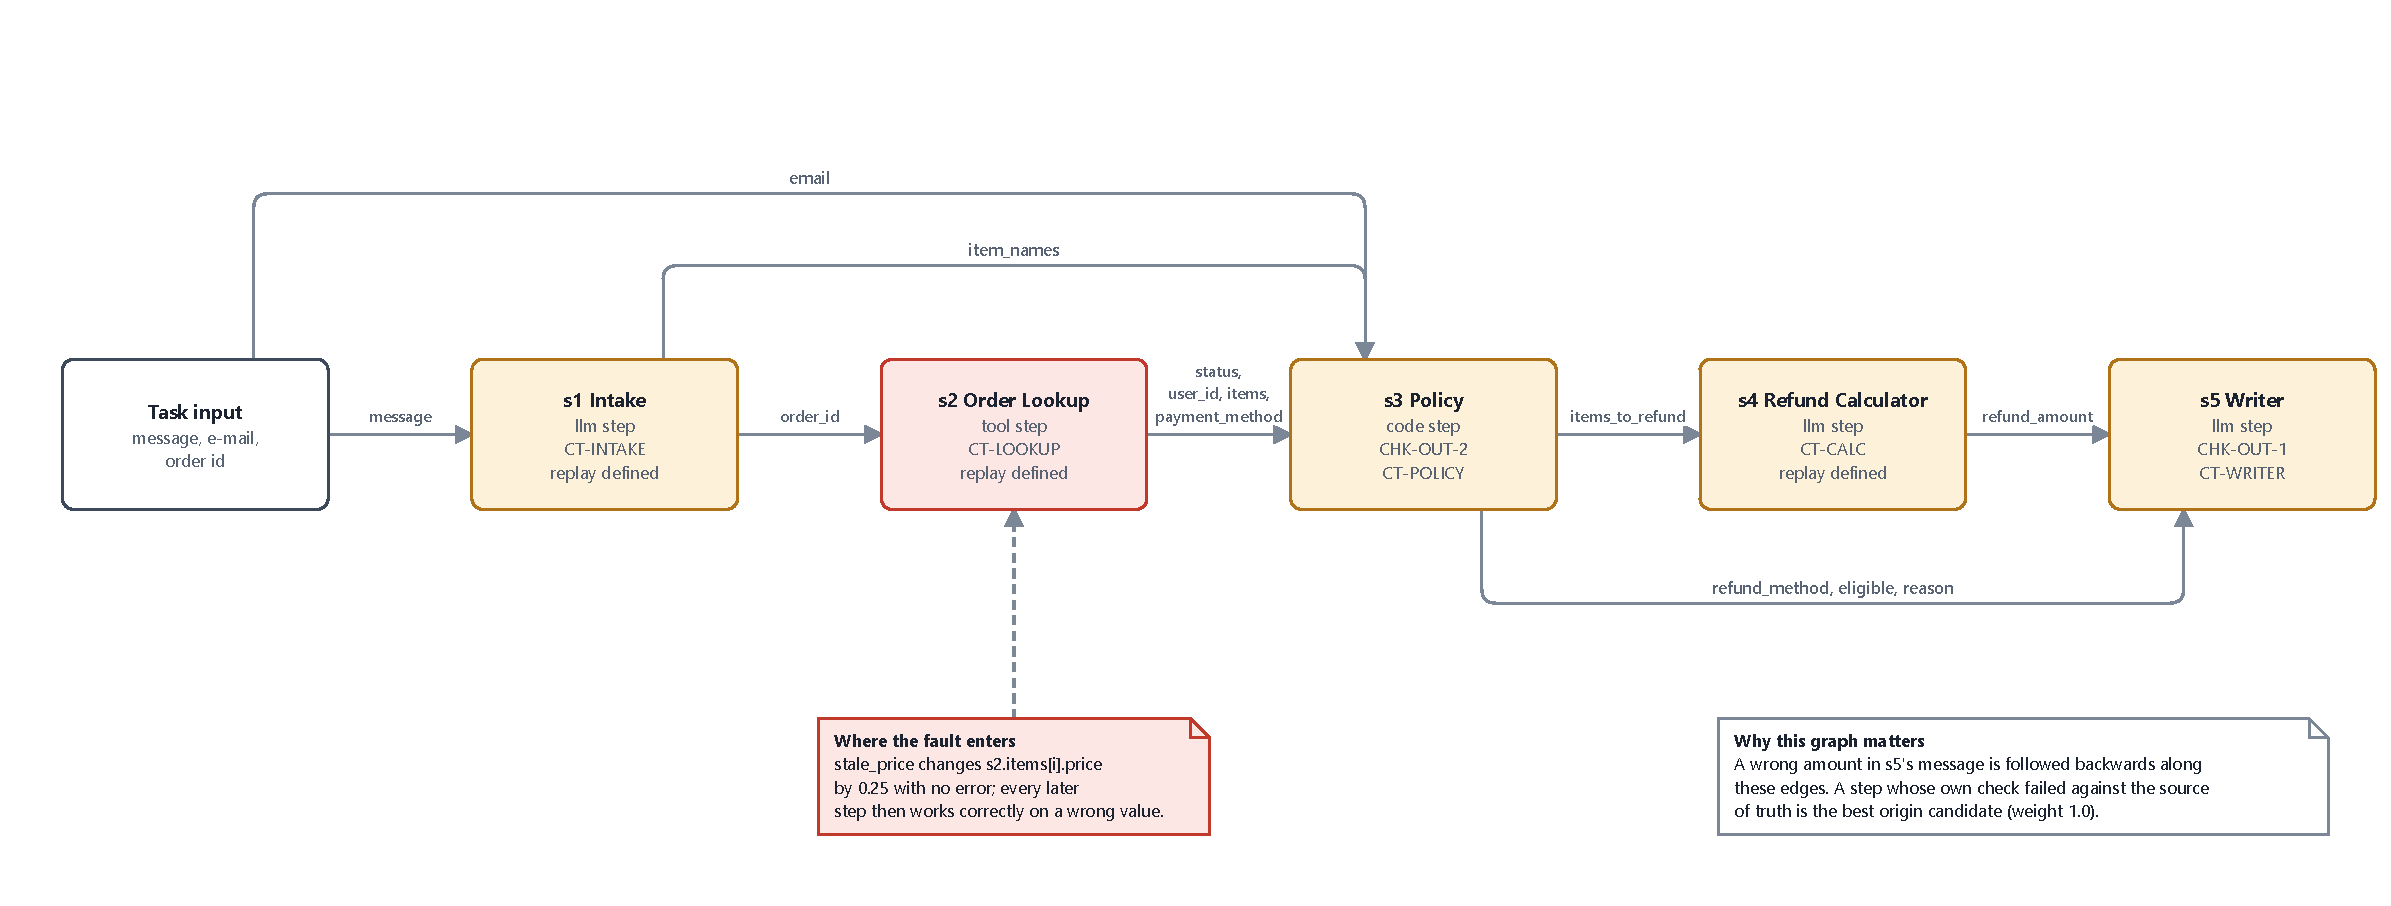
\includegraphics[width=\linewidth,height=0.62\textheight,keepaspectratio]{refund-desk-dataflow.pdf}
\caption{The Refund Desk workflow: five agents, the data each step reads, and the seven checks}
\label{fig:refund-dataflow}
\end{figure}


\section{Project Vision}

When a multi-agent AI workflow produces a wrong result, even one that raises no error, Granite tells the team where it went wrong, proves it, and shows whether a fix actually works, on infrastructure the team controls.

For developers and QA reviewers of multi-agent LLM workflows who need to know why a run produced a wrong result and whether a fix is real, Granite is a self-hostable investigation workbench that turns each suspected failure into a verified finding. Unlike debuggers whose diagnosis is mainly a language model's opinion over logs, Granite's findings rest on executable checks and controlled re-execution with controls, and it runs at zero cost on local or free models. Five principles guide the design: evidence before opinion; every finding is a record; say "inconclusive" when it is; a human decides; and every core path works offline.

\section{Project Objectives}

\begin{enumerate}
\item Detect silent failures in multi-agent runs using executable checks against an independent source of truth, with no false alarms on clean runs.
\item Localise the step where a failure began using deterministic data-flow provenance, and rank it first for faults that leave step-level evidence.
\item Verify a root-cause hypothesis by controlled replay, comparing N intervention replays against M control replays under a fixed, versioned verdict rule, and report INCONCLUSIVE honestly.
\item Record every finding as tamper-evident evidence with a human review and an exportable report.
\item Deliver this as a working, deployed product with a task-oriented interface, automated tests and CI/CD, running at zero cost.
\item Evaluate the system on a labelled benchmark with clean controls against baseline methods (from FYP-1 Final onward).
\end{enumerate}

\section{Project Scope}

\textbf{In scope:} running registered multi-agent workflows with optional fault injection; importing traces (Iteration 2); executable checks and silent-failure findings; provenance-based trace-back; replay verification with controls; human review and resolution; evidence, reports and history; a Fault Lab and evaluation module; a Python SDK with LangGraph and CrewAI adapters; self-hosting with local or recorded models.

\textbf{Out of scope for the whole FYP:} a multi-tenant SaaS with billing; Kubernetes or message queues; applying fixes automatically to a user's production system; training custom models; benchmarking on seven frameworks; a preventive classifier; and real customer data on the public demo.

\textbf{Scope table}

{\footnotesize\setlength{\tabcolsep}{3pt}
\begin{longtable}{>{\raggedright\arraybackslash\hspace{0pt}}p{0.094\linewidth}>{\raggedright\arraybackslash\hspace{0pt}}p{0.056\linewidth}>{\raggedright\arraybackslash\hspace{0pt}}p{0.196\linewidth}>{\raggedright\arraybackslash\hspace{0pt}}p{0.088\linewidth}>{\raggedright\arraybackslash\hspace{0pt}}p{0.159\linewidth}>{\raggedright\arraybackslash\hspace{0pt}}p{0.292\linewidth}}
\caption{Project Scope}\label{tab:chapter1_introduction-1}\\
\toprule
\textbf{Module} & \textbf{In / out at Mid-1} & \textbf{Proposal origin} & \textbf{Mid-1 status} & \textbf{Final-1 target} & \textbf{Success metric} \\
\midrule
\endfirsthead
\toprule
\textbf{Module} & \textbf{In / out at Mid-1} & \textbf{Proposal origin} & \textbf{Mid-1 status} & \textbf{Final-1 target} & \textbf{Success metric} \\
\midrule
\endhead
\bottomrule
\endlastfoot
M1 Run & In & Fault-injection harness & Done (Refund Desk) & + second workflow, 3 fault types & Runs recorded completely; reproducible in recorded mode \\
M2 Import & Out & SDK and adapters & Not started & Trace import, SDK + LangGraph & Imported runs validated with error paths \\
M3 Check & In & Semantic Error Diagnostic & Done & + check editor & Detection $\geq$ 90\%, false alarms 0 on clean runs \\
M4 Trace back & In & Culprit Agent, Error Step Localisation & Done & + cycle bound & Origin ranked first $\geq$ 80\% ($\geq$ 95\% over 20 runs as acceptance) \\
M5 Verify & In & Verification Agent, Verified Automatic Repair & Done & + resume & Verdict precision $\geq$ 85\% (evaluation) \\
M6 Review \& Resolve & In (review) & Repair Agent, Recovery Controller, Repair Memory & Review done & Fix suggestion, recovered run & Every decision recorded with reviewer and time \\
M7 Report & In (basic) & Dashboard & MD/JSON done & PDF, regression export & Every finding carries $\geq$ 1 reproducible evidence item \\
M8 Fault Lab \& Evaluation & Out & Cross-architecture benchmark & Feasibility run only & Benchmark v0 $\geq$ 120 runs, baselines & Metrics with confidence intervals \\
\end{longtable}
}

\section{Project Modules}

The ten mechanisms approved at the proposal were mapped one-to-one onto eight user-facing modules, so the approved idea is preserved while becoming understandable to users. \textbf{Run} executes a workflow on user input, optionally with an injected fault, and records a full trace. \textbf{Import} brings in traces from other tools through file upload, an SDK and framework adapters. \textbf{Check} evaluates executable checks on every run and turns silent failures into findings. \textbf{Trace back} ranks origin hypotheses by provenance, with an optional language-model second opinion labelled unverified. \textbf{Verify} tests a hypothesis or a proposed fix by controlled replay. \textbf{Review \& Resolve} records the human decision and, later, fix suggestions, recovered runs and a known-fix library. \textbf{Report} exports findings, regression tests and history. \textbf{Fault Lab \& Evaluation} generates labelled runs with clean controls and measures the system against baselines.

\section{Stakeholders and User Classes}

{\small
\begin{longtable}{>{\raggedright\arraybackslash\hspace{0pt}}p{0.159\linewidth}>{\raggedright\arraybackslash\hspace{0pt}}p{0.266\linewidth}>{\raggedright\arraybackslash\hspace{0pt}}p{0.222\linewidth}>{\raggedright\arraybackslash\hspace{0pt}}p{0.213\linewidth}}
\caption{Stakeholders and User Classes}\label{tab:chapter1_introduction-2}\\
\toprule
\textbf{User class} & \textbf{Context} & \textbf{Goal with Granite} & \textbf{Key need} \\
\midrule
\endfirsthead
\toprule
\textbf{User class} & \textbf{Context} & \textbf{Goal with Granite} & \textbf{Key need} \\
\midrule
\endhead
\bottomrule
\endlastfoot
Agent developer (primary) & Builds agent workflows at a software house, often for clients whose data cannot go to external services; small budget & Find why a run went wrong and prove a fix before shipping & Fast localisation, trustworthy verification, self-hosting \\
QA / reliability reviewer (primary) & Reviews incidents and signs off fixes & Decide accept or reject on clear evidence & Plain-language evidence, verdicts, an audit trail \\
Student / researcher & Builds multi-agent projects without paid tools & Learn why agents fail; test robustness & Free, local, explains failure modes \\
Auditor / client representative (secondary) & Receives incident reports & Proof of what failed and what was done & Exportable, tamper-evident reports \\
\end{longtable}
}

Other stakeholders are the end customers of the agent system (who need correct outcomes), privacy and compliance roles (redaction, retention, self-hosting), the supervisor and panel (academic standard and evaluation), the team (defensible individual ownership), and external parties such as model providers and framework maintainers (licences, rate limits). Four to six practitioner interviews are planned from Week 9 to validate these needs.

\section{Success Criteria}

{\small
\begin{longtable}{>{\raggedright\arraybackslash\hspace{0pt}}p{0.157\linewidth}>{\raggedright\arraybackslash\hspace{0pt}}p{0.534\linewidth}>{\raggedright\arraybackslash\hspace{0pt}}p{0.199\linewidth}}
\caption{Success Criteria}\label{tab:chapter1_introduction-3}\\
\toprule
\textbf{Area} & \textbf{Criterion} & \textbf{Mid-1 result} \\
\midrule
\endfirsthead
\toprule
\textbf{Area} & \textbf{Criterion} & \textbf{Mid-1 result} \\
\midrule
\endhead
\bottomrule
\endlastfoot
Detection & Injected faults detected in $\geq$ 90\% of faulty runs; 0 false alarms on clean runs & 10/10 detected; 0 false alarms \\
Attribution & True origin ranked first in $\geq$ 80\% of runs & 10/10 \\
Verification & True origin CONFIRMED in $\geq$ 80\%; innocent step REFUTED in $\geq$ 80\% & 9/10 and 10/10 \\
Reliability & $\geq$ 95\% of runs complete & 20/20 \\
Engineering & All automated tests pass; static analysis clean; CI green & 381/381; clean; green \\
Product & Core journey works live with failure cases; deployed URL & Done; live on Render \\
Usability (Final-1) & Task success $\geq$ 80\% unaided; SUS $\geq$ 68 & Protocol ready; sessions pending \\
Evaluation (Final-1/Mid-2) & Measured against last-agent and LLM-judge baselines with confidence intervals & Planned \\
\end{longtable}
}

\section{Constraints and Assumptions}

\textbf{Constraints:} zero recurring cost, so only local models, recorded answers and free hosting tiers are used; small local models (llama3.2:3b on a CPU) that are slow and make mistakes; free hosting that sleeps when idle and resets its disk; a three-person team with other courses; and a fixed academic calendar.

\textbf{Assumptions:} that a workflow can declare which earlier outputs each step reads, so data flow can be recorded rather than guessed; that a source of truth exists for the values being checked (here, the order and catalogue data); that replays can be made reproducible by pinning seeds and recording model answers; and that checks written by the operator capture what "correct" means. Granite can detect only failures that some check covers; this is a stated limit, not part of the definition of a failure.

\section{Ethical, Legal and DEI Considerations}

\textbf{Ethical.} Granite's output is advisory: a human reviews every finding, and the system never applies a fix to a production system on its own. Faults are injected only into the project's own workflows or, later, into those of consenting test participants. Trace data from a real system would be handled with redaction, retention limits and self-hosting, and any real user's data would require informed consent before use; the public demo uses synthetic data only.

\textbf{Legal.} Dataset and component licences are recorded: tau-bench retail data and Who\&When are MIT-licensed, the Llama 3.2 model is used under Meta's community licence with only its recorded answers distributed, and every software dependency is permissive. Granite's own licence is still to be chosen.

\textbf{DEI.} Automated failure diagnosis is today mostly sold as paid cloud services. Granite runs at zero cost on local models, so students, small teams and researchers in lower-resource settings get the same capability as well-funded teams. The interface does not convey status by colour alone, and automated accessibility checks run on every screen. We also state a coverage limit: the workflows and data are English-only, so results do not extend to non-English traces. The project aligns with SDG 9.5 (strengthening technological capability), as context rather than as a contribution claim.

%======================================================================================
% chapter2_research
%======================================================================================
\chapter{Research and Existing Solutions}

This chapter reviews the research and products related to failure diagnosis in multi-agent systems, compares them on the criteria that matter for silent failures, identifies the gap Granite addresses, and explains how the findings shaped the design. It also sets out why the problem is a complex computing problem.

\section{Research Method / Approach}

We studied the problem from four directions. First, we read seven research papers on multi-agent failure attribution in full, not only their abstracts: Who\&When (ICML 2025), AgenTracer (ICLR 2026), Scope Delineation Before Localization (SDBL, AAAI 2026), TraceElephant (ACL 2026), ErrorProbe (ACL 2026 Findings), AgentAsk (ACL 2026) and PROTEA (ACL 2026 Demonstrations), and added DoVer (ICLR 2026) after the proposal. For each we recorded the dataset, the ground truth, the reported accuracy and the authors' own stated limitations. Second, we compared commercial and open-source products from their public documentation. Third, we checked the department's entire published FYP archive, 660 registered titles from Spring 2019 to Fall 2025, for overlapping projects. Fourth, we ran eight proof-of-concept spikes to test the riskiest assumptions before committing to a design.

\section{Existing Solutions / Products}

\textbf{Research systems.} Who\&When~\cite{whowhen} formalised automated failure attribution and released a human-annotated benchmark; its best method reached only about 14\% step-level accuracy. AgenTracer~\cite{agentracer} generated training data by programmatic fault injection and counterfactual replay and trained an 8B model, reaching roughly 37--43\% step accuracy. SDBL~\cite{sdbl} first delineates the scope of a failure and then localises it, reaching 33--40\%. TraceElephant~\cite{traceelephant} showed that much of the difficulty came from incomplete traces and released full input-output traces. ErrorProbe~\cite{errorprobe} combines a failure taxonomy, symptom-driven backward tracing and a verification team of LLM agents with a verified memory, reaching about 59.5\% step accuracy. AgentAsk~\cite{agentask} intervenes at message hand-offs to prevent errors rather than diagnose them. PROTEA~\cite{protea} is an interactive tool that suggests prompt fixes and re-runs workflows after a developer adopts them. DoVer~\cite{dover}, the closest work to ours, validates failure hypotheses by intervening at the suspected step and re-executing, flipping 18--28\% of failed trials on GAIA and AssistantBench.

\textbf{Products.} LangSmith Engine~\cite{langsmith} clusters production failures, diagnoses root causes against code and drafts fixes, but only inside LangSmith. Patronus Percival~\cite{percival} detects over twenty failure modes in traces with LLM judges and suggests prompt fixes. Galileo's Insights Engine~\cite{galileo} identifies failure modes and links them to spans. Raindrop~\cite{raindrop} markets silent-failure detection in production agents based on conversation signals and offers experiments to validate fixes. Invariant Labs' analyzer~\cite{invariant} runs rule-based checks over agent traces with a security focus. Langfuse, Arize Phoenix, Braintrust, Weights \& Biases Weave and Opik capture traces and run evaluations, leaving diagnosis to people.

\textbf{Prior FYPs.} None of the 660 titles in the department archive targets the same problem. Multi-agent systems appear only as the product itself (an agent team that does a task), never as the object being diagnosed. The closest neighbour is a Spring 2024 project on hallucination detection in a single model's text output, which has no multi-agent attribution or verification.

\section{Comparison of Existing Solutions}

\begin{landscape}
{\footnotesize\setlength{\tabcolsep}{3pt}
\begin{longtable}{>{\raggedright\arraybackslash\hspace{0pt}}p{0.088\linewidth}>{\raggedright\arraybackslash\hspace{0pt}}p{0.082\linewidth}>{\raggedright\arraybackslash\hspace{0pt}}p{0.125\linewidth}>{\raggedright\arraybackslash\hspace{0pt}}p{0.121\linewidth}>{\raggedright\arraybackslash\hspace{0pt}}p{0.139\linewidth}>{\raggedright\arraybackslash\hspace{0pt}}p{0.099\linewidth}>{\raggedright\arraybackslash\hspace{0pt}}p{0.086\linewidth}>{\raggedright\arraybackslash\hspace{0pt}}p{0.102\linewidth}}
\caption{Comparison of Existing Solutions}\label{tab:chapter2_research-1}\\
\toprule
\textbf{Solution} & \textbf{Type} & \textbf{Detects silent failures?} & \textbf{Localises origin step?} & \textbf{Verifies cause by re-execution?} & \textbf{Handles model non-determinism?} & \textbf{Self-hosted, \$0?} & \textbf{Accuracy published?} \\
\midrule
\endfirsthead
\toprule
\textbf{Solution} & \textbf{Type} & \textbf{Detects silent failures?} & \textbf{Localises origin step?} & \textbf{Verifies cause by re-execution?} & \textbf{Handles model non-determinism?} & \textbf{Self-hosted, \$0?} & \textbf{Accuracy published?} \\
\midrule
\endhead
\bottomrule
\endlastfoot
Who\&When & Research & No & Yes (LLM) & No & No & Research code & Yes (\textasciitilde{}14\% step) \\
AgenTracer & Research & No & Yes (trained model) & Counterfactual for labelling & No & Partly released & Yes (\textasciitilde{}37--43\%) \\
ErrorProbe & Research & No (named as a limitation) & Yes (LLM team) & Tool-grounded checks & No & Research code & Yes (\textasciitilde{}59.5\%) \\
DoVer & Research & No & Uses given hypotheses & Yes (intervention) & Single re-execution & Research code & Flip rates (18--49\%) \\
PROTEA & Research demo & No & Node level & Re-runs after a human fix & No & Closed & Case studies only \\
LangSmith Engine & Commercial & Partly & Yes (LLM) & Reopens on regression & Not documented & No (SaaS) & No \\
Patronus Percival & Commercial & Failure modes via LLM judges & Yes (LLM) & Not documented & No & No (SaaS) & No \\
Raindrop & Commercial & Yes (conversation signals) & No step-level attribution & Experiments & Not documented & No (SaaS) & No \\
Invariant analyzer & Open source & Rule-based checks & No & No & n/a & Yes & n/a \\
\textbf{Granite} & \textbf{This project} & \textbf{Yes (executable checks + source of truth)} & \textbf{Yes (deterministic provenance)} & \textbf{Yes (N replays + M controls)} & \textbf{Yes (controls, verdict rule, INCONCLUSIVE)} & \textbf{Yes} & \textbf{Pre-registered; benchmark planned} \\
\end{longtable}
}
\end{landscape}

\section{Limitations and Gaps}

Three gaps recur. First, \textbf{silent failures}: attribution methods assume a failure leaves an anomaly; ErrorProbe's own limitations section names silent failures, outputs that are valid but semantically wrong, as a case it cannot handle, and points to "test-time oracle feedback" as future work. Second, \textbf{verification under non-determinism}: where hypotheses are re-tested by re-execution (DoVer, PROTEA, commercial "experiments"), a single re-run is used, so a fix can appear to work by chance and the result is not compared against controls. Third, \textbf{trust and access}: commercial diagnoses are language-model opinions, delivered as cloud services that some teams cannot use with client data, with no published accuracy. Benchmarks in the field also contain only failures, with no clean controls, so false-alarm rates are not measured.

\section{Proposed Solution}

Granite addresses these gaps with a self-hostable product that: (1) detects silent failures with operator-declared executable checks against an independent source of truth, the test-time oracles ErrorProbe names as future work; (2) localises the origin with deterministic value-provenance tracing over the run's data flow, with no language model in the core path; and (3) verifies each hypothesis with a controlled replay protocol, N intervention replays and M control replays under a pre-registered, versioned verdict rule, recording every artefact as hashed evidence for a human reviewer. We will evaluate it on a labelled fault-injection benchmark with clean controls against last-agent and LLM-judge baselines, measuring origin accuracy, false-alarm rate, verdict precision and recovery rate.

We no longer claim to be "first" or that "nobody verifies fixes": DoVer and several products already re-execute or experiment. Our contribution is the combination of executable-check detection, deterministic attribution and a verification protocol with controls, measured honestly and runnable at zero cost.

\section{Complex Computing Problem}

{\small
\begin{longtable}{>{\raggedright\arraybackslash\hspace{0pt}}p{0.312\linewidth}>{\raggedright\arraybackslash\hspace{0pt}}p{0.608\linewidth}}
\caption{Complex Computing Problem}\label{tab:chapter2_research-2}\\
\toprule
\textbf{Seoul Accord characteristic~\cite{seoulaccord}} & \textbf{How Granite meets it} \\
\midrule
\endfirsthead
\toprule
\textbf{Seoul Accord characteristic~\cite{seoulaccord}} & \textbf{How Granite meets it} \\
\midrule
\endhead
\bottomrule
\endlastfoot
1. Conflicting requirements & Verification confidence versus replay cost and latency; privacy (local model) versus model quality; detection sensitivity versus false alarms \\
2. No obvious solution & Published attribution reaches about 60\% step accuracy at best; single-replay verification is unreliable under non-determinism \\
3. Depth of knowledge & Graph and provenance algorithms, statistics (interval estimates, controls), LLM behaviour, sandboxed evaluation \\
4. Unfamiliar issues & Non-deterministic re-execution; failures that appear several steps after their cause \\
5. Beyond standard practice & Not solvable with a tracing library or a CRUD application \\
6. Diverse stakeholders & Developers, reviewers, end customers, auditors, privacy roles (to be strengthened with interviews) \\
7. Significant consequences & Wrong refunds, wrong advice, money moved on wrong numbers \\
8. Interdependence & Failures propagate through dependent agents and steps \\
9. Ill-defined cause & Whether a failure exists, where it began and what the correct value is are all unknown at diagnosis time \\
\end{longtable}
}

\section{Technical Challenges}

The main challenges are: making replays reproducible enough that a verdict means something when the model is non-deterministic (solved with recorded answers, pinned seeds and control replays); evaluating user-written check expressions safely without allowing code execution (solved with our own evaluator over a whitelist of syntax nodes); attributing a failure without leaking the injected fault's ground truth into the analysis (enforced by a test); keeping upstream outputs fixed while re-running only the downstream steps; handling small local models that are slow (5--35 seconds per call on a CPU) and make arithmetic errors; and keeping design documents consistent with fast-changing code (solved by generating diagrams from the code and checking them in CI).

\section{Research Findings and Design Decisions}

{\small
\begin{longtable}{>{\raggedright\arraybackslash\hspace{0pt}}p{0.460\linewidth}>{\raggedright\arraybackslash\hspace{0pt}}p{0.460\linewidth}}
\caption{Research Findings and Design Decisions}\label{tab:chapter2_research-3}\\
\toprule
\textbf{Finding (source)} & \textbf{Design decision} \\
\midrule
\endfirsthead
\toprule
\textbf{Finding (source)} & \textbf{Design decision} \\
\midrule
\endhead
\bottomrule
\endlastfoot
LLM-based attribution reaches only 14--60\% step accuracy (Who\&When, AgenTracer, SDBL, ErrorProbe); our own reproduction with a 3B model reached 0--25\% step accuracy over five runs (Spike 1) & Core attribution is deterministic provenance; an LLM opinion is optional and labelled unverified (ADR-005) \\
ErrorProbe names silent failures and test-time oracles as open & Detection uses executable checks against a source of truth, not an answer key (ADR-004) \\
A single re-run can pass by chance; our replay spike worked but n was tiny (Spike 5) & Verification uses N = 5 intervention replays plus M = 2 controls under a fixed rule VR-1 (ADR-006) \\
Run-to-run variance of small models is large (Spike 1 rerun five times) & Results are reported as ranges and intervals, thresholds are pre-registered \\
TraceElephant: incomplete traces limit diagnosis & Every step records its full inputs, outputs and declared reads (Granite Trace v1, ADR-009) \\
Fault injection gives exact ground truth (AgenTracer; Spike 3b) & Faults are rule-based and their ground truth is stored but hidden from attribution \\
A preventive classifier gave near-random signal (Spike 7) & Dropped from scope and reported as a negative result \\
DoVer and commercial tools already re-execute or diagnose & Novelty re-baselined to checks + provenance + controls + self-hosting \\
Cost estimate from measured token counts & Zero-cost design: local Ollama model and recorded answers (ADR-008) \\
\end{longtable}
}

%======================================================================================
% chapter3_iteration_plan
%======================================================================================
\chapter{Proposal Feedback and Iteration Plan}

This chapter summarises the feedback received at the proposal defense, records how each comment was addressed, and describes the iterative plan: what Iteration 1 delivered, what Iteration 2 will add, who is responsible for what, and how progress compares with the plan, including delays and the recovery actions taken.

\section{Proposal Feedback Summary}

The proposal was approved at the defense on 11 September 2026 with five comments from the panel: (1) "UI/UX needs improvement"; (2) "Features are not sufficiently clear"; (3) "It is unclear what inputs each feature will accept"; (4) "It is unclear how identified flaws/issues will be verified and how verification results will be captured"; and (5) "The overall project workflow must be redefined." We also recorded an implicit sixth point: the proof of concept demonstrated research results rather than a product.

Analysing the comments together, we concluded that they shared one root cause: we had designed mechanisms, not a user workflow. The proof-of-concept console only displayed pre-recorded spike results; there was no screen where a user could give Granite something and get back a verified result. Our response was to redefine the product around one workflow and one unit of value, the verified finding.

\section{Proposal Action Register}

{\small
\begin{longtable}{>{\raggedright\arraybackslash\hspace{0pt}}p{0.025\linewidth}>{\raggedright\arraybackslash\hspace{0pt}}p{0.179\linewidth}>{\raggedright\arraybackslash\hspace{0pt}}p{0.266\linewidth}>{\raggedright\arraybackslash\hspace{0pt}}p{0.119\linewidth}>{\raggedright\arraybackslash\hspace{0pt}}p{0.241\linewidth}}
\caption{Proposal Action Register}\label{tab:chapter3_iteration_plan-1}\\
\toprule
\textbf{No.} & \textbf{Feedback / Required change} & \textbf{Action taken} & \textbf{Status} & \textbf{Evidence} \\
\midrule
\endfirsthead
\toprule
\textbf{No.} & \textbf{Feedback / Required change} & \textbf{Action taken} & \textbf{Status} & \textbf{Evidence} \\
\midrule
\endhead
\bottomrule
\endlastfoot
A1 & UI/UX needs improvement & Replaced the PoC console with five task-oriented screens (investigations, new run, run, finding, guide), a four-stage stepper, loading/empty/error states, light and dark themes, phone layout, keyboard-operable graph; automated accessibility checks; before/after comparison & Partly done (usability test with outside users pending) & Screenshots and before/after record in \texttt{evidence/\allowbreak{}demos/\allowbreak{}}; accessibility audit \\
A2 & Features not sufficiently clear & Collapsed ten mechanism names into eight plainly named features in one fixed order; the same list is a page in the product & Done & Feature catalogue; in-app "How it works" page \\
A3 & Unclear what inputs each feature accepts & Every input has a type, a limit and a refusal message, enforced by the server and covered by tests; published trace schema; API documentation & Done & Data dictionary; validation tests; \texttt{/\allowbreak{}docs} \\
A4 & Unclear how flaws are verified and results captured & Verification levels V0--V3; replay with N fixes and M controls under rule VR-1 with a Wilson interval; hashed append-only evidence; review records; exportable report & Done & Verification sequence diagram; decision-table tests; feasibility results \\
A5 & Overall workflow must be redefined & One workflow (run, check, detect, trace back, verify, review, resolve, record), enforced by a state machine and shown as a stepper & Done (change record C-01 awaits signature) & State machine; flow and activity diagrams \\
A6 & PoC showed research, not a product & Working vertical slice with CI/CD, deployed publicly & Partly done (CD hook and tag pending) & Live URL; CI and CD runs; deployment record \\
\end{longtable}
}

Figure~\ref{fig:ui-before-after} compares the screens shown at the defense with the product at Mid-1.

\begin{figure}[htbp]
\centering
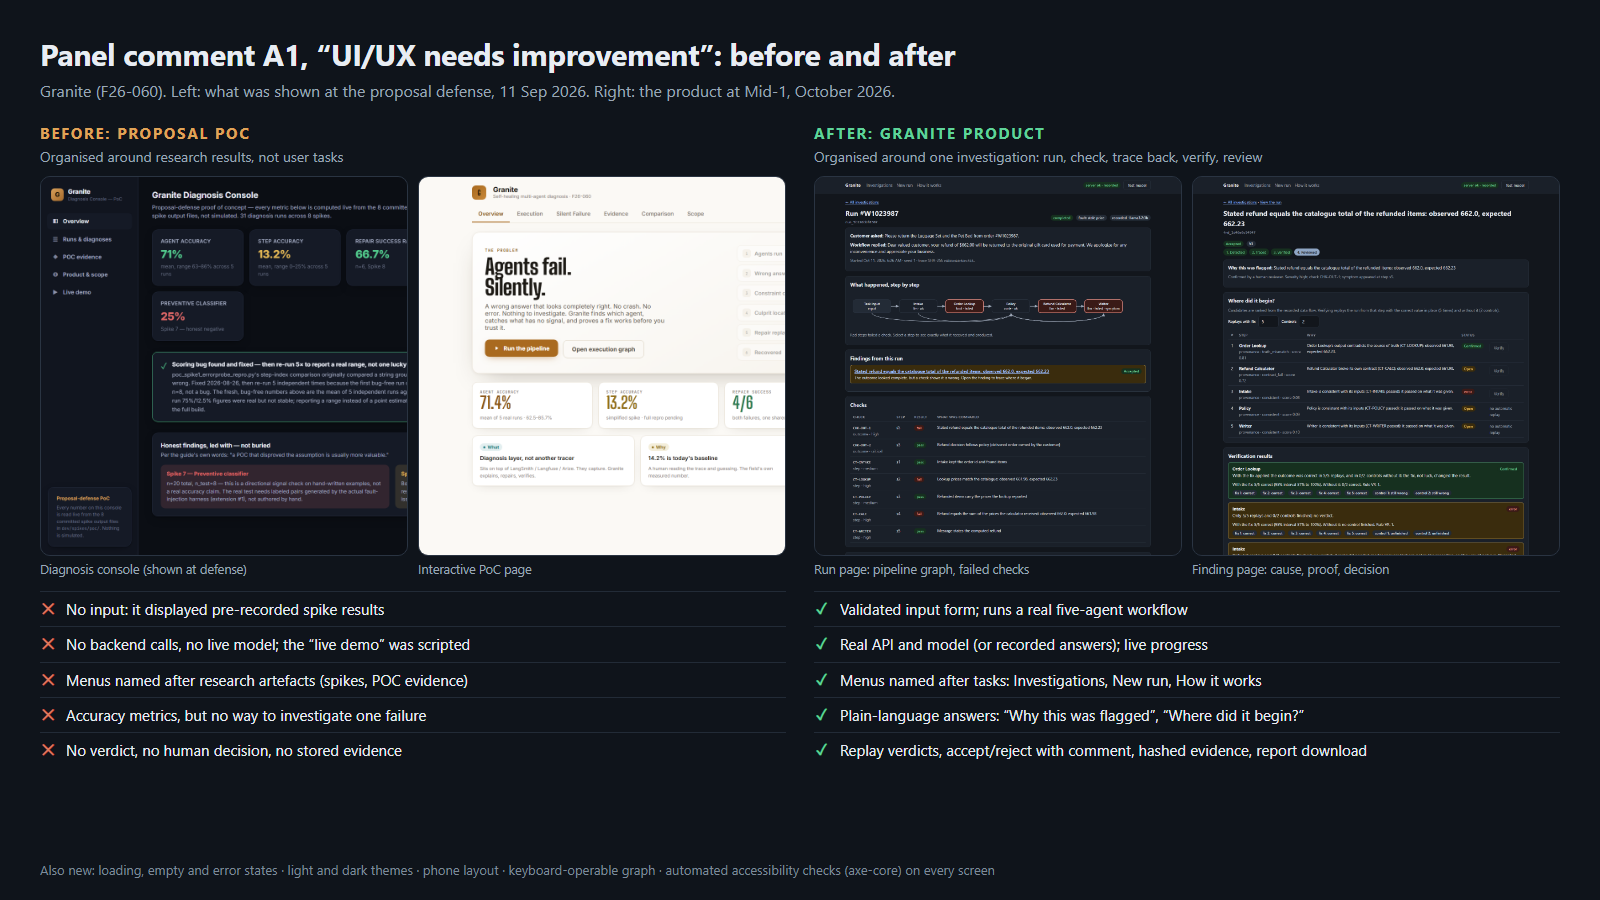
\includegraphics[width=\linewidth,height=0.42\textheight,keepaspectratio]{2026-10-13_ui-before-after.png}
\caption{Panel comment A1: the proposal-defense PoC (left) compared with the Mid-1 product (right)}
\label{fig:ui-before-after}
\end{figure}


\section{Iteration Strategy}

We follow an iterative, incremental strategy in which every iteration ends with a working, demonstrable product rather than documents. Iteration 1 builds one complete vertical slice, a single workflow and fault taken through every stage from run to report, so that the whole investigation loop is proven before breadth is added. Later iterations add inputs (import, SDK), more workflows and faults, repair and recovery, and the evaluation. Each iteration has a release tag, scope is prioritised with MoSCoW per milestone, and changes to scope or design are recorded in a change log before results are known.

\section{Iteration 1 Plan}

\textbf{Objective:} a working core investigation slice for Mid-1 (release v0.1.0). \textbf{Use cases:} UC-03 run a workflow, UC-05 inspect a run, UC-06 analyse a run, UC-07 investigate a finding, UC-08 verify a hypothesis, UC-09 review a finding, UC-12 browse history (and UC-11 export report as a Should). \textbf{Deliverables:} the core library (trace, runner, check language, checks, attribution, verification, lifecycle, evidence), the Refund Desk workflow on real data with a real local model, the API with database and background jobs, the web interface, CI/CD, a pre-registered feasibility run, the design artefacts of handbook Table 1a, system tests and manuals. \textbf{Evidence:} live demonstration, automated test results, CI runs, generated diagrams and the feasibility results.

\section{Iteration 2 Plan}

\textbf{Objective:} breadth and inputs, reaching FYP-1 Final (release v0.2.0) with about half of the committed effort implemented. \textbf{Use cases:} UC-01 configure project, UC-02 define and test checks, UC-04 import a trace, UC-10 suggest and verify a fix, UC-11 export report and regression test, UC-13 Fault Lab, UC-14 evaluation v0, UC-15 SDK with LangGraph. \textbf{Deliverables:} trace import, a second workflow, three fault types, a check editor, PII redaction, fix suggestion and recovered runs, PDF reports, the SDK and LangGraph adapter, a benchmark of at least 120 runs with baselines, a usability pilot and an install by a non-owner.

\section{Work Breakdown and Responsibilities}

{\small
\begin{longtable}{>{\raggedright\arraybackslash\hspace{0pt}}p{0.093\linewidth}>{\raggedright\arraybackslash\hspace{0pt}}p{0.127\linewidth}>{\raggedright\arraybackslash\hspace{0pt}}p{0.320\linewidth}>{\raggedright\arraybackslash\hspace{0pt}}p{0.320\linewidth}}
\caption{Work Breakdown and Responsibilities}\label{tab:chapter3_iteration_plan-2}\\
\toprule
\textbf{Member} & \textbf{Area} & \textbf{Iteration 1 modules} & \textbf{Iteration 2 work} \\
\midrule
\endfirsthead
\toprule
\textbf{Member} & \textbf{Area} & \textbf{Iteration 1 modules} & \textbf{Iteration 2 work} \\
\midrule
\endhead
\bottomrule
\endlastfoot
Shahoud Shahid & Workflows, Data \& Experience & Runner, Refund Desk workflow, faults, LLM providers, web interface shell & Trace import, more fault types, redaction, SDK and LangGraph adapter, Fault Lab, help page \\
Muhammad Noor Ul Haq & Investigation Engine & Check language and checks, attribution, feasibility evaluation & Check editor, attribution cycle bound, fix D-25, second workflow's checks, evaluation harness and baselines, evaluation screen \\
Saif Shahzad & Verification \& Platform & Verification and verdict rule, lifecycle, API, database, jobs, CI/CD & Experiment resume, fix suggestion and recovered run, regression export, PDF reports, release pipeline, non-owner install \\
\end{longtable}
}

\section{Progress Against Plan}

Iteration 1 items 1 to 13 (planning, workspace, core library, attribution, verification, workflow, API, interface, feasibility run, CI, design artefacts, system tests and manuals, panel action register) were completed between 6 and 11 October, and the public deployment followed on 11 October. The items behind schedule are fully automated deployment (the CD workflow runs but its deploy step awaits a repository secret), branch protection and the release tag, pull requests from every member, the code walkthroughs, redaction before storage, and the usability check. All 381 automated tests pass and the feasibility run met every pre-registered threshold.

\section{Delays, Deviations and Recovery Plan}

\textbf{Delays.} No commits were made for three weeks after the defense, while the team redefined the workflow in response to the panel; the product was then built in a compressed, AI-assisted effort between 6 and 11 October, committed largely from one account. As a result, work is not yet visible under its planned owners and no member has yet demonstrated a file-level walkthrough.

\textbf{Recovery.} Each owner completes the code-walkthrough exercise for their module before the evaluation and contributes from now on only through reviewed pull requests from their own account; the first two pull requests were opened on 11 October. A repository admin adds the deploy-hook secret, protects \texttt{main} and tags v0.1.0-mid1 before the meeting. The usability check runs in Week 9 and redaction is built in Week 10.

\textbf{Deviations from the plan, recorded in the change log:} C-01 (workflow redefined around the verified finding; awaits the supervisor's signature); C-02 (implementation decisions such as a 120-second timeout for local models, one finding per failing outcome check, the policy step implemented as deterministic code, and redaction deferred); and C-03 (diagrams generated from code, simplified branching, an added system test level, a CD workflow, and enforced docstring and naming rules).

%======================================================================================
% chapter4_requirements
%======================================================================================
\chapter{Software Requirements}

Granite's requirements are organised by product module. Each functional requirement has an identifier, a priority (M Must, S Should), the milestone where it is due and a testable acceptance criterion. Requirements for Mid-1 are traced to the code that implements them and the tests that check them, and a script in CI fails if a traced file or test does not exist.

\section{User Interactions / Use Cases}

The system has two primary human actors and two external systems. The \textbf{Developer} runs and investigates workflows; the \textbf{Reviewer} decides whether a finding is accepted (in a small team, the same person may play both roles). An \textbf{Administrator} operates a self-hosted instance (FYP-2). The \textbf{LLM Provider} (a local Ollama model, a hosted endpoint or recorded answers) answers the workflow's language-model steps, and an \textbf{Instrumented Workflow} sends traces through the SDK (Iteration 2).

{\small
\begin{longtable}{>{\raggedright\arraybackslash\hspace{0pt}}p{0.099\linewidth}>{\raggedright\arraybackslash\hspace{0pt}}p{0.398\linewidth}>{\raggedright\arraybackslash\hspace{0pt}}p{0.197\linewidth}>{\raggedright\arraybackslash\hspace{0pt}}p{0.166\linewidth}}
\caption{User Interactions / Use Cases}\label{tab:chapter4_requirements-1}\\
\toprule
\textbf{UC} & \textbf{Name} & \textbf{Actor} & \textbf{Milestone} \\
\midrule
\endfirsthead
\toprule
\textbf{UC} & \textbf{Name} & \textbf{Actor} & \textbf{Milestone} \\
\midrule
\endhead
\bottomrule
\endlastfoot
UC-01 & Configure project (workflow, settings) & Developer & Mid-1 seeded; Final-1 editable \\
UC-02 & Define, edit and dry-run checks & Developer & Final-1 \\
\textbf{UC-03} & \textbf{Run workflow with input (optional fault)} & Developer & \textbf{Mid-1} \\
UC-04 & Import trace file & Developer & Final-1 \\
\textbf{UC-05} & \textbf{Inspect run trace (graph, steps, checks)} & Developer, Reviewer & \textbf{Mid-1} \\
\textbf{UC-06} & \textbf{Analyse run (checks $\rightarrow$ findings $\rightarrow$ hypotheses)} & System, included by UC-03/04 & \textbf{Mid-1} \\
\textbf{UC-07} & \textbf{Investigate finding} & Developer, Reviewer & \textbf{Mid-1} \\
\textbf{UC-08} & \textbf{Verify hypothesis by controlled replay} & Developer, LLM Provider & \textbf{Mid-1} \\
\textbf{UC-09} & \textbf{Review finding (accept / reject / request information)} & Reviewer & \textbf{Mid-1} \\
UC-10 & Suggest and verify a fix; produce a recovered run & Developer, LLM Provider & Final-1 \\
UC-11 & Export report / regression test & Developer, Reviewer & Mid-1 (report); Final-1 (regression) \\
\textbf{UC-12} & \textbf{Browse and search history} & Developer, Reviewer & \textbf{Mid-1} \\
UC-13 & Generate labelled benchmark (Fault Lab) & Developer & Final-1 \\
UC-14 & Run evaluation against baselines & Developer (research) & Final-1 v0 / Mid-2 \\
UC-15 & Instrument own workflow via SDK & Developer, Instrumented Workflow & Final-1 (LangGraph), Mid-2 (CrewAI) \\
UC-16 & Reuse a known verified fix & Developer & Mid-2 \\
UC-17 & Manage API keys, retention, delete data & Administrator & Mid-2 \\
\end{longtable}
}

\section{Use Case Diagram}

Figure~\ref{fig:use-case-diagram} shows the Developer and Reviewer interacting with the Mid-1 use cases. Running a workflow (UC-03) always includes analysing the run (UC-06), which evaluates the checks, opens findings and ranks hypotheses. Investigating a finding (UC-07) extends to verification (UC-08), which involves the LLM Provider, and review (UC-09). Planned use cases for Iteration 2 and FYP-2 are shown separately.

\begin{figure}[htbp]
\centering
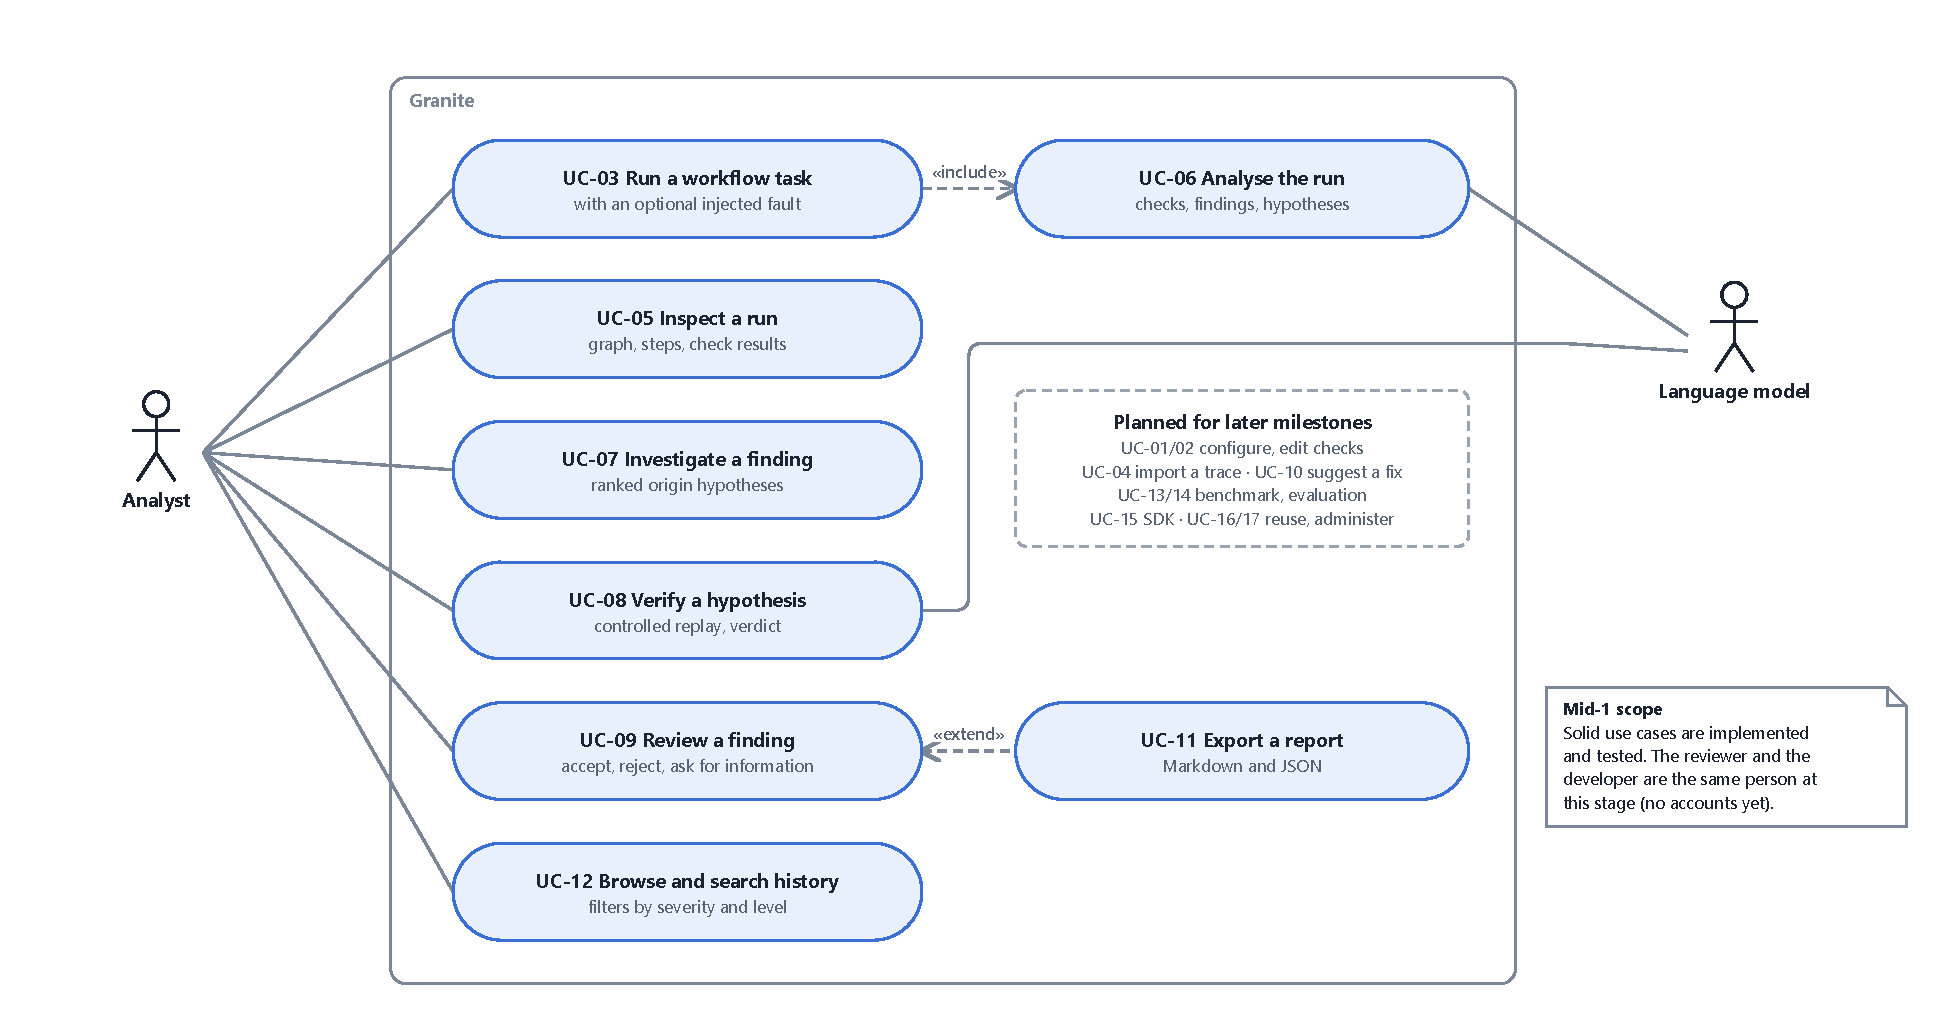
\includegraphics[width=\linewidth,height=0.42\textheight,keepaspectratio]{use-case-diagram.pdf}
\caption{Use case diagram (implemented and planned use cases are drawn differently)}
\label{fig:use-case-diagram}
\end{figure}


\section{Detailed Use Cases}

\textbf{UC-03 Run workflow with input}

\begin{itemize}
\item \textit{Actor:} Developer. \textit{Precondition:} the Refund Desk workflow is registered; the server is reachable.
\item \textit{Main flow:} (1) The developer opens New run and loads an example or types a request, e-mail and order number. (2) The developer optionally selects the fault "stale price" and the model mode. (3) The developer presses Run workflow. (4) The system validates the input, stores a queued run and returns a job. (5) The system executes the five steps, records each step's inputs, outputs and timing, and applies the fault if selected. (6) The system analyses the run (UC-06) and shows the run page with the pipeline graph, the check results and any findings.
\item \textit{Alternative flows:} 4a. A field is invalid: the system refuses the run and shows one plain message per field. 5a. The model is unreachable or a task has no recorded answers: the run ends as "errored" with the reason and a "Run again" button. 5b. Too many requests in a minute: the system answers "too many requests" (429).
\item \textit{Postcondition:} a completed or errored run is stored with its trace and SHA-256 hash.
\end{itemize}

\textbf{UC-07 Investigate finding}

\begin{itemize}
\item \textit{Actor:} Developer or Reviewer. \textit{Precondition:} a finding exists.
\item \textit{Main flow:} (1) The user opens the finding from the run page or the investigations list. (2) The system shows why it was flagged (the failed check with observed and expected values), the stage in the four-step stepper, and the ranked hypotheses under "Where did it begin?", each with its step, evidence type, score and a plain-language reason. (3) The user opens the evidence records to see the computation and its hash status.
\item \textit{Alternative flow:} 2a. No step has direct evidence: hypotheses are ranked structurally and labelled as needing verification.
\end{itemize}

\textbf{UC-08 Verify hypothesis by controlled replay}

\begin{itemize}
\item \textit{Actor:} Developer; LLM Provider. \textit{Precondition:} a hypothesis exists for a step with a repair rule.
\item \textit{Main flow:} (1) The user sets the number of replays with the fix (default 5) and controls (default 2) and presses Verify. (2) The system builds an intervention that replaces the step's output with the corrected value, keeps all earlier outputs fixed, and re-executes the later steps N times with the fix and M times without it. (3) The system applies rule VR-1 to the pass counts and shows the verdict (CONFIRMED, REFUTED or INCONCLUSIVE), the per-replay results and a 95\% Wilson interval, and stores the verdict as evidence. (4) The finding moves to the matching state.
\item \textit{Alternative flows:} 2a. The step has no repair rule: the system refuses the verification and says why. 2b. Replays need model answers that are not recorded: the experiment ends with no verdict and an explanation that a live model is required. 3a. REFUTED: the user verifies the next hypothesis.
\end{itemize}

\textbf{UC-09 Review finding}

\begin{itemize}
\item \textit{Actor:} Reviewer. \textit{Precondition:} the finding is CONFIRMED, INCONCLUSIVE or evidence-supported.
\item \textit{Main flow:} (1) The reviewer reads the evidence and verdict. (2) The reviewer chooses Accept, Reject or Ask for information, with a name and a comment. (3) The system checks the comment rule, moves the finding to its new state, records the review with reviewer and time, adds the comment as evidence and writes an audit entry. (4) After acceptance, the reviewer can mark the finding resolved or close it without fixing.
\item \textit{Alternative flows:} 2a. Reject, close or accepting an inconclusive finding without a comment of at least five characters: refused (422). 2b. An action not allowed in the current state (for example accepting before verification): refused (409) with the allowed actions.
\end{itemize}

Figures~\ref{fig:run-sequence} and~\ref{fig:verification-sequence-uc} show the system sequences for running a workflow and verifying a hypothesis.

\begin{figure}[htbp]
\centering
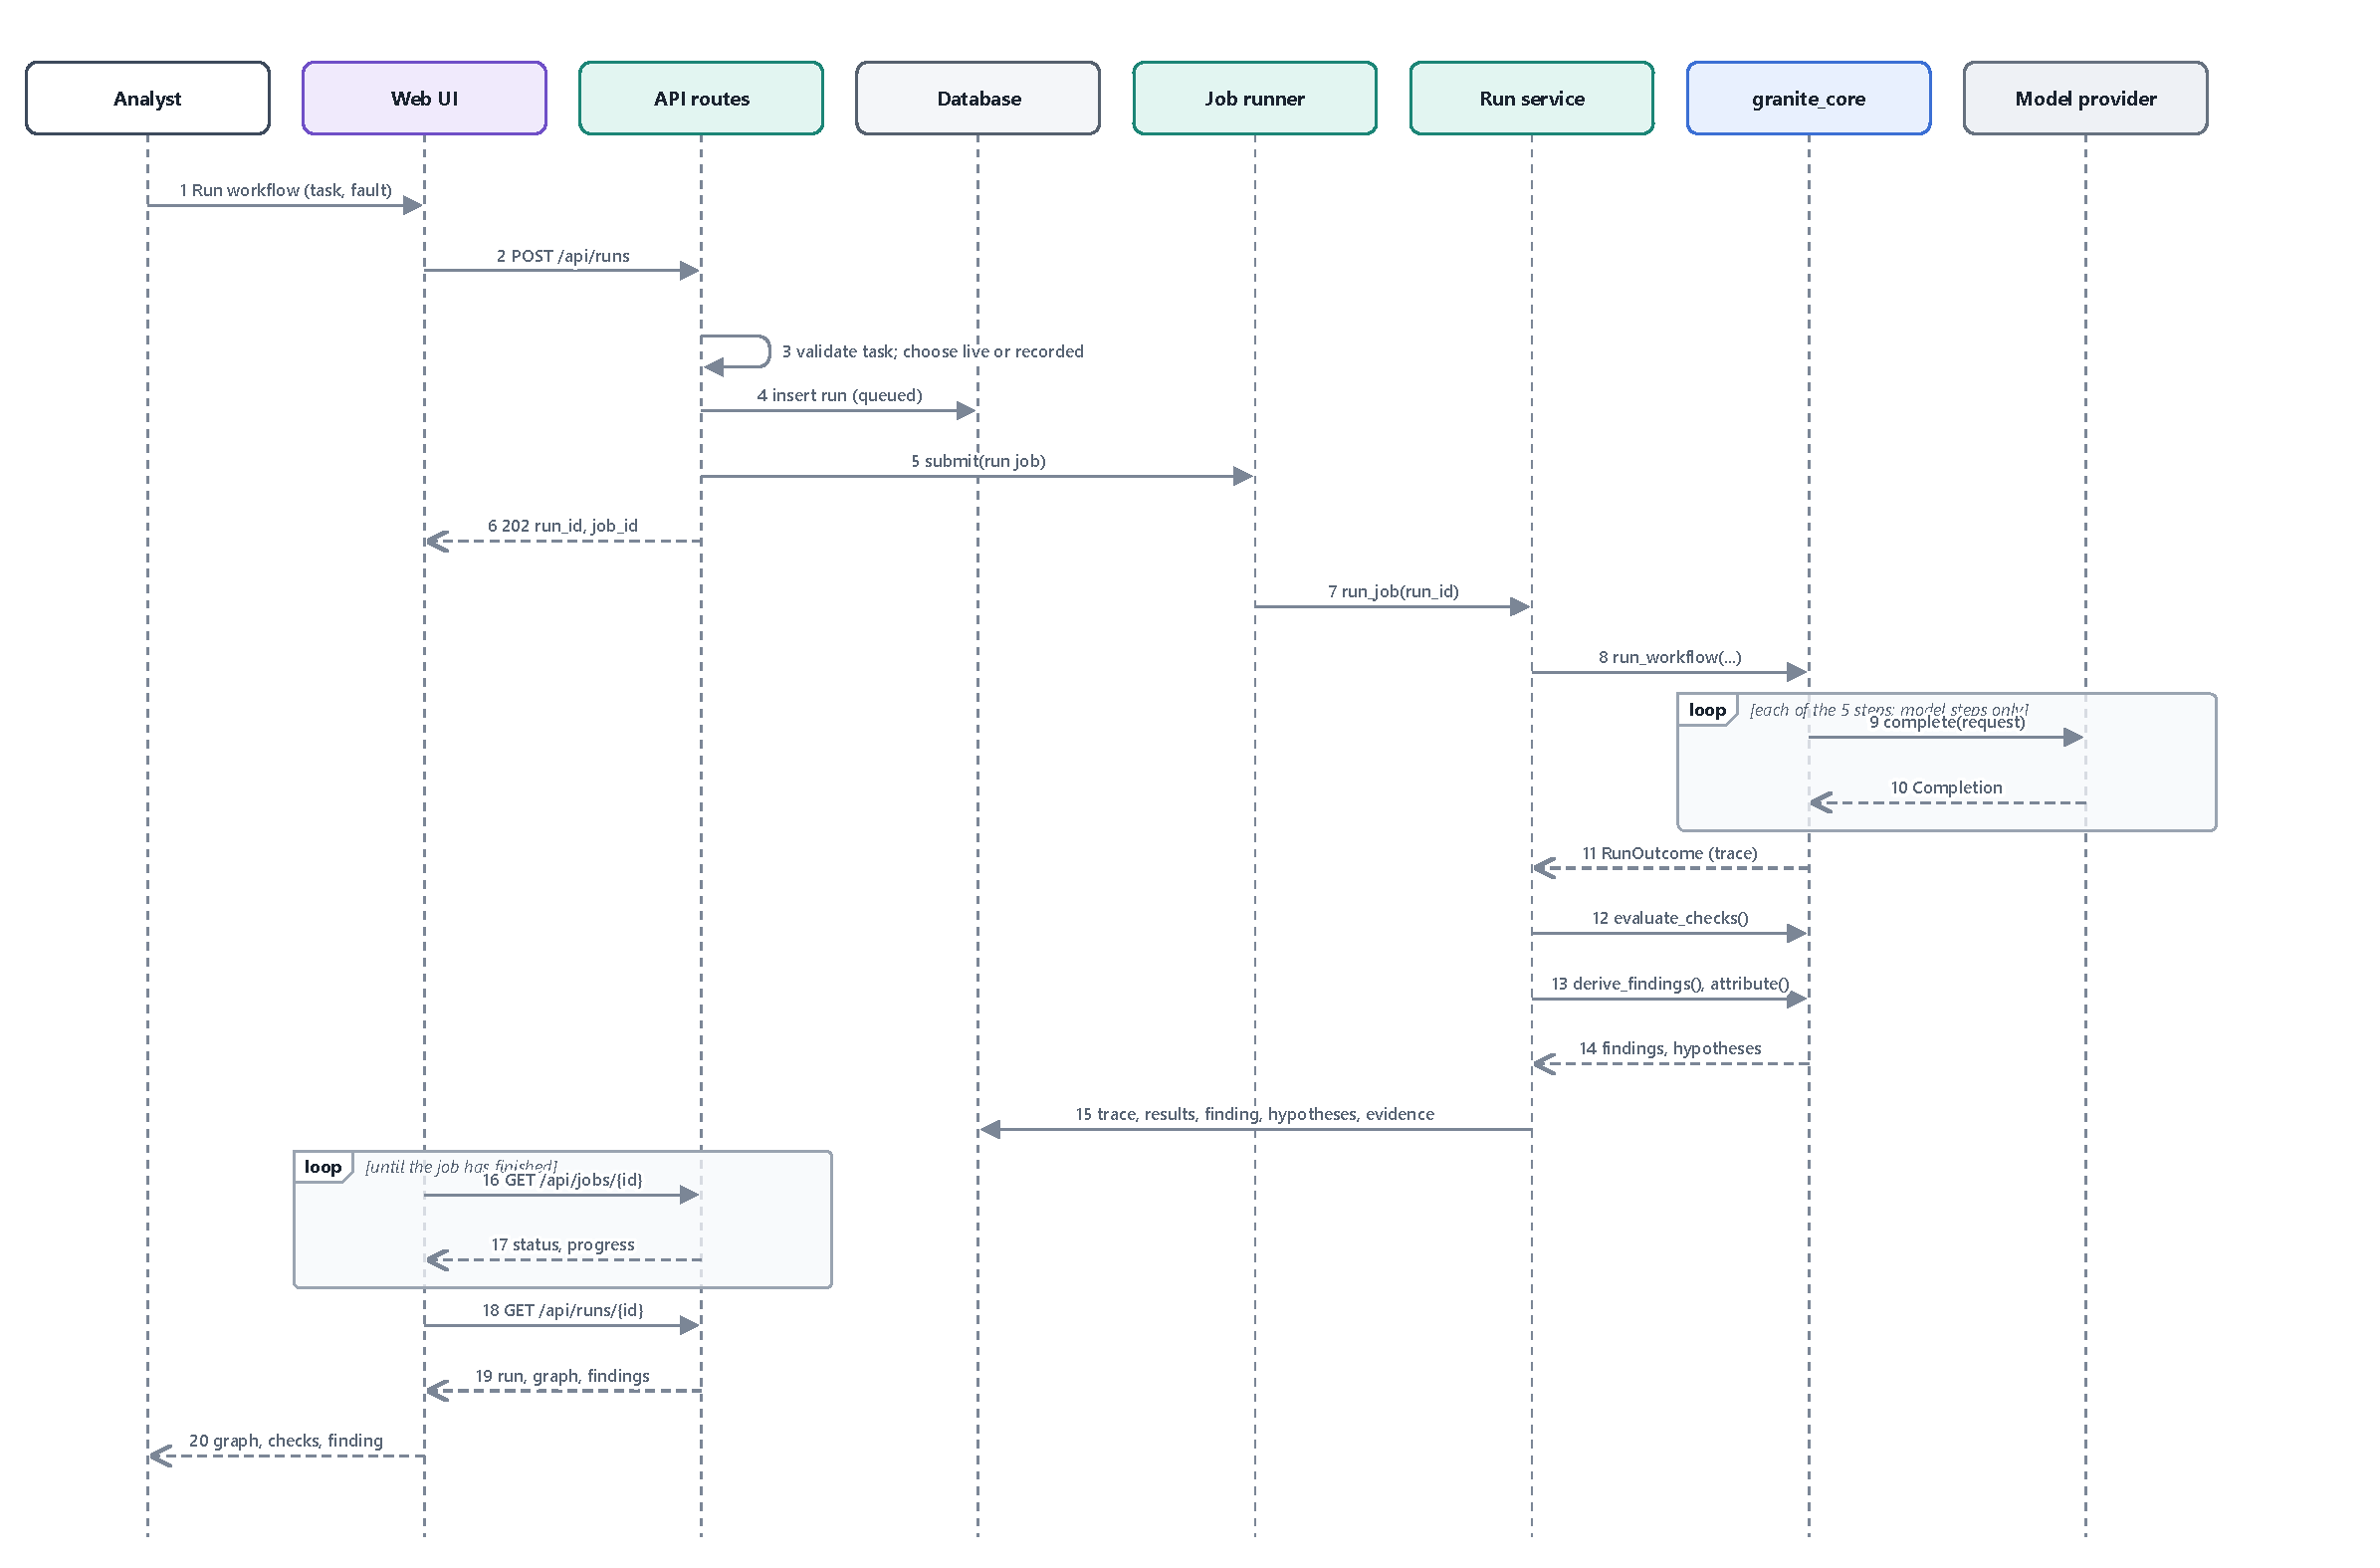
\includegraphics[width=\linewidth,height=0.42\textheight,keepaspectratio]{run-sequence.pdf}
\caption{System sequence for UC-03, running a workflow}
\label{fig:run-sequence}
\end{figure}


\begin{figure}[htbp]
\centering
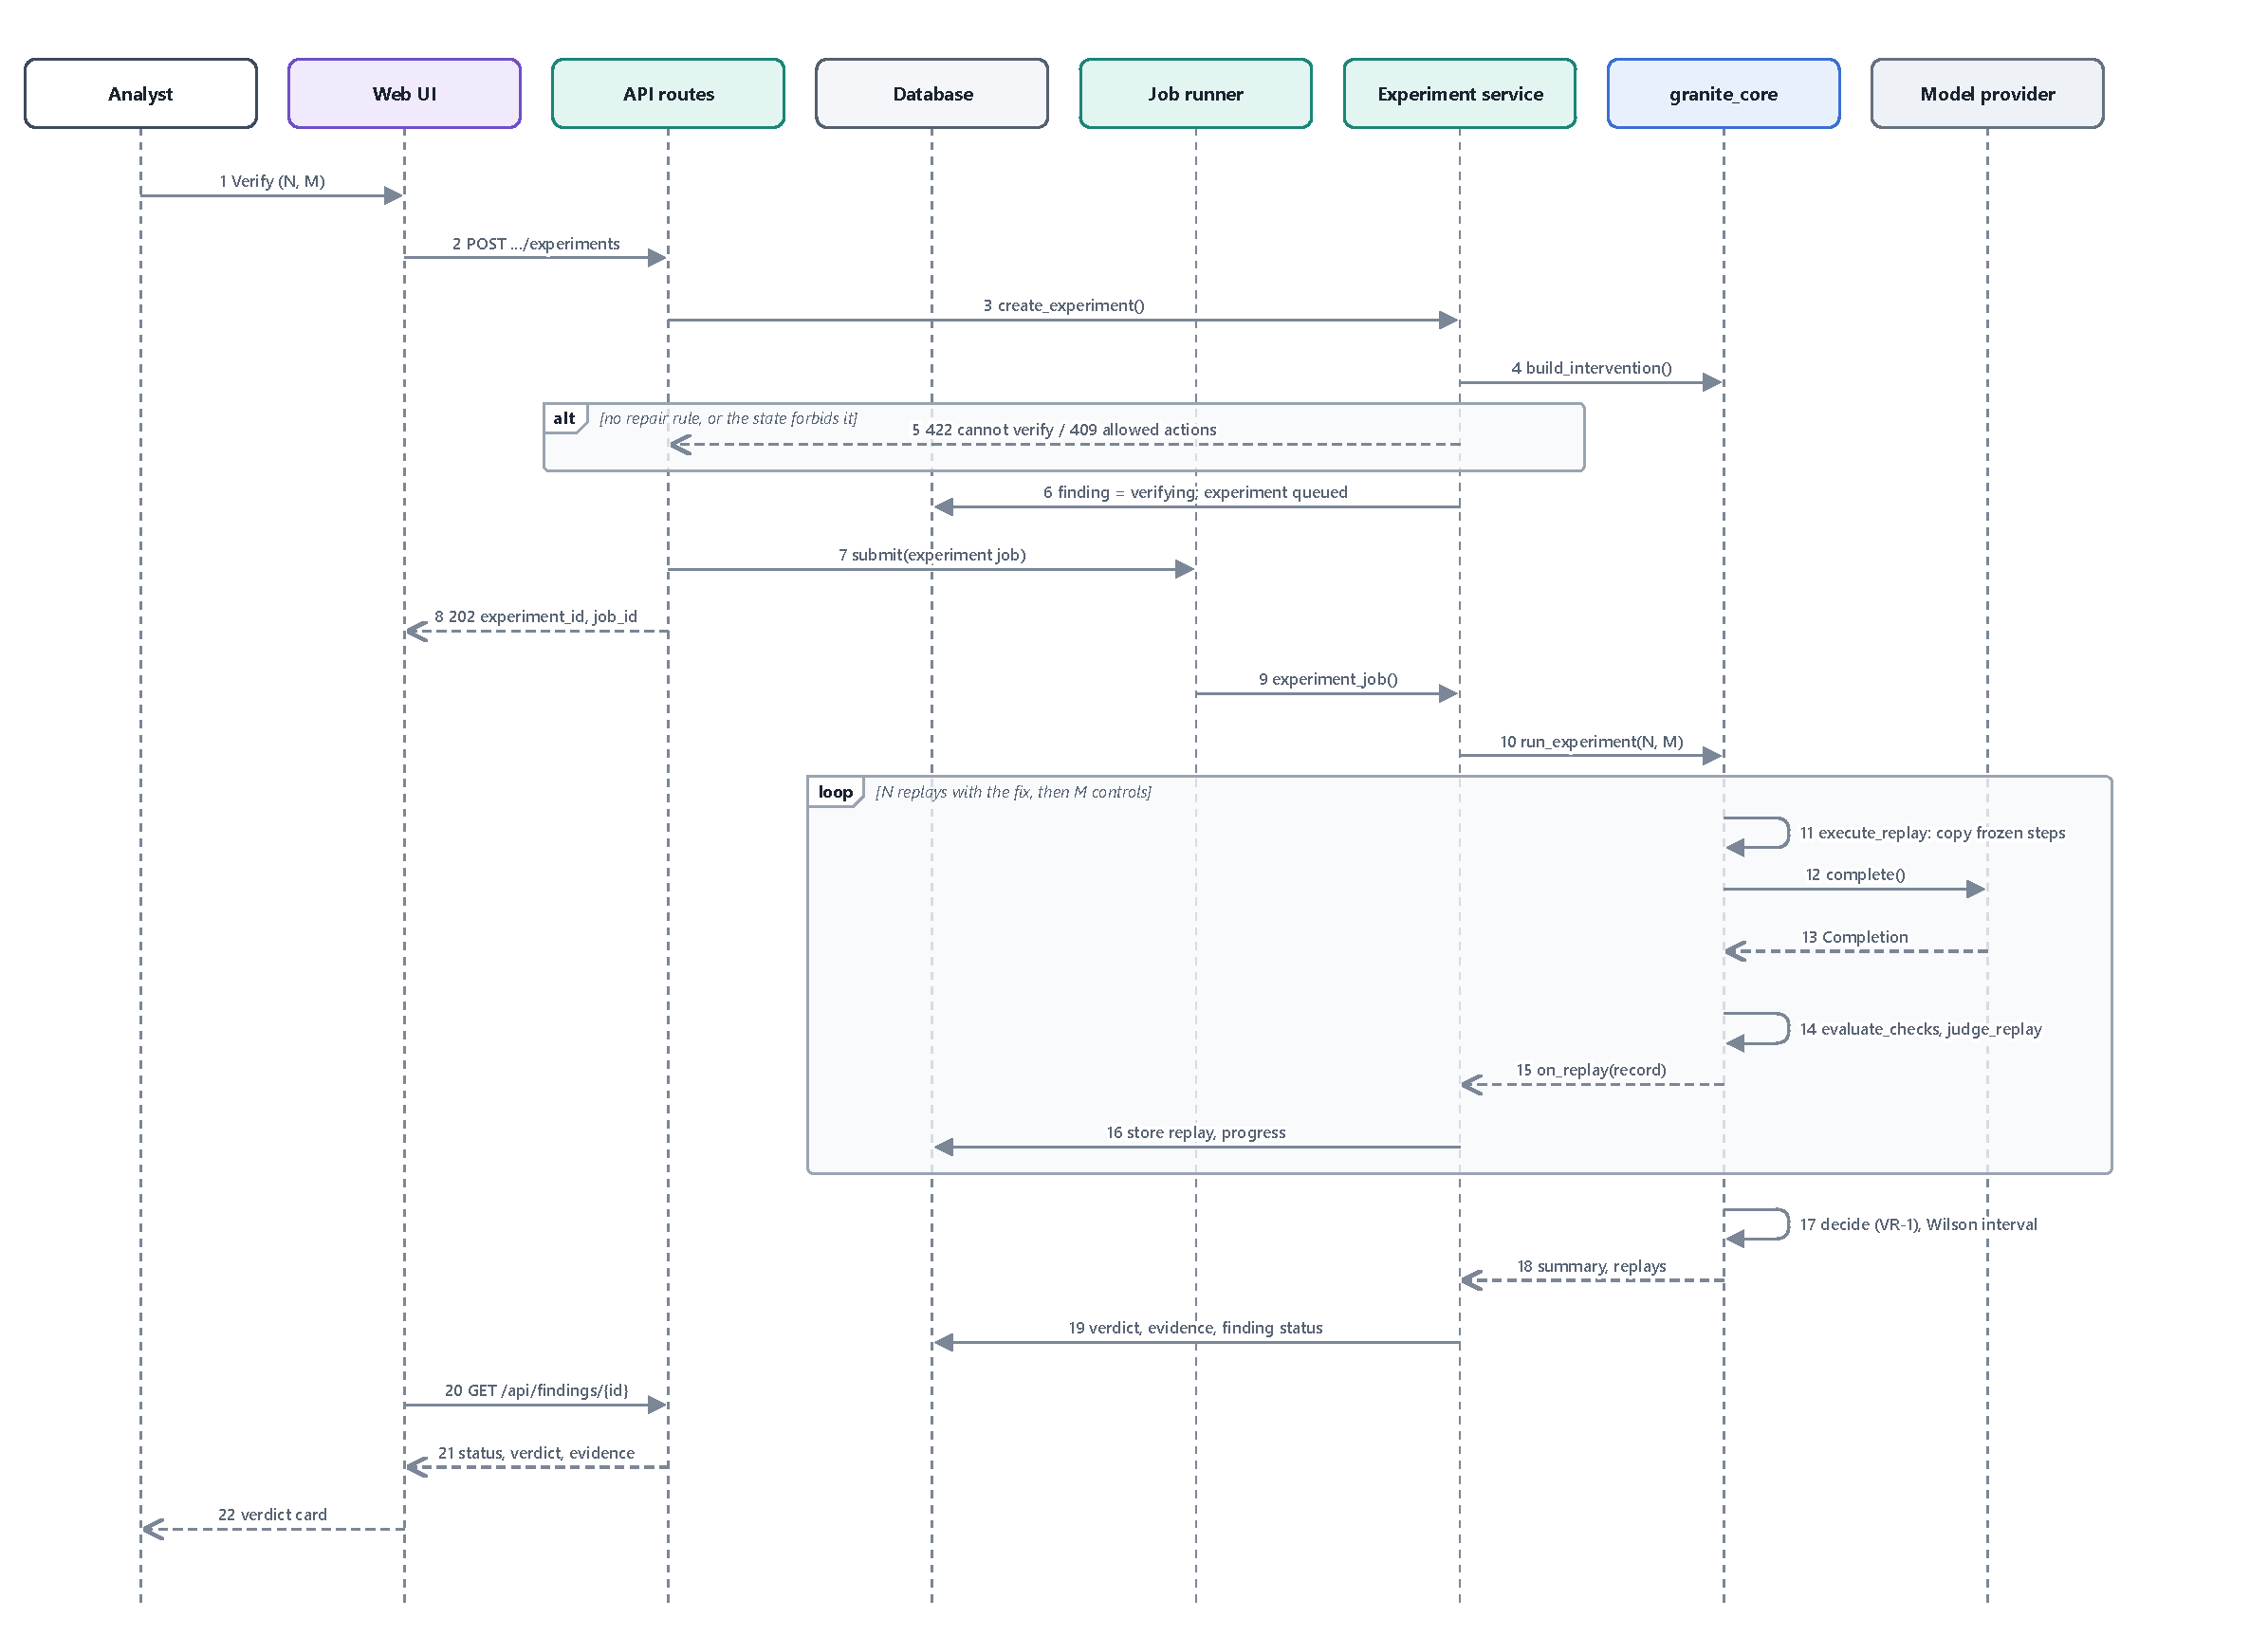
\includegraphics[width=\linewidth,height=0.42\textheight,keepaspectratio]{verification-sequence.pdf}
\caption{System sequence for UC-08, verifying a hypothesis by controlled replay}
\label{fig:verification-sequence-uc}
\end{figure}


\section{Functional Requirements}

The functional requirements below are grouped by product module. Each has an identifier, a priority (M Must, S Should), a testable acceptance criterion and its status at Mid-1. Requirements planned for later milestones are listed in Appendix B.

\subsection{Module 1: Run}

{\small
\begin{longtable}{>{\raggedright\arraybackslash\hspace{0pt}}p{0.062\linewidth}>{\raggedright\arraybackslash\hspace{0pt}}p{0.320\linewidth}>{\raggedright\arraybackslash\hspace{0pt}}p{0.027\linewidth}>{\raggedright\arraybackslash\hspace{0pt}}p{0.320\linewidth}>{\raggedright\arraybackslash\hspace{0pt}}p{0.101\linewidth}}
\caption{Module 1: Run}\label{tab:chapter4_requirements-2}\\
\toprule
\textbf{ID} & \textbf{Requirement} & \textbf{Pri.} & \textbf{Acceptance criterion} & \textbf{Status} \\
\midrule
\endfirsthead
\toprule
\textbf{ID} & \textbf{Requirement} & \textbf{Pri.} & \textbf{Acceptance criterion} & \textbf{Status} \\
\midrule
\endhead
\bottomrule
\endlastfoot
FR-RUN-01 & Execute the Refund Desk workflow from a validated input form and record every step's inputs, outputs, model, parameters and timings & M & A valid run yields 5 steps with inputs, outputs and timestamps & Done \\
FR-RUN-02 & Let the user enable a named fault and record its ground truth without exposing it to attribution & M & Fault record exists; attribution has no read path to it (test) & Done \\
FR-RUN-03 & Support live and recorded model modes; recorded mode replays cached answers & M & Same input in recorded mode gives byte-identical outputs across 3 runs & Done \\
FR-RUN-04 & Mark a run errored with an actionable message when the model is unreachable or times out & M & Closed port ends errored within 35 s; UI shows message and retry & Done (timeout 120 s for local models, deviation C-02g) \\
\end{longtable}
}

\subsection{Module 2: Check}

{\small
\begin{longtable}{>{\raggedright\arraybackslash\hspace{0pt}}p{0.069\linewidth}>{\raggedright\arraybackslash\hspace{0pt}}p{0.348\linewidth}>{\raggedright\arraybackslash\hspace{0pt}}p{0.028\linewidth}>{\raggedright\arraybackslash\hspace{0pt}}p{0.295\linewidth}>{\raggedright\arraybackslash\hspace{0pt}}p{0.090\linewidth}}
\caption{Module 2: Check}\label{tab:chapter4_requirements-3}\\
\toprule
\textbf{ID} & \textbf{Requirement} & \textbf{Pri.} & \textbf{Acceptance criterion} & \textbf{Status} \\
\midrule
\endfirsthead
\toprule
\textbf{ID} & \textbf{Requirement} & \textbf{Pri.} & \textbf{Acceptance criterion} & \textbf{Status} \\
\midrule
\endhead
\bottomrule
\endlastfoot
FR-CHK-01 & Evaluate all checks on every run; store pass/fail/abstain/error with observed and expected values & M & Fault run fails the outcome check with both values & Done \\
FR-CHK-02 & Evaluate check expressions with a whitelisted syntax-tree evaluator; reject disallowed constructs & M & The malicious-expression set is rejected (25 tested; 15 required) & Done \\
FR-CHK-03 & Missing referenced fields yield ABSTAIN, never PASS & M & Test with a missing field abstains & Done \\
FR-CHK-04 & A completed run with a failing outcome check creates a silent-failure finding & M & Exactly one finding on the stale-price run & Partly (one finding per failing check, C-02h) \\
FR-CHK-06 & Truth checks query source-of-truth functions on a pinned data snapshot and store query and answer as evidence & M & Evidence holds query, response and snapshot version & Done \\
\end{longtable}
}

\subsection{Module 3: Trace back}

{\small
\begin{longtable}{>{\raggedright\arraybackslash\hspace{0pt}}p{0.060\linewidth}>{\raggedright\arraybackslash\hspace{0pt}}p{0.344\linewidth}>{\raggedright\arraybackslash\hspace{0pt}}p{0.031\linewidth}>{\raggedright\arraybackslash\hspace{0pt}}p{0.234\linewidth}>{\raggedright\arraybackslash\hspace{0pt}}p{0.161\linewidth}}
\caption{Module 3: Trace back}\label{tab:chapter4_requirements-4}\\
\toprule
\textbf{ID} & \textbf{Requirement} & \textbf{Pri.} & \textbf{Acceptance criterion} & \textbf{Status} \\
\midrule
\endfirsthead
\toprule
\textbf{ID} & \textbf{Requirement} & \textbf{Pri.} & \textbf{Acceptance criterion} & \textbf{Status} \\
\midrule
\endhead
\bottomrule
\endlastfoot
FR-ATT-01 & Produce 1--5 ranked origin hypotheses per finding, each with score, rationale and evidence & M & Order Lookup ranked first in $\geq$ 95\% of 20 runs & Partly (10/10 measured; 20-run criterion not yet measured) \\
FR-ATT-02 & Compute scores from evidence weights and graph position, never from an LLM self-report & M & Same input gives byte-identical output & Done \\
\end{longtable}
}

\subsection{Module 4: Verify}

{\small
\begin{longtable}{>{\raggedright\arraybackslash\hspace{0pt}}p{0.070\linewidth}>{\raggedright\arraybackslash\hspace{0pt}}p{0.377\linewidth}>{\raggedright\arraybackslash\hspace{0pt}}p{0.033\linewidth}>{\raggedright\arraybackslash\hspace{0pt}}p{0.298\linewidth}>{\raggedright\arraybackslash\hspace{0pt}}p{0.051\linewidth}}
\caption{Module 4: Verify}\label{tab:chapter4_requirements-5}\\
\toprule
\textbf{ID} & \textbf{Requirement} & \textbf{Pri.} & \textbf{Acceptance criterion} & \textbf{Status} \\
\midrule
\endfirsthead
\toprule
\textbf{ID} & \textbf{Requirement} & \textbf{Pri.} & \textbf{Acceptance criterion} & \textbf{Status} \\
\midrule
\endhead
\bottomrule
\endlastfoot
FR-VER-01 & Run a verification experiment under VR-1: freeze upstream, apply one intervention, re-execute downstream N times plus M controls & M & Fixing the faulty step is CONFIRMED and controls stay broken & Done \\
FR-VER-02 & Compute the verdict with VR-1 and a Wilson 95\% interval; store the rule version & M & Table test over 20 (k, N, c, M) combinations & Done \\
FR-VER-03 & A replay that introduces a new failing check counts as not passing (regression guard) & M & Test with a new failure counts as fail & Done \\
\end{longtable}
}

\subsection{Module 5: Review, Report and History}

{\small
\begin{longtable}{>{\raggedright\arraybackslash\hspace{0pt}}p{0.070\linewidth}>{\raggedright\arraybackslash\hspace{0pt}}p{0.356\linewidth}>{\raggedright\arraybackslash\hspace{0pt}}p{0.029\linewidth}>{\raggedright\arraybackslash\hspace{0pt}}p{0.259\linewidth}>{\raggedright\arraybackslash\hspace{0pt}}p{0.116\linewidth}}
\caption{Module 5: Review, Report and History}\label{tab:chapter4_requirements-6}\\
\toprule
\textbf{ID} & \textbf{Requirement} & \textbf{Pri.} & \textbf{Acceptance criterion} & \textbf{Status} \\
\midrule
\endfirsthead
\toprule
\textbf{ID} & \textbf{Requirement} & \textbf{Pri.} & \textbf{Acceptance criterion} & \textbf{Status} \\
\midrule
\endhead
\bottomrule
\endlastfoot
FR-REV-01 & Accept, reject or request information with comments (mandatory for reject and for accepting an inconclusive finding); store reviewer and time & M & Reject without comment refused; decision stored & Done \\
FR-REV-02 & Finding transitions follow the state machine; illegal ones are rejected; every transition is audited & M & Accept before verification refused (409) & Done \\
FR-REP-01 & Export a finding report in Markdown and JSON with evidence hashes (PDF at Final-1) & S & Report downloads with hashes & Partly (PDF at Final-1) \\
FR-HIS-01 & List runs and findings with filters and search, 25 per page & M & Filters by status, severity, level, date, text & Partly (no project filter; one project) \\
FR-SEC-01 & Redact personal data before storing step inputs and outputs & S & No seeded PII in the database after a run & Not met (D-07) \\
\end{longtable}
}

Requirements for Iteration 2 and FYP-2 (import, SDK, check editor, fix suggestion, recovered run, regression export, Fault Lab, evaluation, authentication, retention) are listed in Appendix B.

\section{Non-Functional Requirements}

The non-functional requirements define measurable qualities that the system must have. Each is stated with a target and the way it is measured; the status at Mid-1 is noted where it has been checked.

\subsection{Reliability}

NFR-04: no unhandled exception reaches the user; the named failure modes (model down, model timeout, malformed input, check error, database unavailable, partial replay) each end in a documented state. At Mid-1, model down, unrecorded task, illegal transitions, limits and restart recovery are covered by system tests SYS-ERR-01 to 07 and SYS-REL-01 to 03. NFR-05: deterministic components (checks, attribution, verdict) give byte-identical output on re-evaluation, checked by golden-file tests.

\subsection{Usability}

NFR-09: SUS score of at least 68 and at least 80\% of core-journey tasks completed without help (pilot with 3 participants at Final-1; protocol ready). NFR-10: WCAG 2.2 AA, with contrast of at least 4.5:1, a full keyboard path through the core journey and status never shown by colour alone; automated axe-core checks pass on every screen in light and dark themes.

\subsection{Performance}

NFR-01: checks and attribution for a run of up to 50 steps complete with a 95th percentile of at most 2 seconds. NFR-02: a VR-1 verification with N = 5 and M = 2 completes within 3 minutes with a hosted model (a local 3B model on a CPU is reported, not targeted). NFR-03: first contentful paint within 3 seconds after the server wakes; interactions within 200 ms.

\subsection{Security}

NFR-07: zero high or critical findings from bandit, pip-audit, npm audit and gitleaks on \texttt{main} (met); the check language rejects every expression in the malicious set (met); input and upload limits are enforced (met). NFR-08: no unredacted personal data in the database after a run (not yet met; synthetic data only on the public demo).

\subsection{Other qualities}

NFR-11 maintainability: core library line coverage of at least 80\% (measured 97.5\%), lint and strict type checks clean, complexity limit enforced. NFR-12 portability: \texttt{docker compose up} on a clean machine reaches a working interface within 15 minutes following the setup manual, verified by a non-owner (Final-1). NFR-13 availability: health checks green at evaluation time, with a warm-up before demos. NFR-14 cost: zero recurring cost.

\section{Acceptance Criteria}

{\small
\begin{longtable}{>{\raggedright\arraybackslash\hspace{0pt}}p{0.086\linewidth}>{\raggedright\arraybackslash\hspace{0pt}}p{0.494\linewidth}>{\raggedright\arraybackslash\hspace{0pt}}p{0.215\linewidth}>{\raggedright\arraybackslash\hspace{0pt}}p{0.065\linewidth}}
\caption{Acceptance Criteria}\label{tab:chapter4_requirements-7}\\
\toprule
\textbf{Feature} & \textbf{Acceptance check} & \textbf{Verified by} & \textbf{Result} \\
\midrule
\endfirsthead
\toprule
\textbf{Feature} & \textbf{Acceptance check} & \textbf{Verified by} & \textbf{Result} \\
\midrule
\endhead
\bottomrule
\endlastfoot
Run & A valid example run completes with 5 recorded steps and a trace hash & SYS-CORE-01, test\_runner & Pass \\
Detect & The stale-price run (one failing outcome check) opens one silent-failure finding; a clean run opens none & SYS-CORE-01, SYS-CORE-02 & Pass \\
Trace back & Order Lookup is ranked first with a truth-mismatch reason & SYS-CORE-01, feasibility M3 (10/10) & Pass \\
Verify & Verifying Order Lookup gives CONFIRMED (5/5 fixed, 0/2 controls); verifying the calculator gives REFUTED & SYS-CORE-03, feasibility M4/M5 & Pass \\
Review & Accept before verification is refused; reject needs a comment; decisions are recorded & SYS-ERR-03 & Pass \\
Evidence & Evidence is append-only and hashes match; ground truth never appears in evidence & SYS-SEC-02, SYS-SEC-03 & Pass \\
Errors & Invalid input refused per field; model down ends errored with a reason & SYS-ERR-01, SYS-ERR-07 & Pass \\
History & Runs and findings can be found again with filters & SYS-CORE-05 & Pass \\
\end{longtable}
}

\section{Requirements Traceability}

{\small
\begin{longtable}{>{\raggedright\arraybackslash\hspace{0pt}}p{0.096\linewidth}>{\raggedright\arraybackslash\hspace{0pt}}p{0.182\linewidth}>{\raggedright\arraybackslash\hspace{0pt}}p{0.265\linewidth}>{\raggedright\arraybackslash\hspace{0pt}}p{0.316\linewidth}}
\caption{Requirements Traceability}\label{tab:chapter4_requirements-8}\\
\toprule
\textbf{Requirement} & \textbf{Design element} & \textbf{Implementation} & \textbf{Test} \\
\midrule
\endfirsthead
\toprule
\textbf{Requirement} & \textbf{Design element} & \textbf{Implementation} & \textbf{Test} \\
\midrule
\endhead
\bottomrule
\endlastfoot
FR-RUN-01 & Runner, Trace v1 & \texttt{runner.\allowbreak{}py::run\_\allowbreak{}workflow}, \texttt{refund\_\allowbreak{}desk/\allowbreak{}definition.\allowbreak{}py} & \texttt{test\_\allowbreak{}runner.\allowbreak{}py}, \texttt{test\_\allowbreak{}journeys.\allowbreak{}py} \\
FR-RUN-02 & Fault record hidden from analysis & \texttt{faults.\allowbreak{}py::StalePriceFault} & \texttt{test\_\allowbreak{}attribution\_\allowbreak{}never\_\allowbreak{}sees\_\allowbreak{}fault\_\allowbreak{}ground\_\allowbreak{}truth} \\
FR-RUN-03 & Provider layer, cassette & \texttt{llm.\allowbreak{}py::RecordedProvider} & \texttt{test\_\allowbreak{}fr\_\allowbreak{}run\_\allowbreak{}03\_\allowbreak{}recorded\_\allowbreak{}mode\_\allowbreak{}gives\_\allowbreak{}byte\_\allowbreak{}identical\ldots{}} \\
FR-CHK-02 & Check language (ADR-004) & \texttt{dsl.\allowbreak{}py::compile\_\allowbreak{}expression} & \texttt{test\_\allowbreak{}dsl.\allowbreak{}py::test\_\allowbreak{}malicious\_\allowbreak{}expressions\_\allowbreak{}are\_\allowbreak{}rejected} \\
FR-CHK-03 & Check results & \texttt{checks.\allowbreak{}py::evaluate\_\allowbreak{}check} & \texttt{test\_\allowbreak{}missing\_\allowbreak{}field\_\allowbreak{}abstains\_\allowbreak{}never\_\allowbreak{}passes} \\
FR-ATT-01/02 & Provenance attribution (ADR-005) & \texttt{attribution.\allowbreak{}py::attribute} & \texttt{test\_\allowbreak{}attribution.\allowbreak{}py}, \texttt{test\_\allowbreak{}attribution\_\allowbreak{}ranks\_\allowbreak{}the\_\allowbreak{}injected\_\allowbreak{}step\_\allowbreak{}first\ldots{}} \\
FR-VER-01/02 & VR-1 (ADR-006), replay plan & \texttt{verification.\allowbreak{}py::decide}, \texttt{experiment.\allowbreak{}py::run\_\allowbreak{}experiment} & \texttt{test\_\allowbreak{}verification.\allowbreak{}py}, \texttt{test\_\allowbreak{}experiment.\allowbreak{}py} \\
FR-REV-01/02 & Finding state machine & \texttt{lifecycle.\allowbreak{}py::transition}, \texttt{services/\allowbreak{}reviews.\allowbreak{}py} & \texttt{test\_\allowbreak{}lifecycle\_\allowbreak{}\ldots{}}, SYS-ERR-03 \\
FR-REP-01 & Report service & \texttt{services/\allowbreak{}report.\allowbreak{}py} & \texttt{test\_\allowbreak{}journeys.\allowbreak{}py} \\
\end{longtable}
}

The full matrix for all 19 Mid-1 requirements is generated from the code by \texttt{scripts/\allowbreak{}check\_\allowbreak{}traceability.\allowbreak{}py} (\texttt{docs/\allowbreak{}plan/\allowbreak{}requirements-trace.\allowbreak{}md}); see Appendix B.

%======================================================================================
% chapter5_design
%======================================================================================
\chapter{System Design}

This chapter describes Granite's design: the layered architecture and its components, the interfaces between them, the main architecture decisions and their rationale, how the design evolved since the proposal, and the domain, data and behaviour models. All diagrams are generated from the code, so they match the implementation.

\section{System Architecture}

Granite is a modular monolith: one repository, four packages and one direction of dependency. The web interface (React) talks to the API over HTTP; the API (FastAPI) stores data, runs background jobs and calls the workflow and the core library; the Refund Desk workflow depends only on the core; and the core library (\texttt{granite\_\allowbreak{}core}) contains the trace model, runner, check language, checks, attribution, verification, lifecycle and evidence logic with no web, database or network code. Because the core imports only the Python standard library and Pydantic, its algorithms can be tested on their own in seconds, and a script in CI fails the build if a forbidden import appears. External services (the language-model provider and the database) are reached only through the API layer.

{\small
\begin{longtable}{>{\raggedright\arraybackslash\hspace{0pt}}p{0.153\linewidth}>{\raggedright\arraybackslash\hspace{0pt}}p{0.218\linewidth}>{\raggedright\arraybackslash\hspace{0pt}}p{0.224\linewidth}>{\raggedright\arraybackslash\hspace{0pt}}p{0.266\linewidth}}
\caption{System Architecture}\label{tab:chapter5_design-1}\\
\toprule
\textbf{Layer} & \textbf{Package} & \textbf{May import} & \textbf{Must not import} \\
\midrule
\endfirsthead
\toprule
\textbf{Layer} & \textbf{Package} & \textbf{May import} & \textbf{Must not import} \\
\midrule
\endhead
\bottomrule
\endlastfoot
Presentation & \texttt{apps/\allowbreak{}web} & the API over HTTP & anything else \\
Application & \texttt{apps/\allowbreak{}api} (\texttt{granite\_\allowbreak{}api}) & core, workflow, FastAPI, SQLAlchemy & UI code \\
Workflow under test & \texttt{workflows/\allowbreak{}refund\_\allowbreak{}desk} & core & API, web or database libraries \\
Domain core & \texttt{packages/\allowbreak{}granite\_\allowbreak{}core} & standard library, Pydantic & FastAPI, SQLAlchemy, HTTP clients, any workflow \\
\end{longtable}
}

Figure~\ref{fig:layers} shows the layers and the direction of dependency.

\begin{figure}[htbp]
\centering
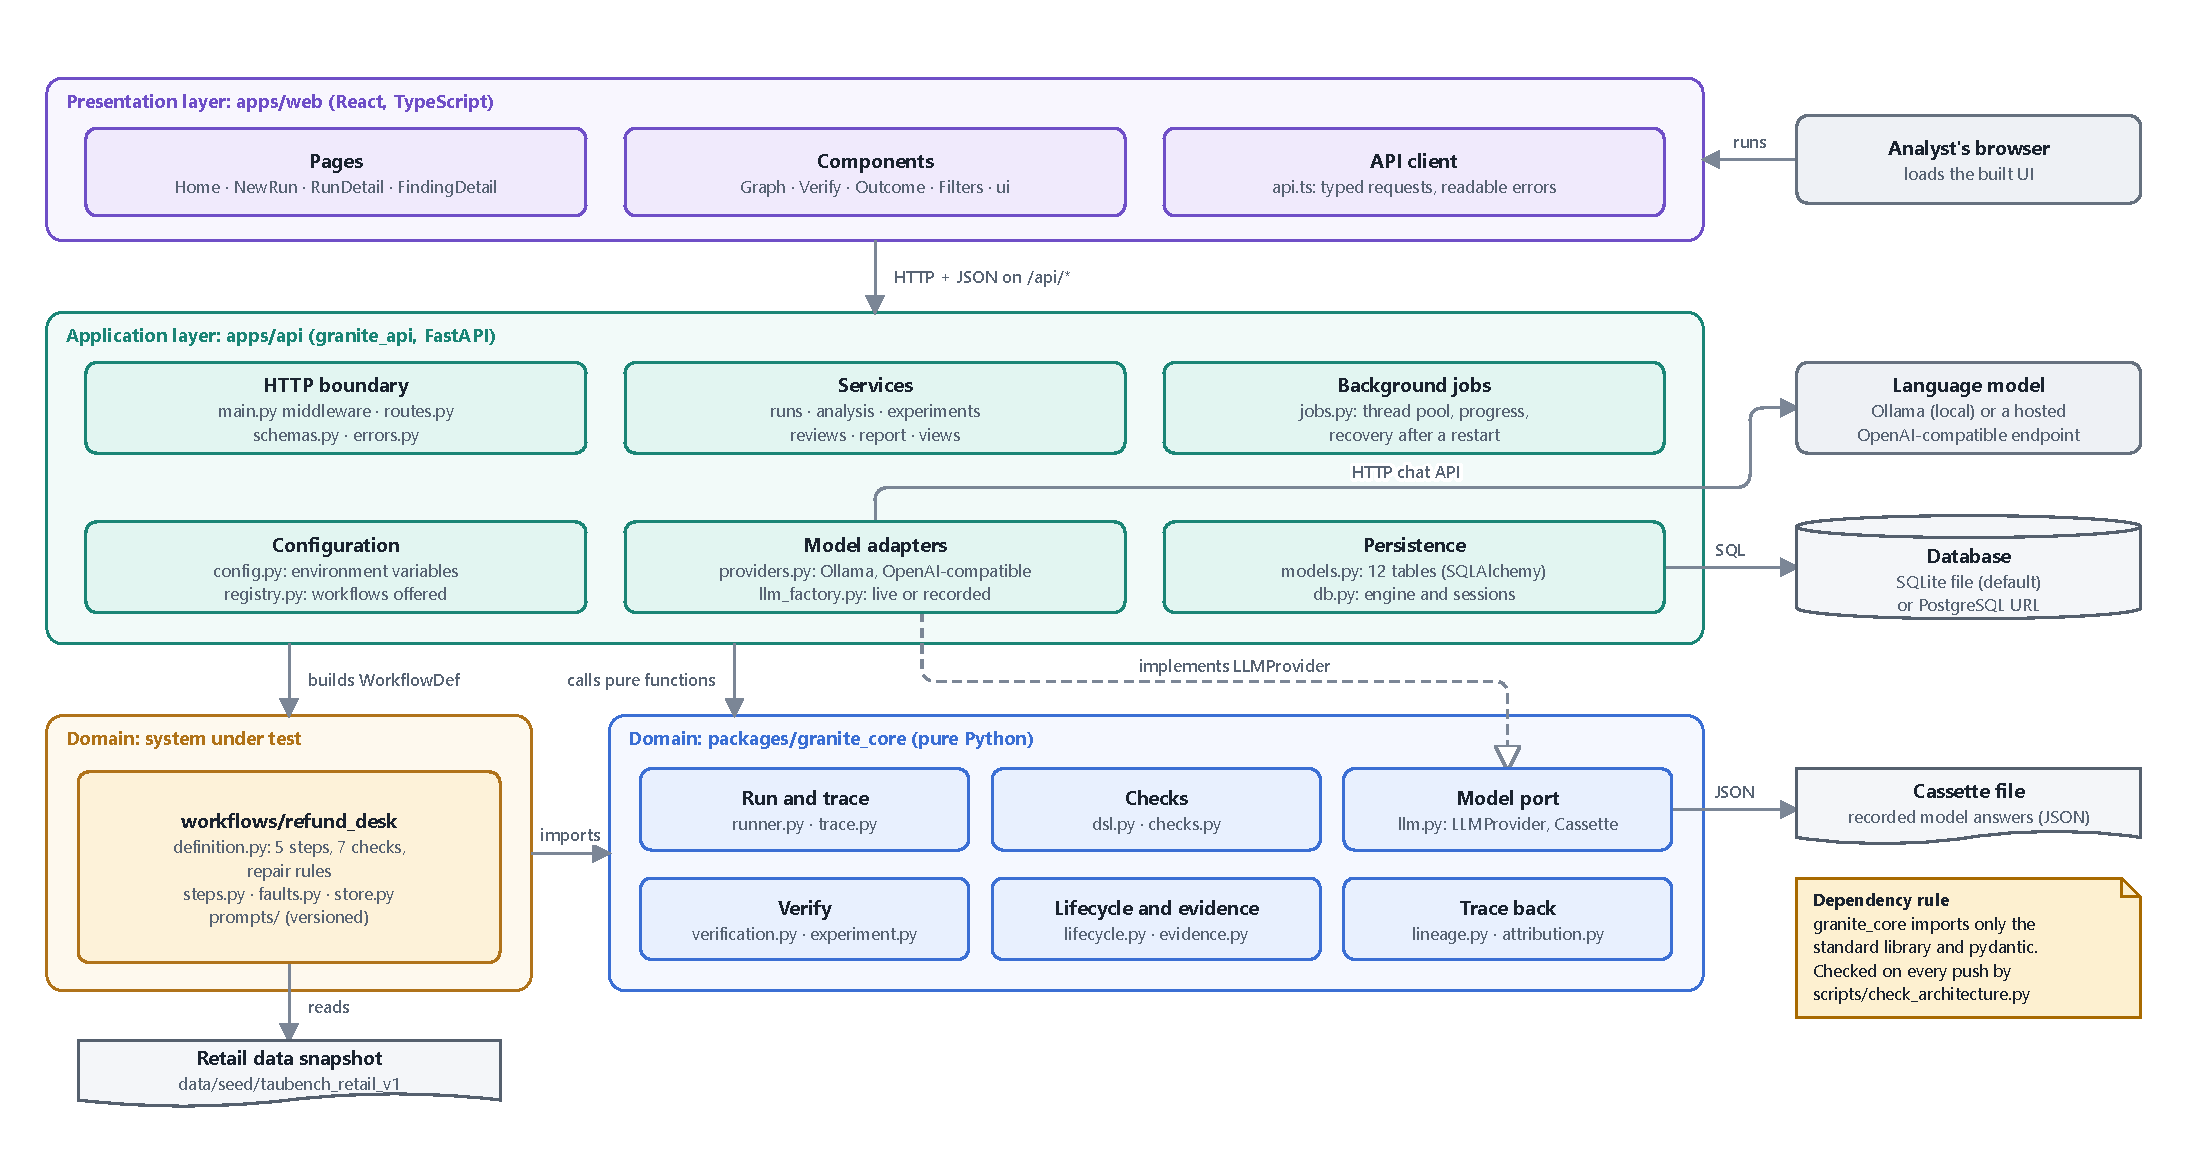
\includegraphics[width=\linewidth,height=0.42\textheight,keepaspectratio]{layer-diagram.pdf}
\caption{Layer diagram: one dependency direction, checked in CI}
\label{fig:layers}
\end{figure}


\section{Architectural Components}

\textbf{Web interface} (\texttt{apps/\allowbreak{}web}): five screens (Investigations, New run, Run, Finding, How it works), a keyboard-operable pipeline graph, the verification table and the review panel. \textbf{API} (\texttt{granite\_\allowbreak{}api}): sixteen HTTP endpoints, request validation, RFC 7807 error responses, security headers, a body-size limit, rate limiting and an optional access token. \textbf{Services}: one per use case (runs, analysis, experiments, reviews, report). \textbf{Job runner}: a thread pool with a job table, so long runs and replays do not block requests, and interrupted jobs are marked failed on restart. \textbf{Persistence}: SQLAlchemy over SQLite (PostgreSQL supported). \textbf{Provider layer}: live (Ollama or an OpenAI-compatible endpoint), recorded (cassette of real answers) or automatic. \textbf{Core library}: trace, runner, check language (DSL), checks, lineage, attribution, verification, experiment, lifecycle, evidence, redaction. \textbf{Refund Desk}: five steps, seven checks, repair rules, the stale-price fault and an independent retail store used as the source of truth.

Figure~\ref{fig:components} shows these components and the interfaces between them.

\begin{figure}[htbp]
\centering
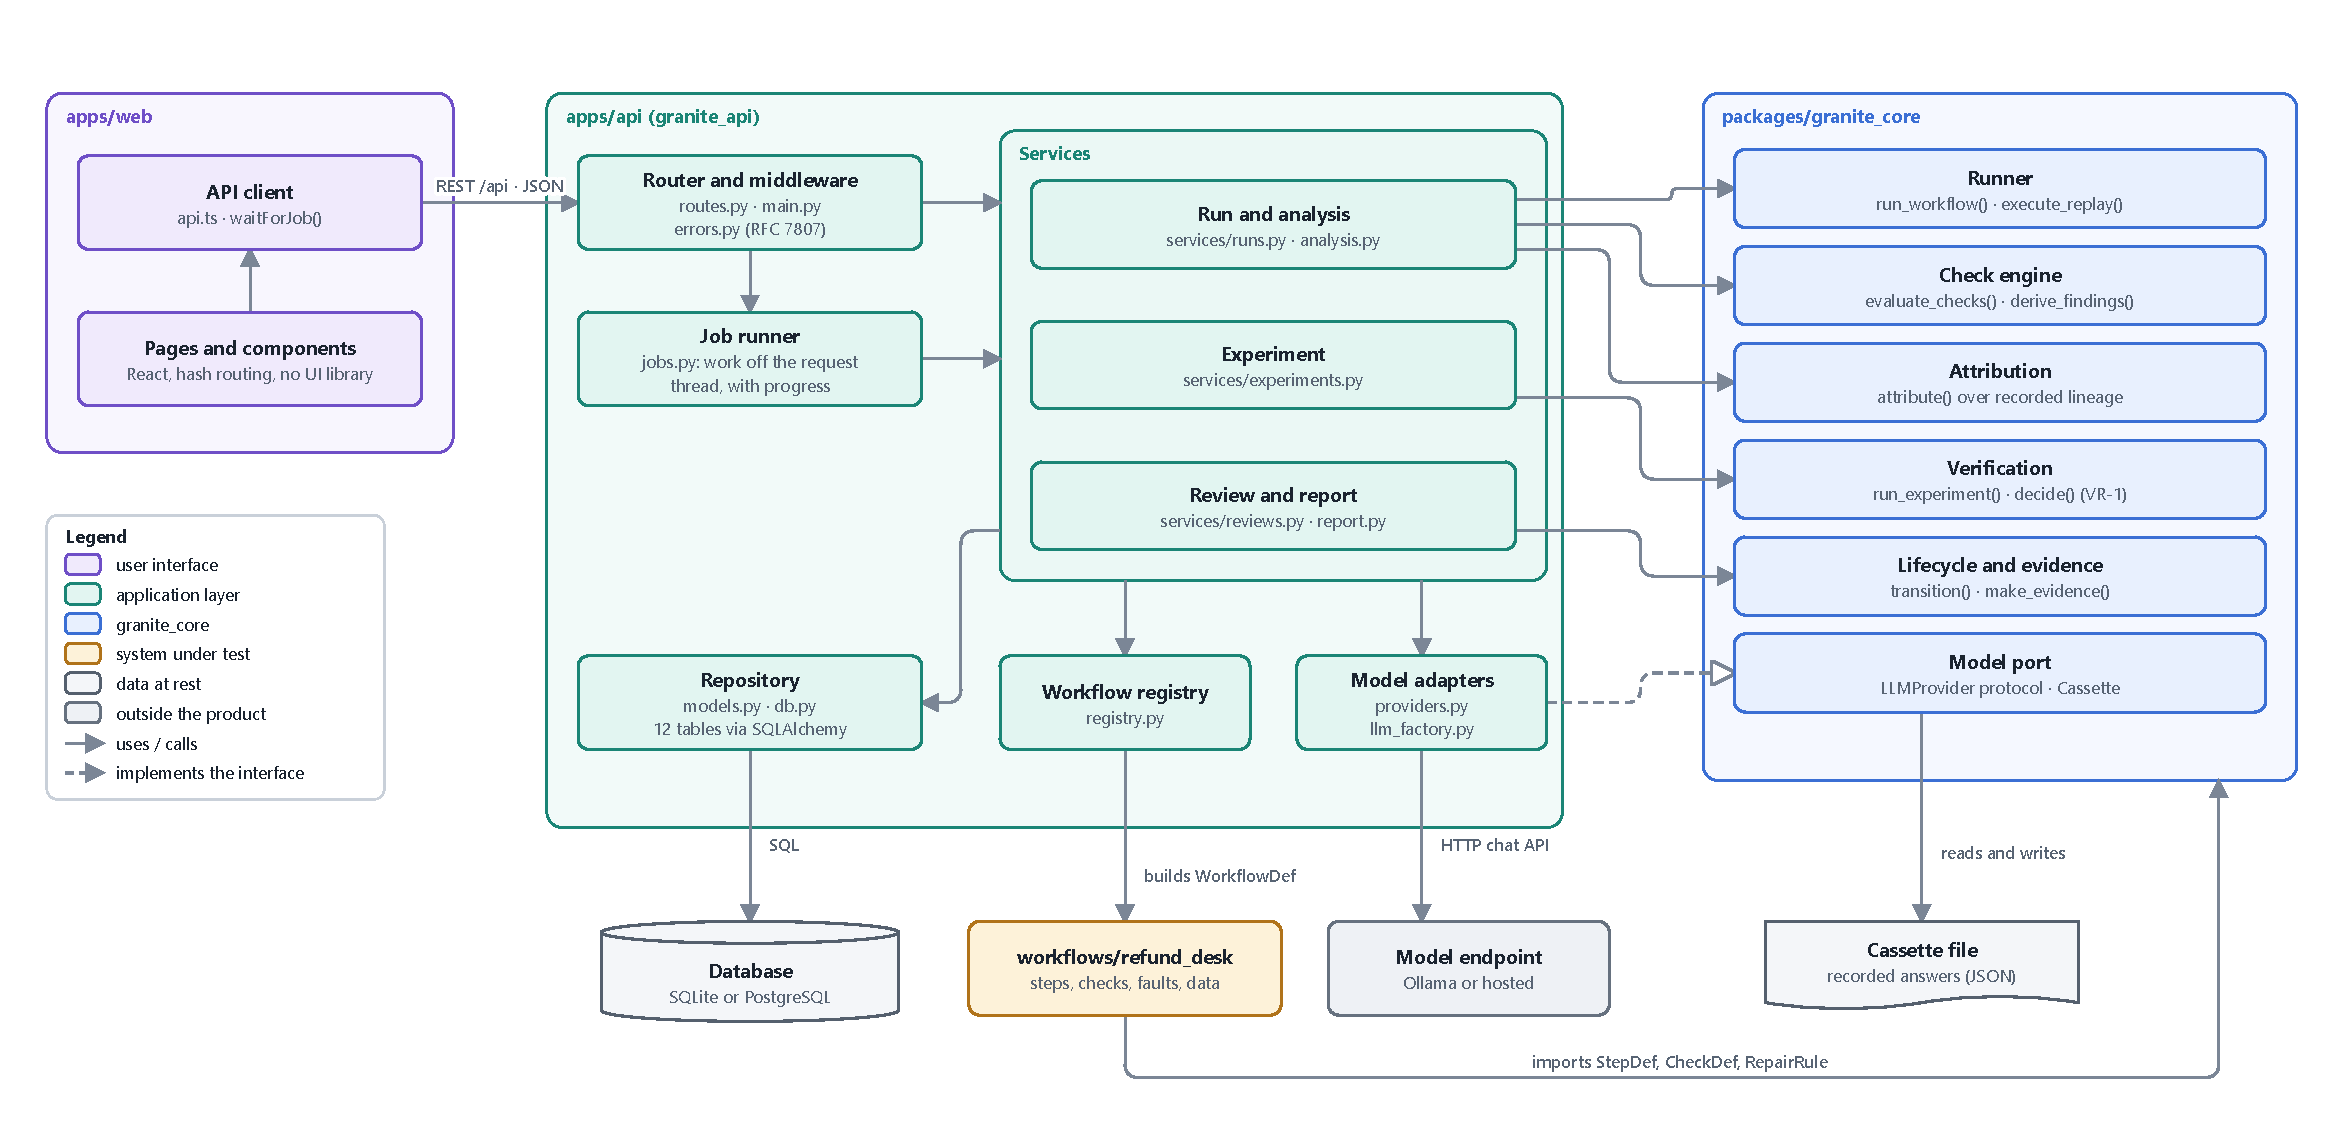
\includegraphics[width=\linewidth,height=0.42\textheight,keepaspectratio]{component-diagram.pdf}
\caption{Component diagram}
\label{fig:components}
\end{figure}


\section{Interfaces and Dependencies}

\textbf{HTTP API} (all under \texttt{/\allowbreak{}api}, documented automatically at \texttt{/\allowbreak{}docs}):

{\small
\begin{longtable}{>{\raggedright\arraybackslash\hspace{0pt}}p{0.346\linewidth}>{\raggedright\arraybackslash\hspace{0pt}}p{0.363\linewidth}>{\raggedright\arraybackslash\hspace{0pt}}p{0.181\linewidth}}
\caption{Interfaces and Dependencies}\label{tab:chapter5_design-2}\\
\toprule
\textbf{Method and path} & \textbf{Purpose} & \textbf{Main responses} \\
\midrule
\endfirsthead
\toprule
\textbf{Method and path} & \textbf{Purpose} & \textbf{Main responses} \\
\midrule
\endhead
\bottomrule
\endlastfoot
GET \texttt{/\allowbreak{}workflows}, \texttt{/\allowbreak{}workflows/\allowbreak{}\{key\}/\allowbreak{}examples} & Registered workflows and example tasks & 200 \\
POST \texttt{/\allowbreak{}runs} & Start a run (task, fault, seed, mode) & 202 with a job id; 422 invalid input; 429 rate limit \\
GET \texttt{/\allowbreak{}runs}, \texttt{/\allowbreak{}runs/\allowbreak{}\{id\}}, \texttt{/\allowbreak{}runs/\allowbreak{}\{id\}/\allowbreak{}graph} & List, detail (trace, checks, findings), data-flow graph & 200; 404 \\
GET \texttt{/\allowbreak{}findings}, \texttt{/\allowbreak{}findings/\allowbreak{}summary}, \texttt{/\allowbreak{}findings/\allowbreak{}\{id\}} & List with filters, counts by status, detail with allowed actions & 200; 404 \\
GET \texttt{/\allowbreak{}findings/\allowbreak{}\{id\}/\allowbreak{}report?format=md|json} & Export the investigation & 200 \\
POST \texttt{/\allowbreak{}hypotheses/\allowbreak{}\{id\}/\allowbreak{}experiments} & Start a verification (N, M) & 202; 409 not allowed now \\
GET \texttt{/\allowbreak{}experiments/\allowbreak{}\{id\}} & Replays, summary and verdict & 200 \\
POST \texttt{/\allowbreak{}findings/\allowbreak{}\{id\}/\allowbreak{}reviews} & Record a decision & 201; 409 illegal transition; 422 missing comment \\
GET \texttt{/\allowbreak{}evidence/\allowbreak{}\{id\}} & One evidence record with hash check & 200 \\
GET \texttt{/\allowbreak{}jobs/\allowbreak{}\{id\}} & Job status and progress & 200 \\
POST \texttt{/\allowbreak{}settings/\allowbreak{}test-llm} & Check the model connection & 200 \\
\end{longtable}
}

\textbf{Internal contracts:} the core exposes \texttt{run\_\allowbreak{}workflow} and \texttt{execute\_\allowbreak{}replay} (runner), \texttt{evaluate\_\allowbreak{}checks} and \texttt{derive\_\allowbreak{}findings} (checks), \texttt{attribute} (attribution), \texttt{plan\_\allowbreak{}replay}, \texttt{decide} and \texttt{wilson} (verification), \texttt{run\_\allowbreak{}experiment} (experiment), \texttt{transition} (lifecycle), and \texttt{make\_\allowbreak{}evidence}/\texttt{verify\_\allowbreak{}evidence} (evidence). A workflow is described by a \texttt{WorkflowDef} (steps with declared reads, checks, repair rules and truth functions). Traces follow the published Granite Trace v1 JSON Schema. \textbf{External dependencies:} Ollama with llama3.2:3b (live mode), SQLite/PostgreSQL, Render (hosting), GitHub Actions and the Container Registry (CI/CD).

\section{Architecture Decisions and Rationale}

{\small
\begin{longtable}{>{\raggedright\arraybackslash\hspace{0pt}}p{0.038\linewidth}>{\raggedright\arraybackslash\hspace{0pt}}p{0.239\linewidth}>{\raggedright\arraybackslash\hspace{0pt}}p{0.338\linewidth}>{\raggedright\arraybackslash\hspace{0pt}}p{0.245\linewidth}}
\caption{Architecture Decisions and Rationale}\label{tab:chapter5_design-3}\\
\toprule
\textbf{ADR} & \textbf{Decision} & \textbf{Rationale} & \textbf{Alternatives rejected} \\
\midrule
\endfirsthead
\toprule
\textbf{ADR} & \textbf{Decision} & \textbf{Rationale} & \textbf{Alternatives rejected} \\
\midrule
\endhead
\bottomrule
\endlastfoot
001 & Modular monolith with one dependency direction & Simple to run, test and deploy for a three-person team; boundaries enforced by imports & Microservices (operational cost) \\
002 & Own workflow runner first & Full control of the trace and of replay from any step & Instrumenting CrewAI/LangGraph first (no replay control) \\
003 & SQLAlchemy persistence; one JSON trace document per run & One source for hashing and replay; fewer tables to keep consistent & Separate step and edge tables \\
004 & Check language on Python's syntax tree with a whitelist & Safe and explainable code we can defend & \texttt{eval} (unsafe); third-party evaluator \\
005 & Provenance-first attribution & Deterministic, cheap, testable; LLM opinion only as a labelled second opinion & LLM-judge attribution as the core \\
006 & Verdict rule VR-1 with controls & Separates real causes from model randomness; versioned thresholds & Single re-run; unversioned thresholds \\
007 & Free hosting on Render & Zero cost; Docker deploy & Paid hosting; Hugging Face Spaces (free tier changed) \\
008 & Provider abstraction and recorded mode & Demo and tests run offline and reproducibly & Calling a model on every run \\
009 & Granite Trace v1 schema & Stable input contract for import and SDK & Framework-specific formats \\
010 & Short-lived branches into \texttt{main} with pull requests & Reviewed, CI-checked changes; simple for a small team & Git-flow with \texttt{develop} (revised 11 Oct) \\
\end{longtable}
}

\section{Design Evolution}

{\small
\begin{longtable}{>{\raggedright\arraybackslash\hspace{0pt}}p{0.085\linewidth}>{\raggedright\arraybackslash\hspace{0pt}}p{0.199\linewidth}>{\raggedright\arraybackslash\hspace{0pt}}p{0.333\linewidth}>{\raggedright\arraybackslash\hspace{0pt}}p{0.243\linewidth}}
\caption{Design Evolution}\label{tab:chapter5_design-4}\\
\toprule
\textbf{Aspect} & \textbf{At the proposal} & \textbf{Now (Mid-1)} & \textbf{Why it changed} \\
\midrule
\endfirsthead
\toprule
\textbf{Aspect} & \textbf{At the proposal} & \textbf{Now (Mid-1)} & \textbf{Why it changed} \\
\midrule
\endhead
\bottomrule
\endlastfoot
Product shape & Ten mechanisms; read-only PoC console & One workflow and eight user-facing features around the verified finding & Panel comments A1, A2, A5 \\
Detection & Answer-key comparison (Spike 4) & Executable checks against an independent source of truth & An answer key does not exist in production; ErrorProbe's named gap \\
Attribution & ErrorProbe-style LLM pipeline (Strategist, Investigator, Arbiter) & Deterministic provenance; LLM opinion optional & Spike 1: 0--25\% step accuracy with a 3B model; deterministic is testable \\
Verification & "Replay the fix" (single run) & N intervention replays + M controls, rule VR-1, Wilson interval, verification levels V0--V3 & Panel comment A4; model non-determinism \\
Evidence & Not defined & Typed, SHA-256-hashed, append-only records; review and audit records & Panel comment A4 \\
Persistence and hosting & PostgreSQL (Neon), Hugging Face Spaces & SQLite (PostgreSQL supported), Render & Simplicity; free-tier change \\
Baseline & Reproduce ErrorProbe within $\pm$10 points & Last-agent and LLM-judge baselines; ErrorProbe-lite later & Feasibility (change record C-01) \\
Branching & \texttt{main} + \texttt{develop} & Short-lived branches into \texttt{main} & Team size (ADR-010 revision, C-03b) \\
Diagrams & Hand-drawn & Generated from the code and checked in CI & Diagrams must match the code (C-03a) \\
\end{longtable}
}

\section{Domain Model}

A \textbf{Workflow} (WorkflowDef) has ordered \textbf{Steps} (StepDef), each with an agent name, a kind (llm, tool, code or handoff) and the earlier fields it reads; it also owns \textbf{Checks} (CheckDef) and \textbf{Repair rules}. Executing a workflow produces a \textbf{Run} whose \textbf{Trace} holds one recorded Step per executed step with its inputs, outputs and timing. Evaluating the checks produces \textbf{Check results} (pass, fail, abstain or error). A failed outcome check opens a \textbf{Finding} with a severity and a symptom step. Attribution produces ranked \textbf{Hypotheses}, each naming a step. Verifying a hypothesis creates an \textbf{Experiment} made of \textbf{Replays} and ends in a \textbf{Verdict}. A \textbf{Review} records a human decision on the finding. Every artefact along the way is stored as an \textbf{Evidence} record with a hash, and every state change is written to the \textbf{Audit log}. A \textbf{Fault injection} record stores the ground truth of an injected fault and is never read by attribution.

\begin{figure}[htbp]
\centering
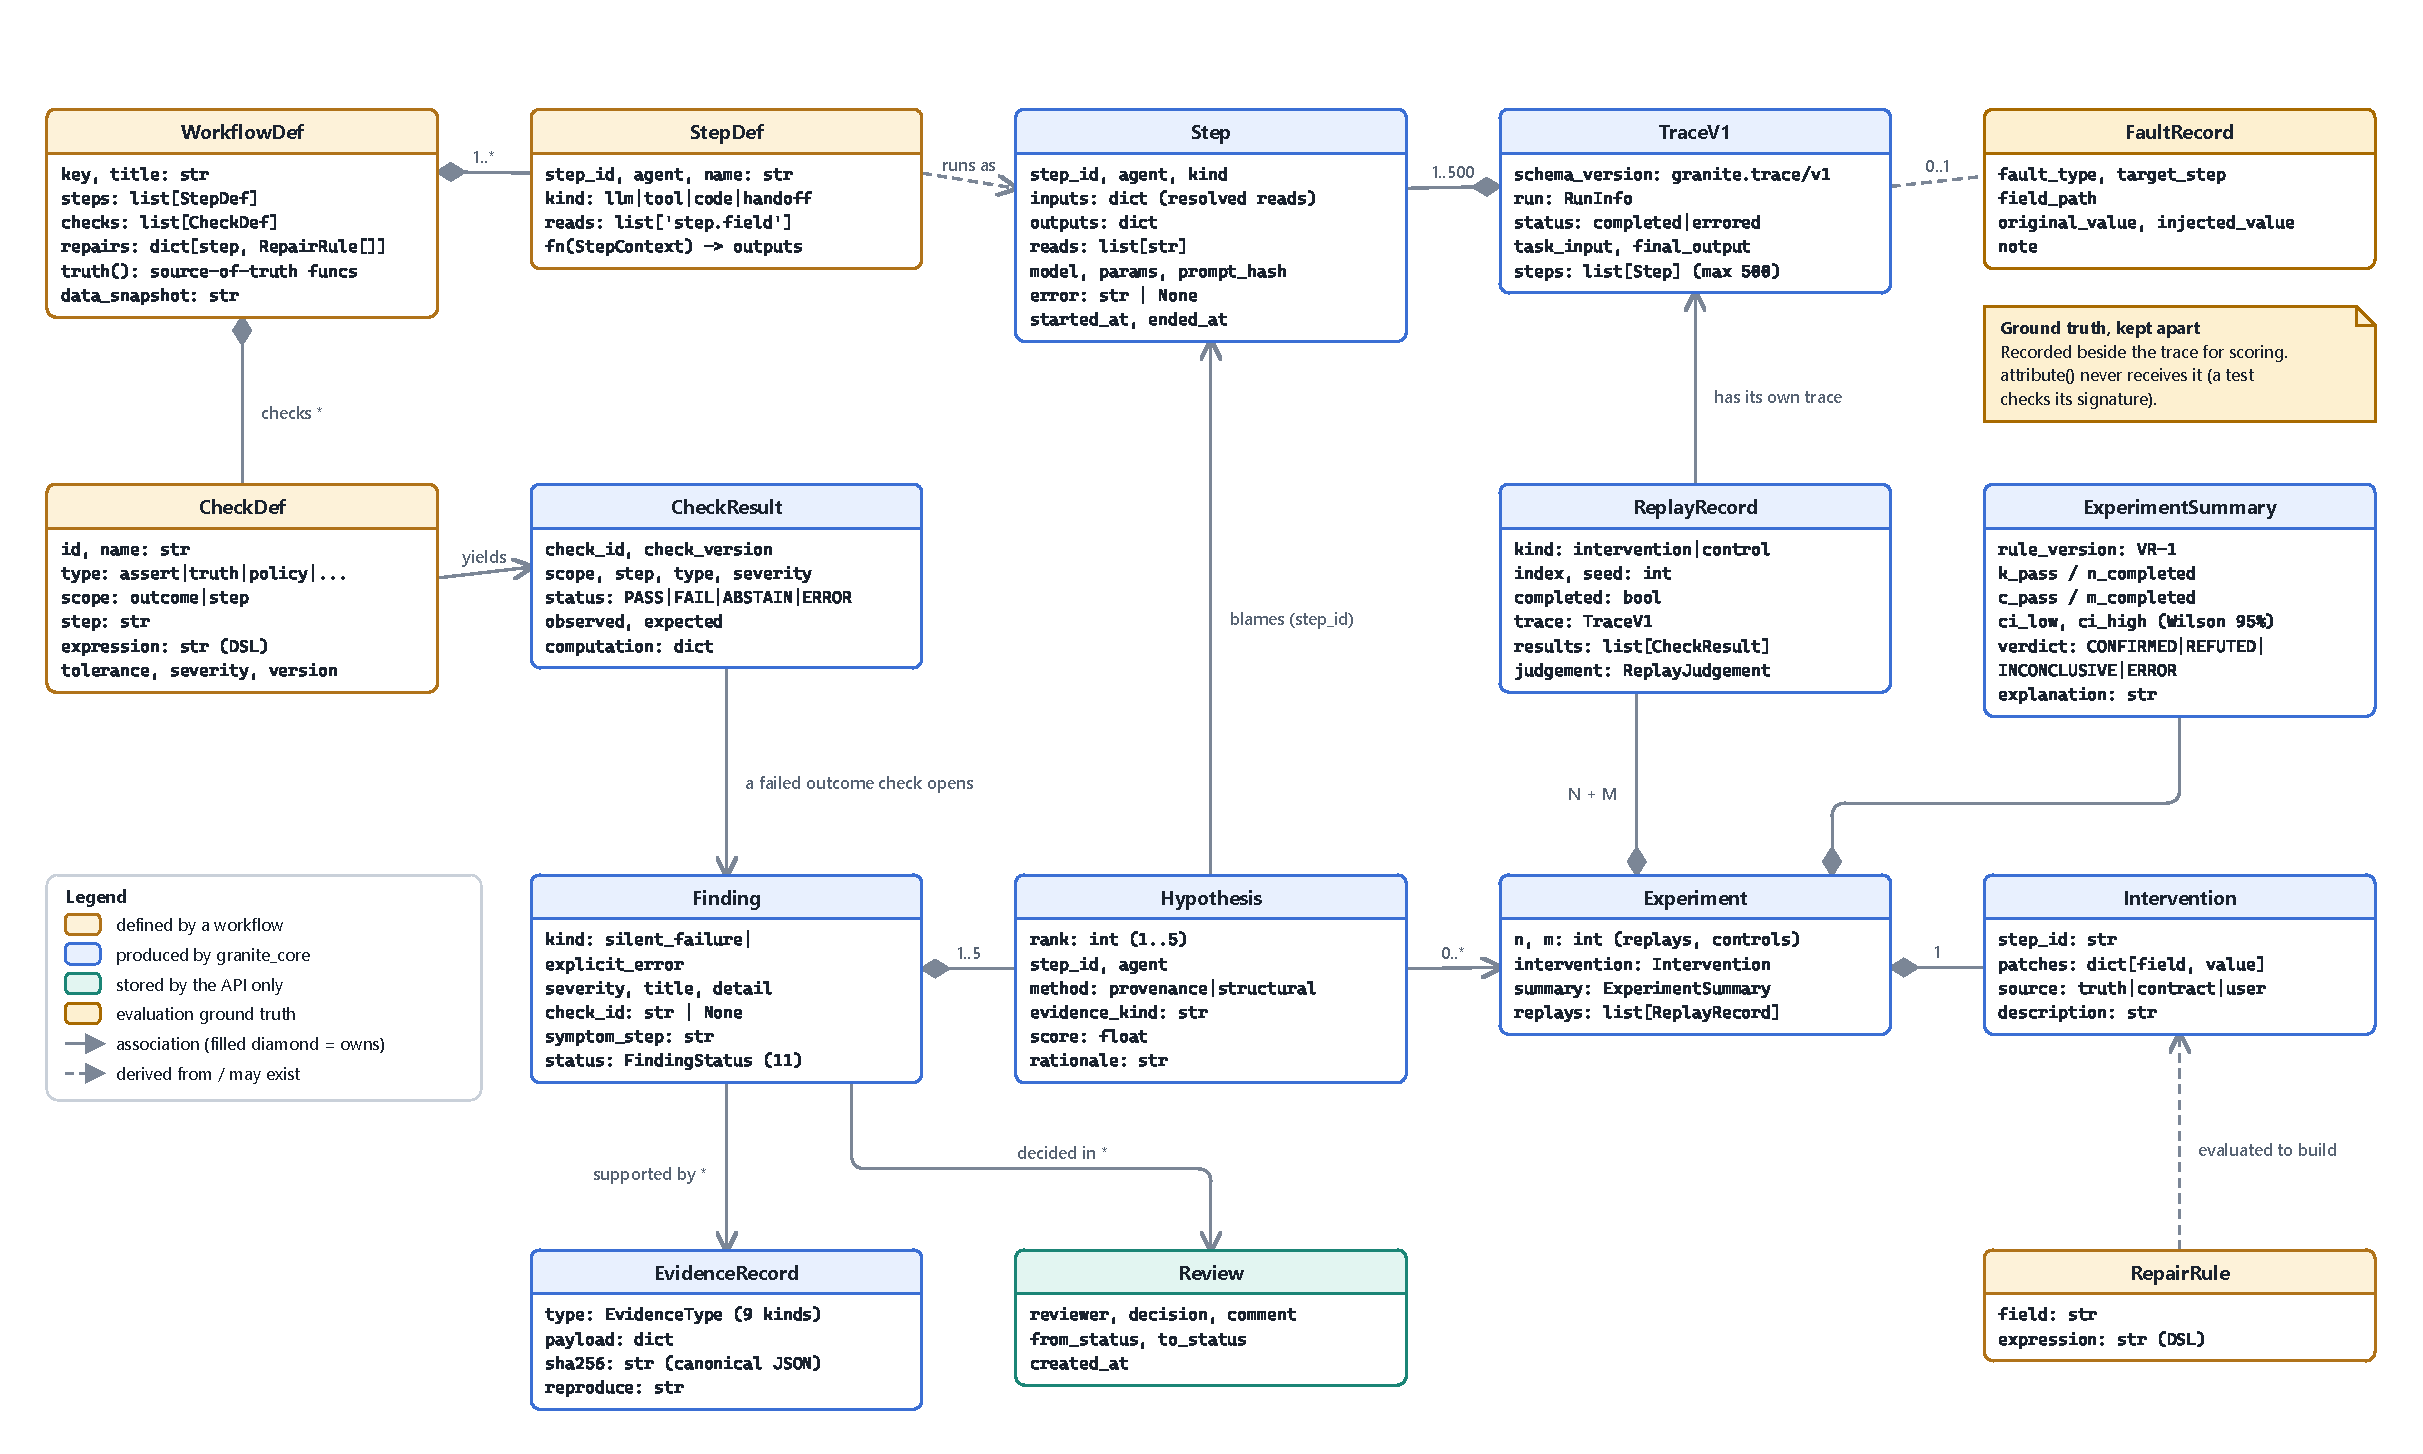
\includegraphics[width=\linewidth,height=0.42\textheight,keepaspectratio]{domain-model.pdf}
\caption{Domain model (class diagram) generated from the code}
\label{fig:domain-model}
\end{figure}


\section{Data Design}

The database has twelve tables, generated into a data dictionary (120 columns) from the models. \texttt{projects} and \texttt{runs} hold the workflow and each execution, with the trace stored as one JSON document and its SHA-256 hash. \texttt{check\_\allowbreak{}results} holds each check's status with observed and expected values. \texttt{fault\_\allowbreak{}injections} holds the ground truth of an injected fault. \texttt{findings} holds each detected failure, its severity, symptom step and lifecycle status. \texttt{hypotheses} holds ranked suspects with method, evidence class and score. \texttt{experiments} and \texttt{replays} hold verification runs and their individual outcomes. \texttt{reviews} holds human decisions. \texttt{evidence} holds typed, hashed, append-only artefacts. \texttt{audit\_\allowbreak{}log} records every state change, and \texttt{jobs} tracks background work. Evidence and audit rows have no update path, so the record cannot be rewritten. The trace itself follows the Granite Trace v1 schema (RunInfo plus a list of Steps).

\begin{figure}[htbp]
\centering
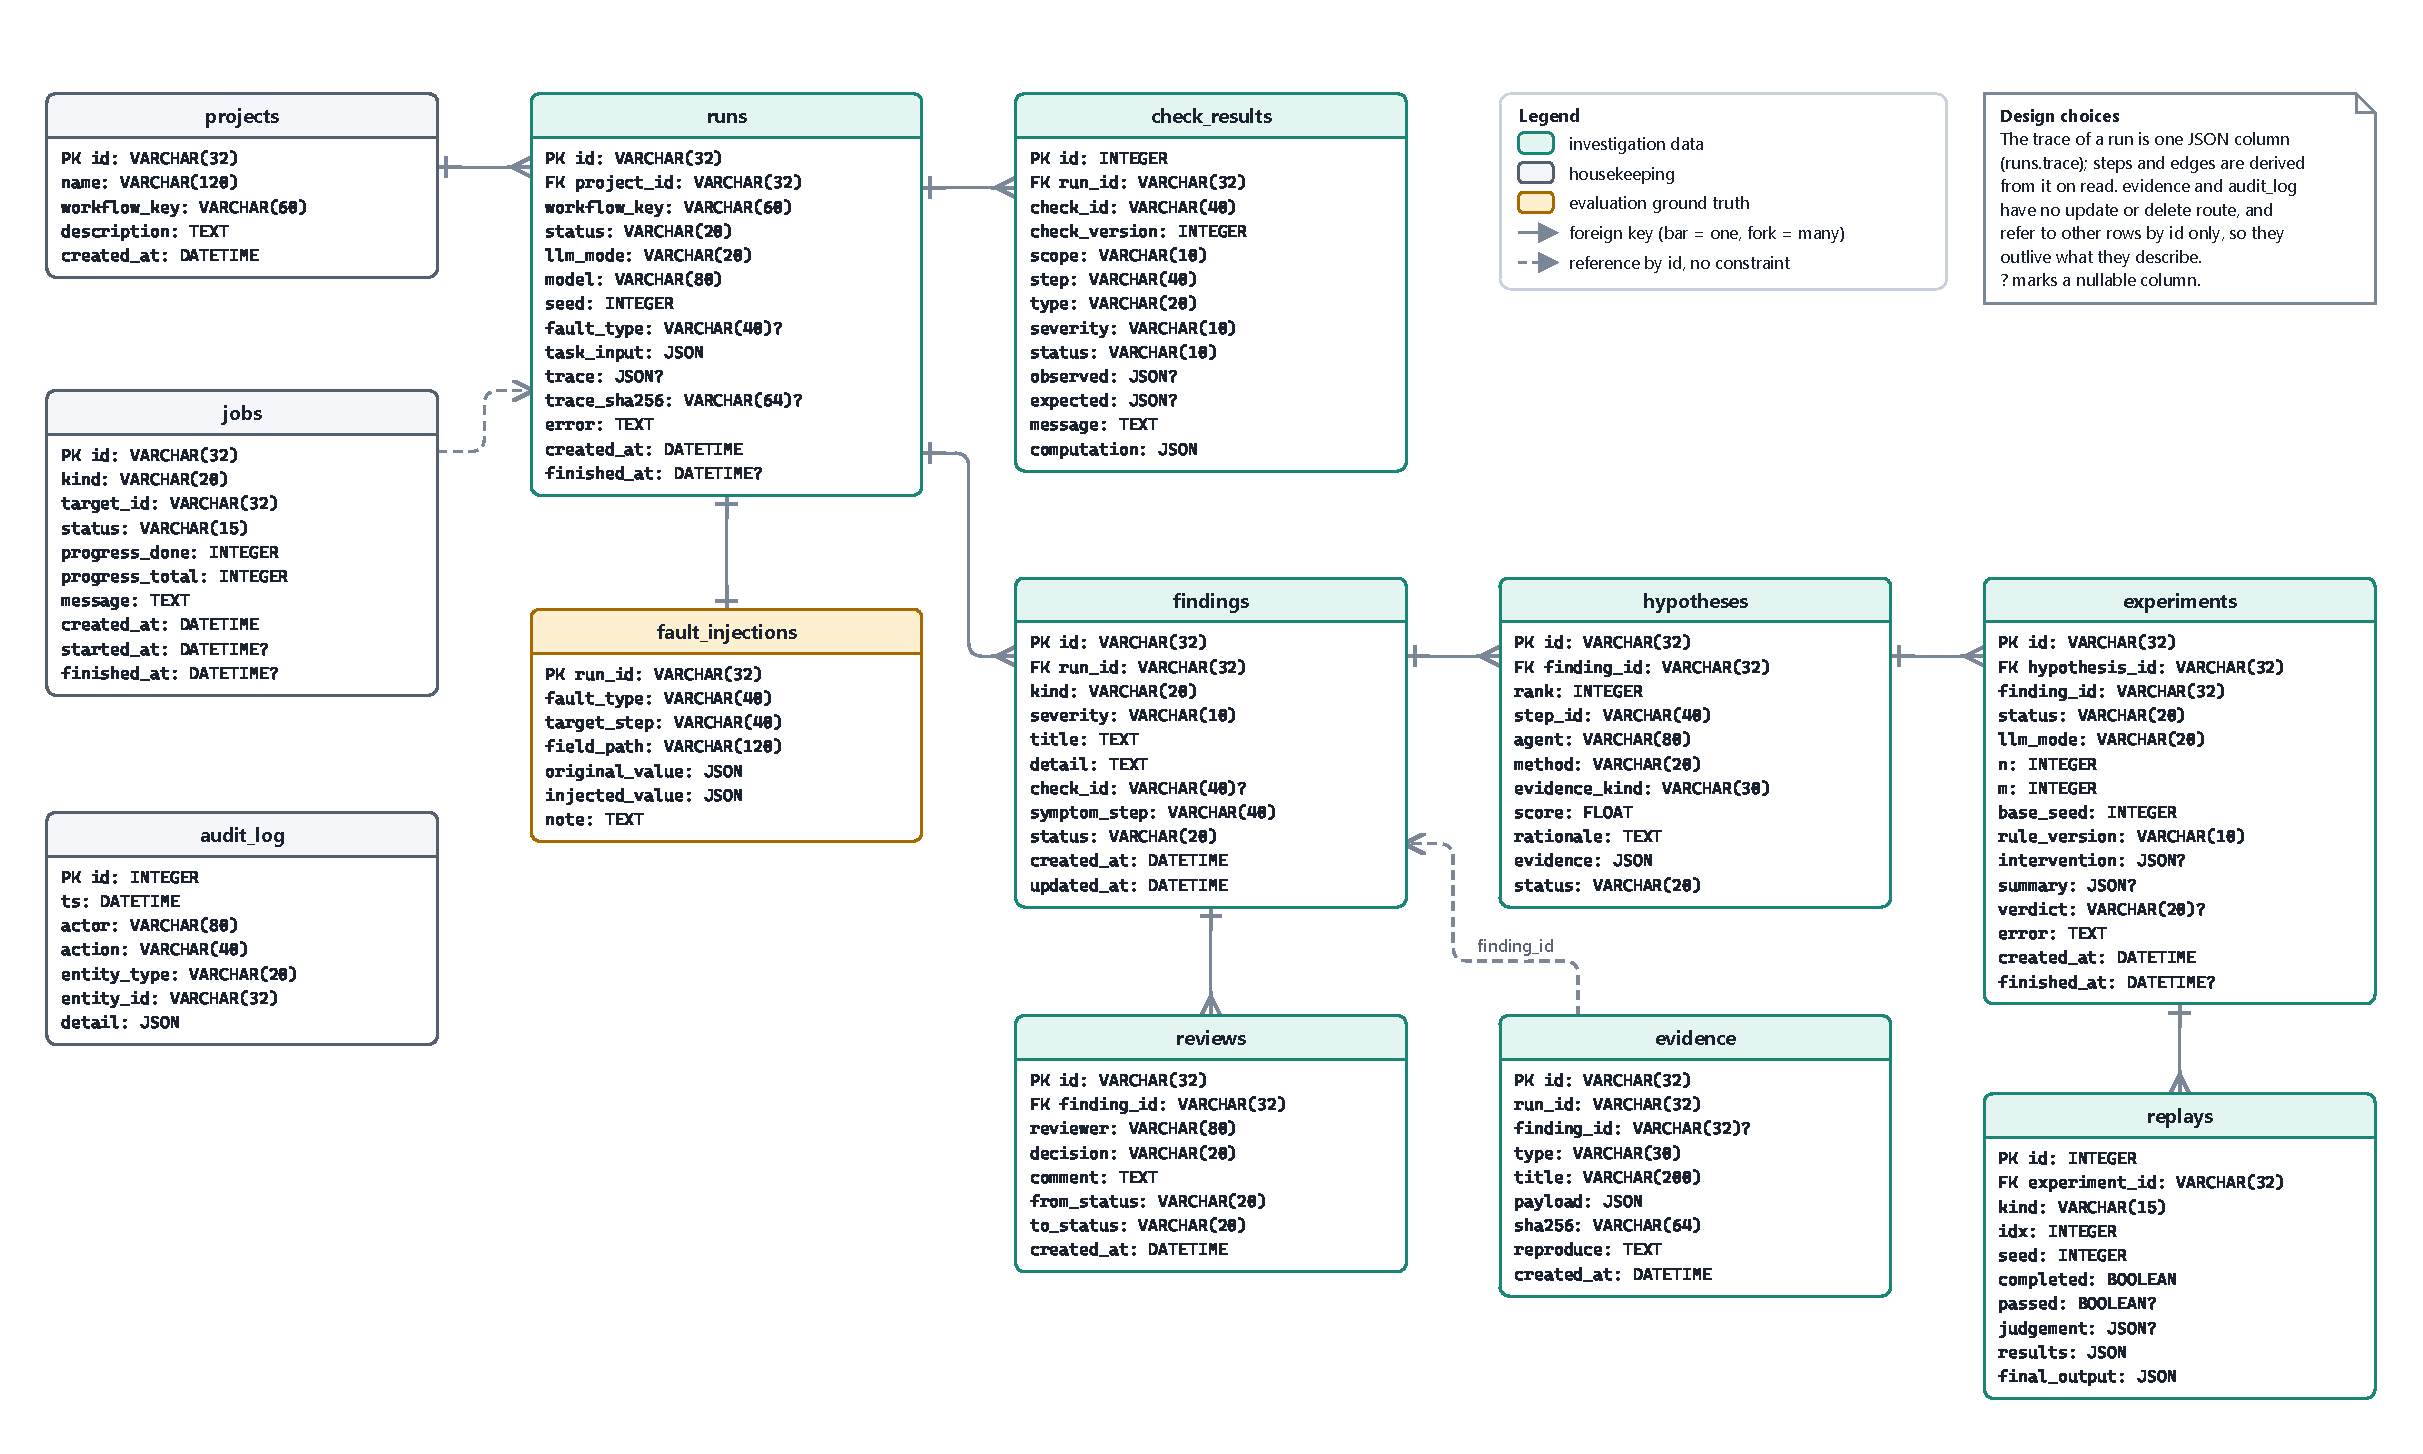
\includegraphics[width=\linewidth,height=0.42\textheight,keepaspectratio]{database-schema.pdf}
\caption{Entity relationship diagram of the twelve tables}
\label{fig:erd}
\end{figure}


\section{Process / Behavior Design}

\textbf{Finding lifecycle.} A finding starts as \textit{open}, becomes \textit{hypothesized} once hypotheses are ranked, and \textit{verifying} when an experiment starts. The verdict moves it to \textit{confirmed}, \textit{refuted} or \textit{inconclusive} (an experiment error returns it to hypothesized). A refuted or inconclusive finding can be verified again (the next hypothesis, or more replays). A confirmed or inconclusive finding is reviewed to \textit{accepted} or \textit{rejected}, and an accepted finding is \textit{resolved} or closed as \textit{won't fix}. Rejected, resolved and won't-fix are terminal. Any other event is refused as an illegal transition. Verification levels follow the state: V0 detected, V1 evidence-reproduced, V2 replay-verified, V3 human-confirmed.

\textbf{Verification sequence.} When the user presses Verify, the API checks that a repair rule exists and stores a queued experiment; a background job builds the intervention (the corrected value), plans the replay (which steps keep their recorded outputs and which re-run), runs N replays with the correction and M without, judges each replay against the target checks, applies VR-1, stores the verdict and replay outputs as evidence, and moves the finding.

\textbf{Data flow.} At level 0, the Developer and Reviewer send tasks, verification requests and decisions to Granite, which exchanges prompts and answers with the LLM Provider and returns runs, findings, verdicts and reports. At level 1, the processes are run workflow, evaluate checks, attribute, verify and review, connected to the stores of the ER diagram.

Figure~\ref{fig:state-machine} shows the lifecycle, Figure~\ref{fig:activity} the activity flow across the five actors, and Figures~\ref{fig:dfd0} and~\ref{fig:dfd1} the data flow at levels 0 and 1.

\begin{figure}[htbp]
\centering
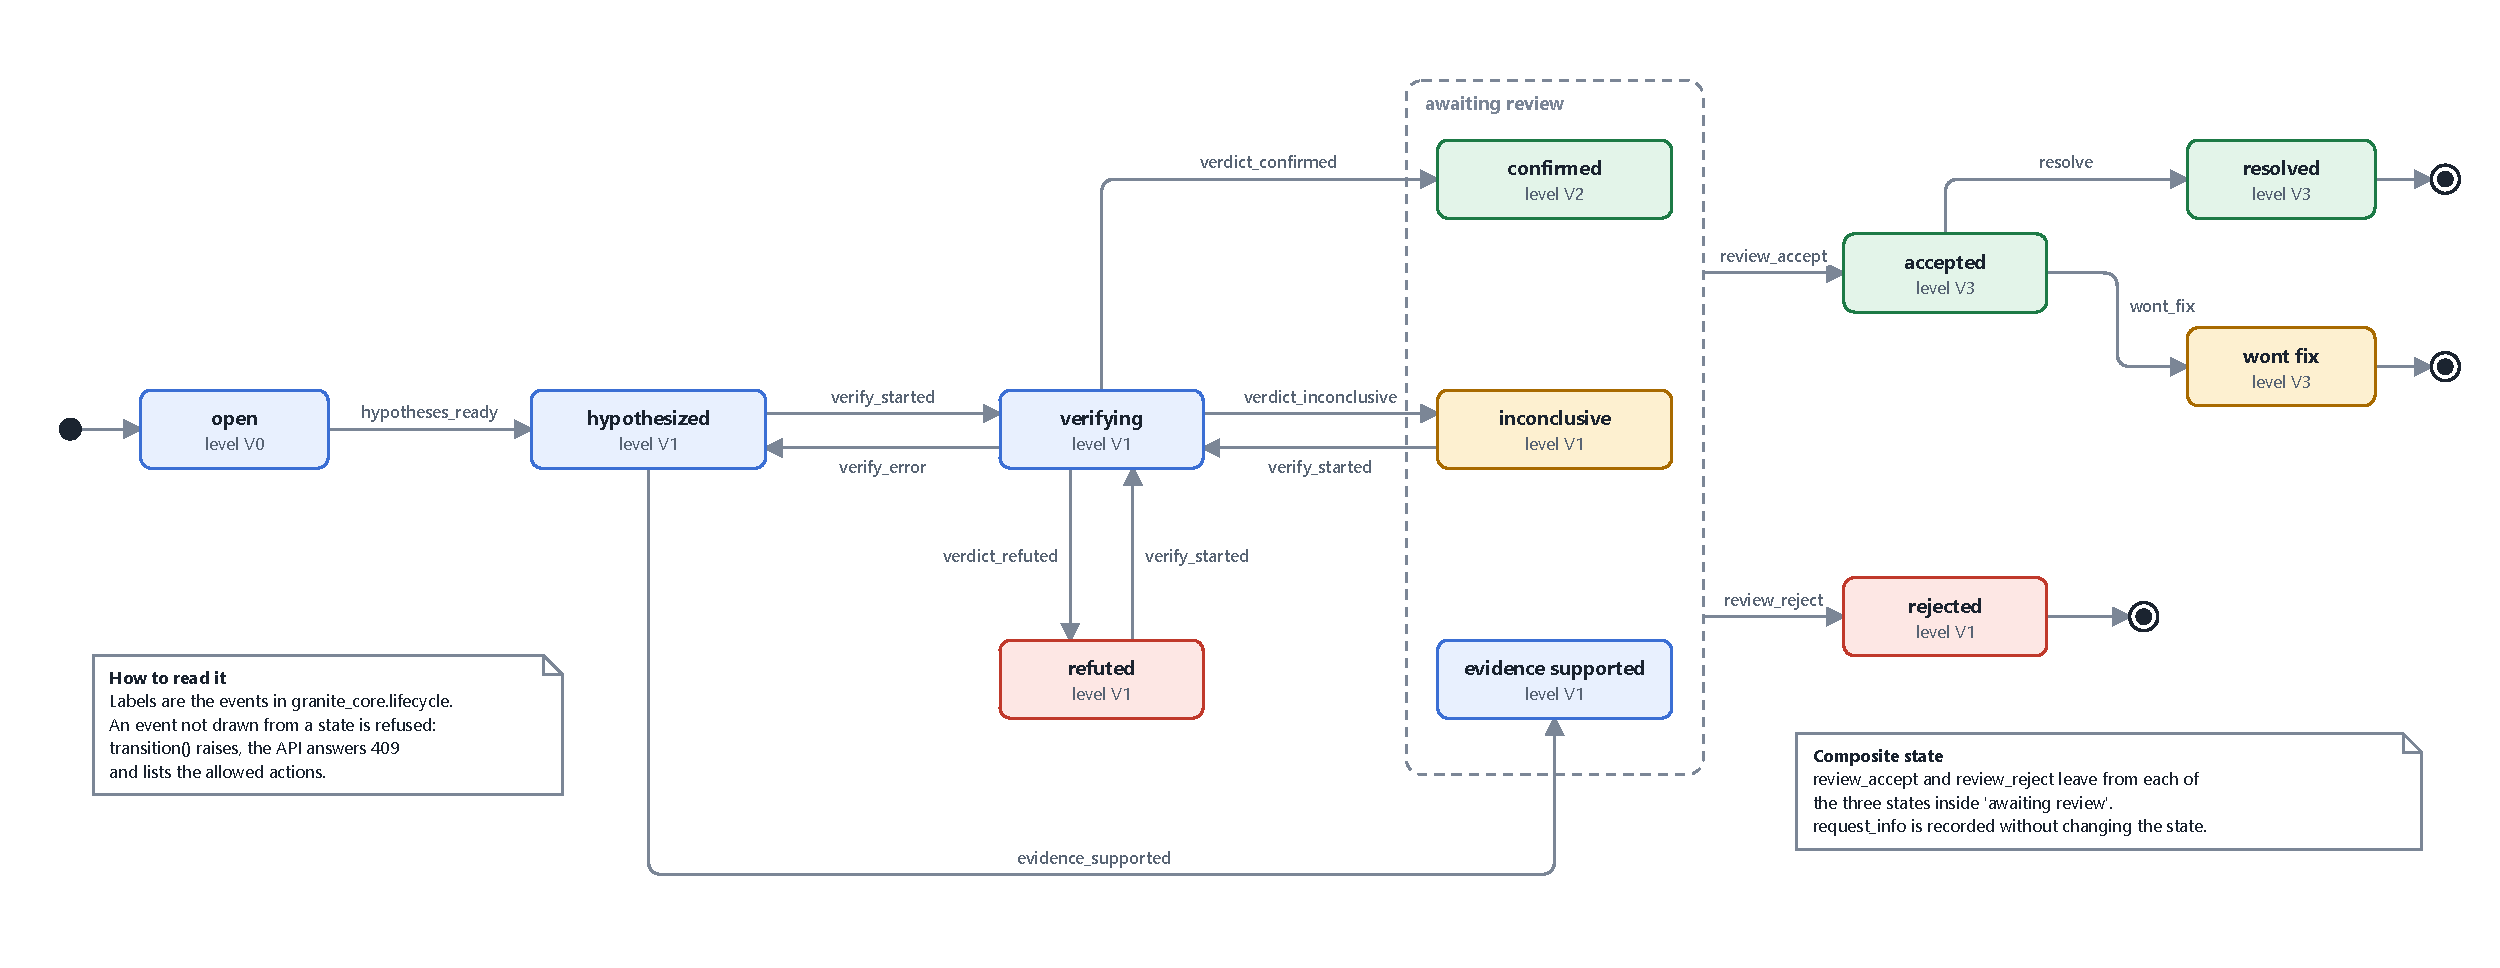
\includegraphics[width=\linewidth,height=0.42\textheight,keepaspectratio]{finding-state-machine.pdf}
\caption{Finding state machine, read from the lifecycle code}
\label{fig:state-machine}
\end{figure}


\begin{figure}[htbp]
\centering
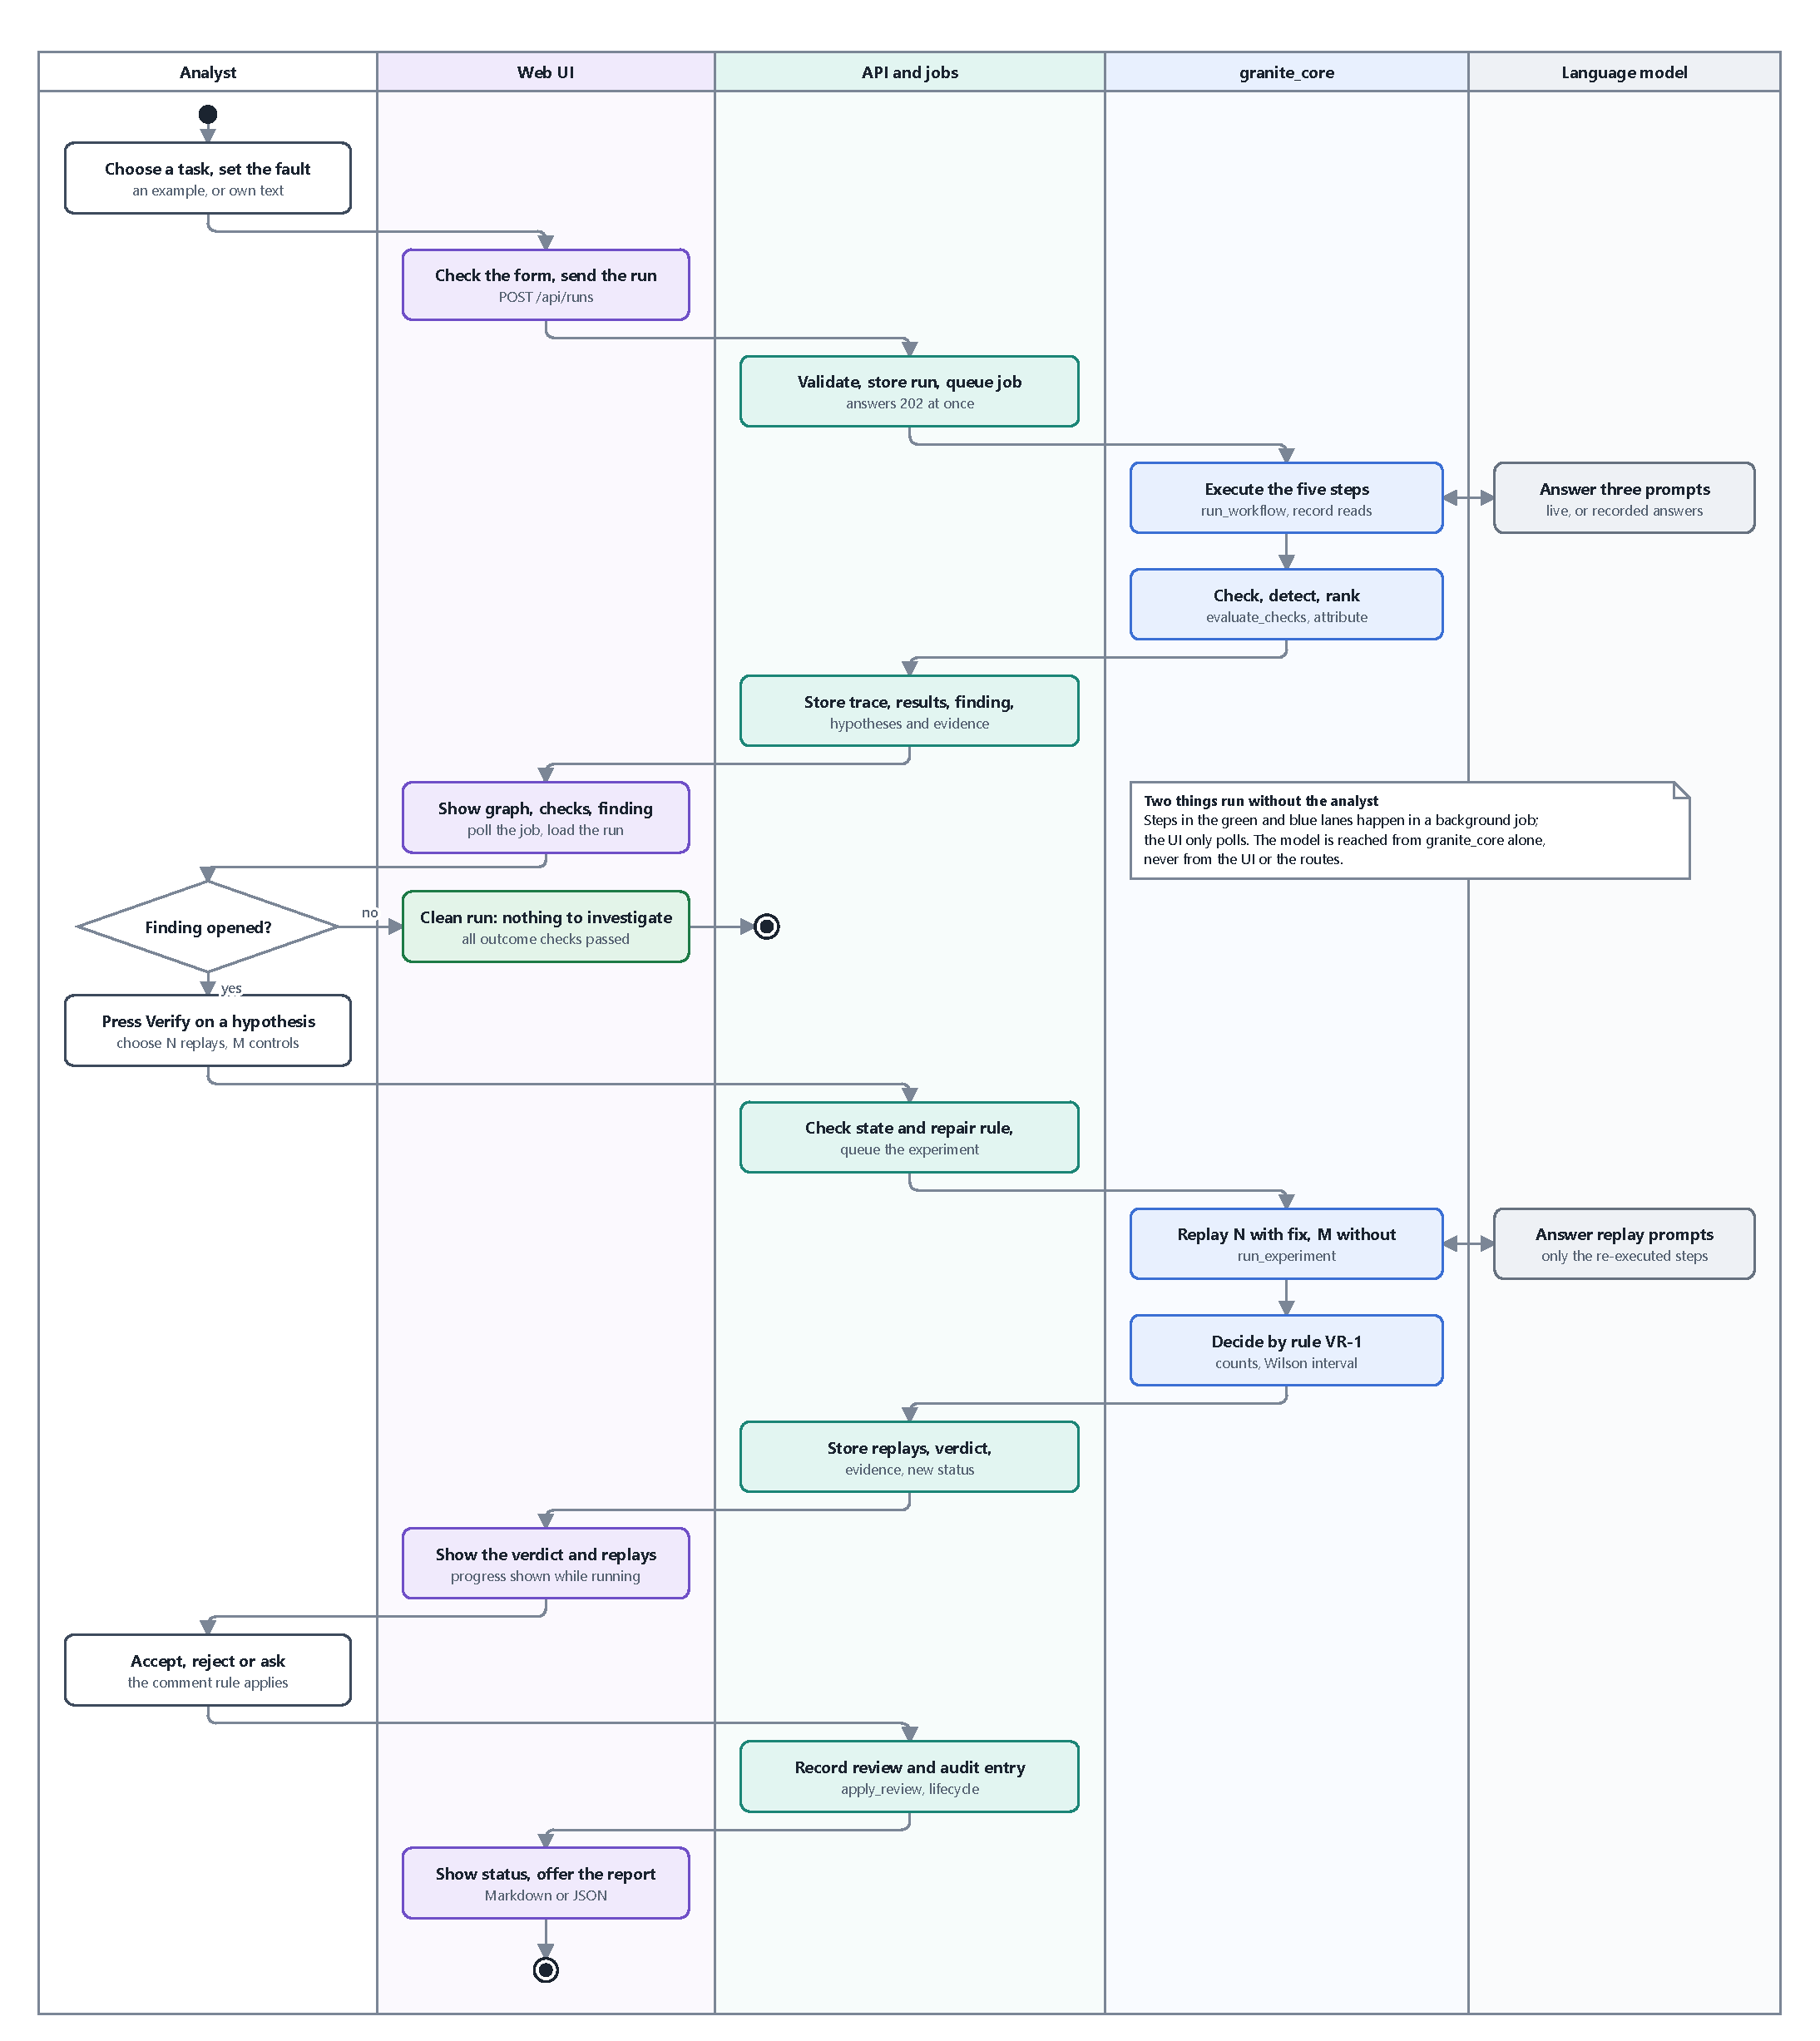
\includegraphics[width=\linewidth,height=0.62\textheight,keepaspectratio]{activity-investigation.pdf}
\caption{Activity diagram of an investigation}
\label{fig:activity}
\end{figure}


\begin{figure}[htbp]
\centering
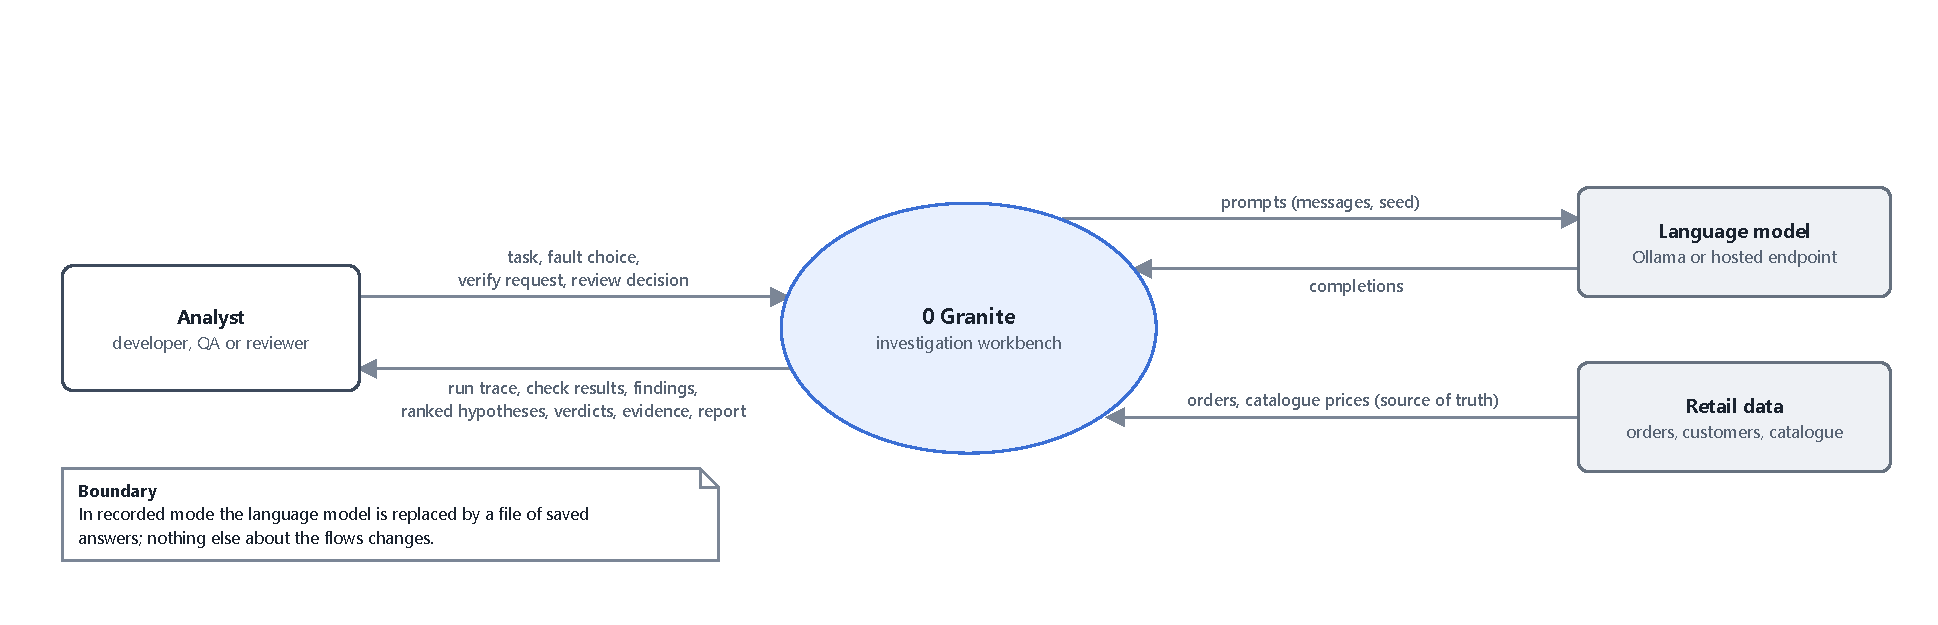
\includegraphics[width=\linewidth,height=0.42\textheight,keepaspectratio]{dfd-context.pdf}
\caption{Data flow diagram, level 0 (context)}
\label{fig:dfd0}
\end{figure}


\begin{figure}[htbp]
\centering
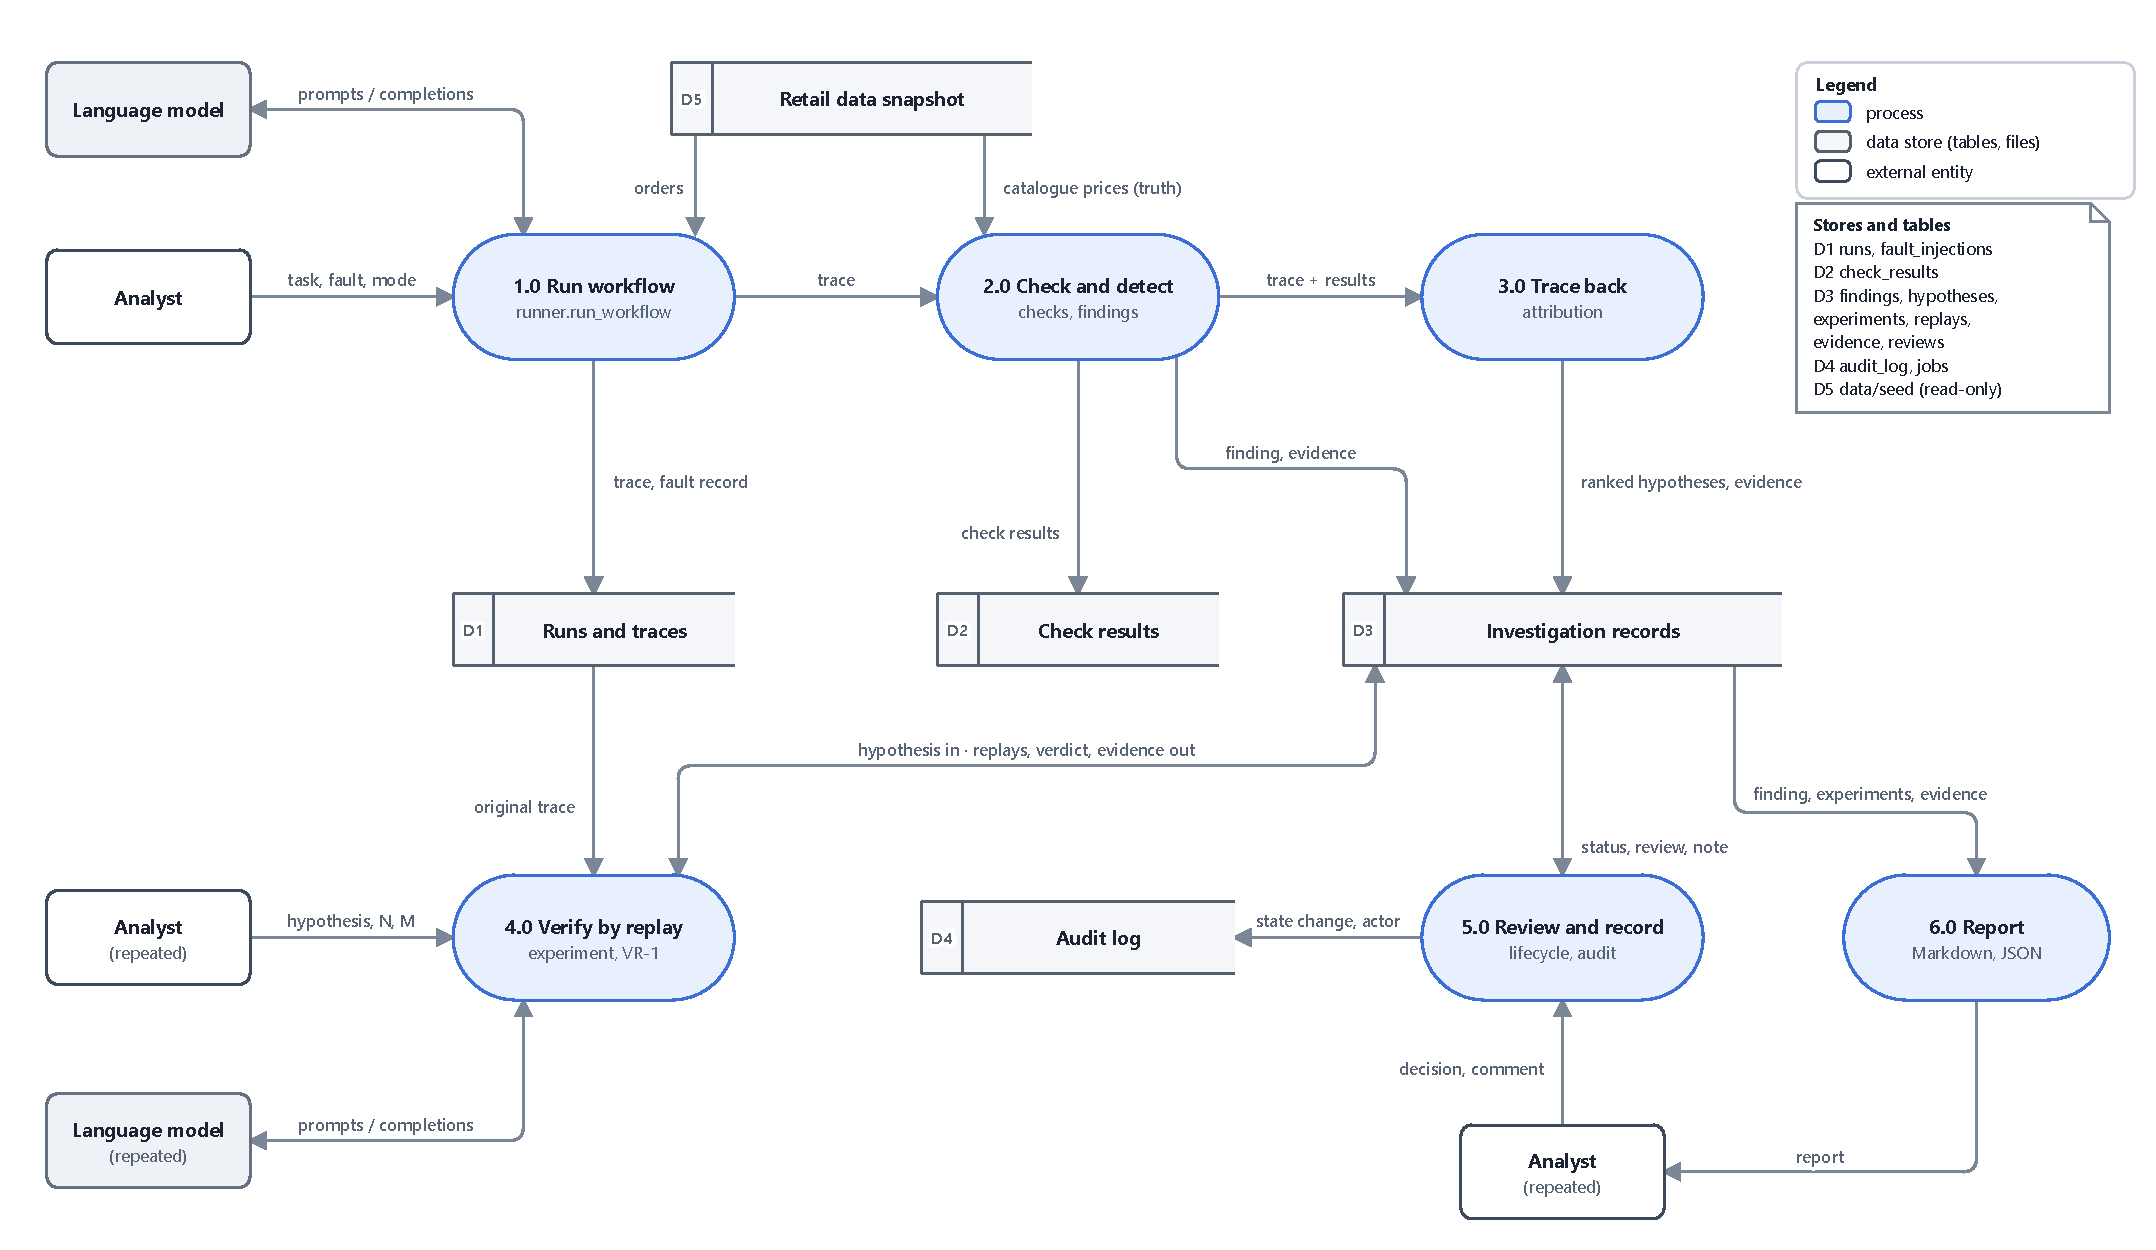
\includegraphics[width=\linewidth,height=0.42\textheight,keepaspectratio]{dfd-level-1.pdf}
\caption{Data flow diagram, level 1}
\label{fig:dfd1}
\end{figure}

%======================================================================================
% chapter6_iteration1
%======================================================================================
\chapter{Iteration 1: Design and Implementation}

This chapter describes the first iteration: its objectives and selected use cases, the design of the Refund Desk workflow used as the system under test, how the implementation is organised, the algorithms at its core, the tools used, and the evidence that the iteration works.

\section{Iteration Objectives}

Build one complete, working investigation slice: run a real multi-agent workflow on real data with a real model, detect a silent failure without an answer key, trace it to its origin, verify the cause with controls, record a human decision, and export the evidence. Deliver it with automated tests, CI, a deployed instance and design artefacts that match the code.

\section{Selected Use Cases / Features}

UC-03 (run), UC-05 (inspect), UC-06 (analyse), UC-07 (investigate), UC-08 (verify), UC-09 (review), UC-12 (history) and the report part of UC-11. These became eight features: F1 Run, F2 Check and detect, F3 Trace back, F4 Verify, F5 Review, F6 Evidence and report, F7 Find, F8 Guide.

\section{Design}

The Refund Desk has five steps, each declaring what it reads: s1 Intake (LLM) extracts the order number and items from the message; s2 Order Lookup (tool) fetches the order and prices from the store; s3 Policy (deterministic code) decides eligibility from the order status, owner and items; s4 Refund Calculator (LLM) adds up the refund; s5 Writer (LLM) writes the reply. Seven checks are attached: two outcome checks (the stated refund equals the catalogue total of the refunded items; the decision follows policy) and five step contracts, one per step. Repair rules say how to compute the correct output of a step, which verification uses as its intervention. The stale-price fault lowers one requested item's price by \$0.25 at s2 without raising an error. (Figure~\ref{fig:refund-dataflow})

\section{Implementation}

{\small
\begin{longtable}{>{\raggedright\arraybackslash\hspace{0pt}}p{0.181\linewidth}>{\raggedright\arraybackslash\hspace{0pt}}p{0.053\linewidth}>{\raggedright\arraybackslash\hspace{0pt}}p{0.058\linewidth}>{\raggedright\arraybackslash\hspace{0pt}}p{0.568\linewidth}}
\caption{Implementation}\label{tab:chapter6_iteration1-1}\\
\toprule
\textbf{Package} & \textbf{Files} & \textbf{Tests} & \textbf{Responsibility} \\
\midrule
\endfirsthead
\toprule
\textbf{Package} & \textbf{Files} & \textbf{Tests} & \textbf{Responsibility} \\
\midrule
\endhead
\bottomrule
\endlastfoot
\texttt{packages/\allowbreak{}granite\_\allowbreak{}core} & 13 & 207 & Trace, runner, check language, checks, lineage, attribution, verification, experiment, lifecycle, evidence, LLM provider interfaces, redaction \\
\texttt{workflows/\allowbreak{}refund\_\allowbreak{}desk} & 5 & 49 & Steps, checks, repair rules, fault, retail store \\
\texttt{apps/\allowbreak{}api} & 20 & 71 & Endpoints, schemas, models, services, jobs, providers, errors \\
\texttt{apps/\allowbreak{}web} & 16 & 32 & Five screens and shared components \\
\texttt{tests/\allowbreak{}system} & --- & 22 & Black-box tests over HTTP \\
\end{longtable}
}

A run request flows as follows: the New run page posts the task; the route checks the token and rate limit and returns 202 with a job; the run service validates the task, stores a queued run and starts a job; the runner executes the five steps and records the trace, applying the fault if requested; the analysis service stores the trace and hash, evaluates the checks, opens findings, ranks hypotheses and writes evidence. A verification request flows through the experiment service, \texttt{build\_\allowbreak{}intervention} and \texttt{plan\_\allowbreak{}replay}, \texttt{run\_\allowbreak{}experiment} (N + M replays with their own seeds), \texttt{decide} (VR-1) and \texttt{transition} (lifecycle).

Figure~\ref{fig:structure-chart} shows the modules and functions involved.

\begin{figure}[htbp]
\centering
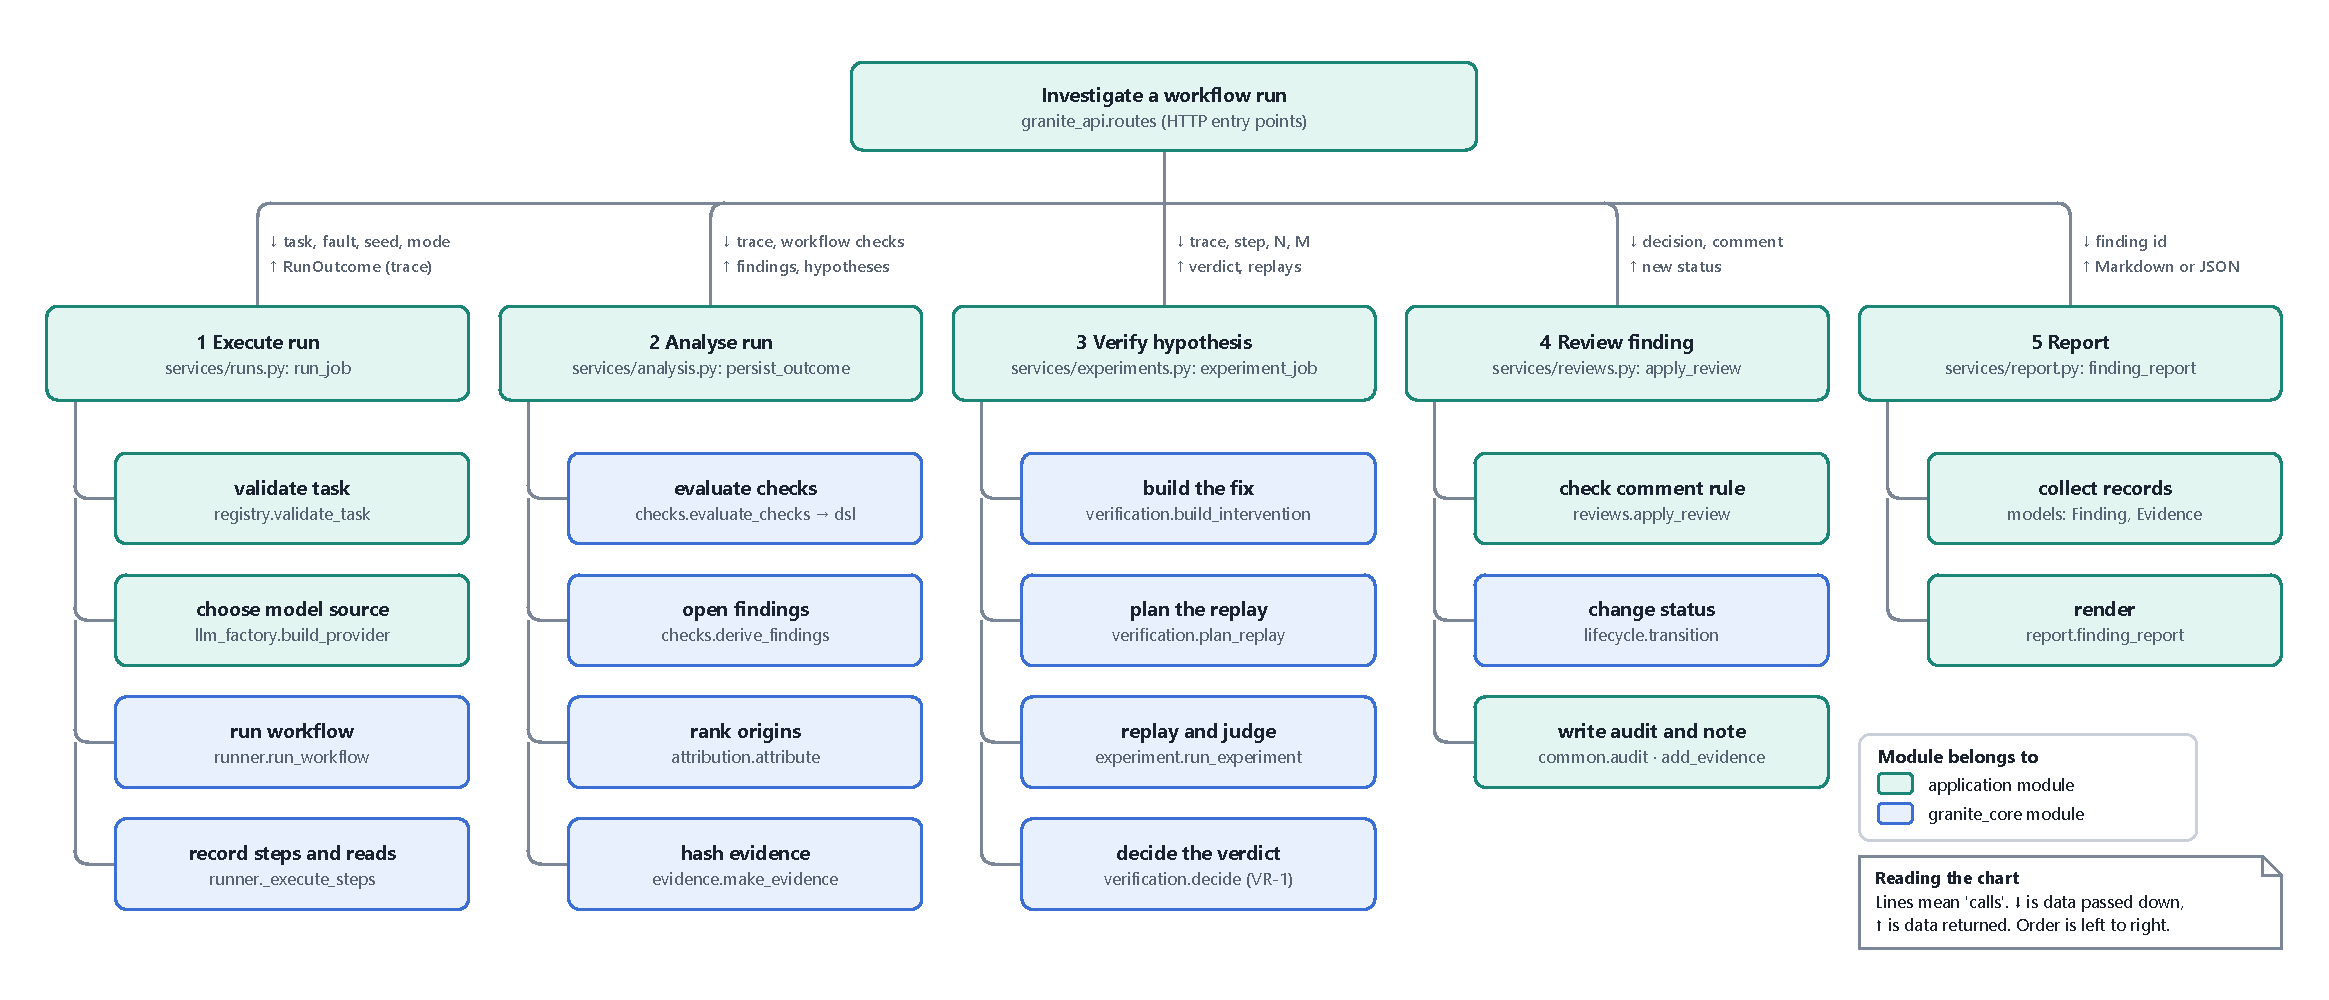
\includegraphics[width=\linewidth,height=0.42\textheight,keepaspectratio]{structure-chart.pdf}
\caption{Structure chart with the real function names}
\label{fig:structure-chart}
\end{figure}


\section{Completed Features / Module}

All eight features are implemented and tested: run and record every step (F1), check the outcome and detect silent failures (F2), trace back to where it began (F3), verify by controlled replay (F4), review (F5), evidence and report export (F6), find earlier runs and findings (F7) and the in-product guide and API reference (F8). Not yet built and not claimed: trace import, a second workflow, a check editor, fix suggestions, PDF export and redaction of stored data.

\section{Technical Implementation Details}

\textbf{Reproducible setup} (from the setup manual; works on Windows, Linux and macOS with Python 3.11 and Node 20+):

\begin{lstlisting}[basicstyle=\ttfamily\footnotesize,breaklines=true,columns=fullflexible]
python -m venv .venv && source .venv/bin/activate        # Windows: .venv\Scripts\activate
pip install -e "packages/granite_core[dev]" -e "workflows/refund_desk[dev]" -e "apps/api[dev]"
(cd apps/web && npm ci && npm run build)
cd apps/api
GRANITE_LLM_MODE=recorded GRANITE_STATIC_DIR=../web/dist uvicorn granite_api.main:app_from_env --factory --port 8000
\end{lstlisting}

Open \url{http://127.0.0.1:8000}. Recorded mode needs no model or key. For live mode, install Ollama, run \texttt{ollama pull llama3.\allowbreak{}2:3b}, and set \texttt{GRANITE\_\allowbreak{}LLM\_\allowbreak{}MODE=live}. The container runs with \texttt{docker compose up}. The setup was repeated on a second team member's laptop on 11 October and all 381 tests passed.

\textbf{Key technical details:} each step's inputs are resolved from its declared reads, so the data flow is recorded rather than inferred. Traces are stored as canonical JSON and hashed with SHA-256. Recorded answers are keyed by a hash of model, messages, parameters and seed; a missing answer raises an error instead of inventing one. Model outputs are requested as JSON and parsed; invalid JSON fails the step visibly. Background work runs in a thread pool with a job table. Errors follow RFC 7807, and internal exception text never reaches the client.

\section{Algorithms and Technical Decisions}

\textbf{Check language.} A check is an expression such as \texttt{approx(\allowbreak{}number\_\allowbreak{}in(\allowbreak{}s5.\allowbreak{}message),\allowbreak{} truth.\allowbreak{}catalog\_\allowbreak{}total(\allowbreak{}pluck(\allowbreak{}s3.\allowbreak{}items\_\allowbreak{}to\_\allowbreak{}refund,\allowbreak{} 'item\_\allowbreak{}id')))}. It is parsed with Python's \texttt{ast} module and accepted only if every syntax node and function is on a whitelist, within 500 characters, 150 nodes and depth 14; it is then evaluated by our own interpreter, never by \texttt{eval}. A missing field gives ABSTAIN, not PASS.

\textbf{Attribution.} Starting from the symptom step, the algorithm walks backwards along the lineage edges that carry the failing field and classifies each step by its evidence: truth mismatch (weight 1.0), contract failure (0.8), hand-off drift where a step's input differs from what upstream produced (0.7), no check defined (0.2) or consistent (0). Candidates are ranked by weight, then by earliest position, with a decay for distance from the symptom. If no step has direct evidence (weight $\geq$ 0.7), all candidates are labelled "structural only, needs verification." Complexity is O(V + E). No language model is used.

\textbf{Verdict rule VR-1.} With k of N intervention replays passing (p = k/N) and c of M controls passing (q = c/M): CONFIRMED if p $\geq$ 0.8 and q $\leq$ 0.2; REFUTED if p $\leq$ 0.2; otherwise INCONCLUSIVE; ERROR if fewer than N replays complete. A 95\% Wilson interval is reported but not used to decide at N = 5. A replay that causes a new check failure counts as not passing (regression guard). Thresholds are versioned; a change would create VR-2.

\textbf{Replay plan.} To test a hypothesis about step s, outputs of all steps before s are kept from the original trace, s's output is replaced with the corrected value from its repair rule, and only the steps after s are re-executed, so frozen steps cost no model calls.

Figures~\ref{fig:check-pipeline} to~\ref{fig:replay-plan} show the four algorithms.

\begin{figure}[htbp]
\centering
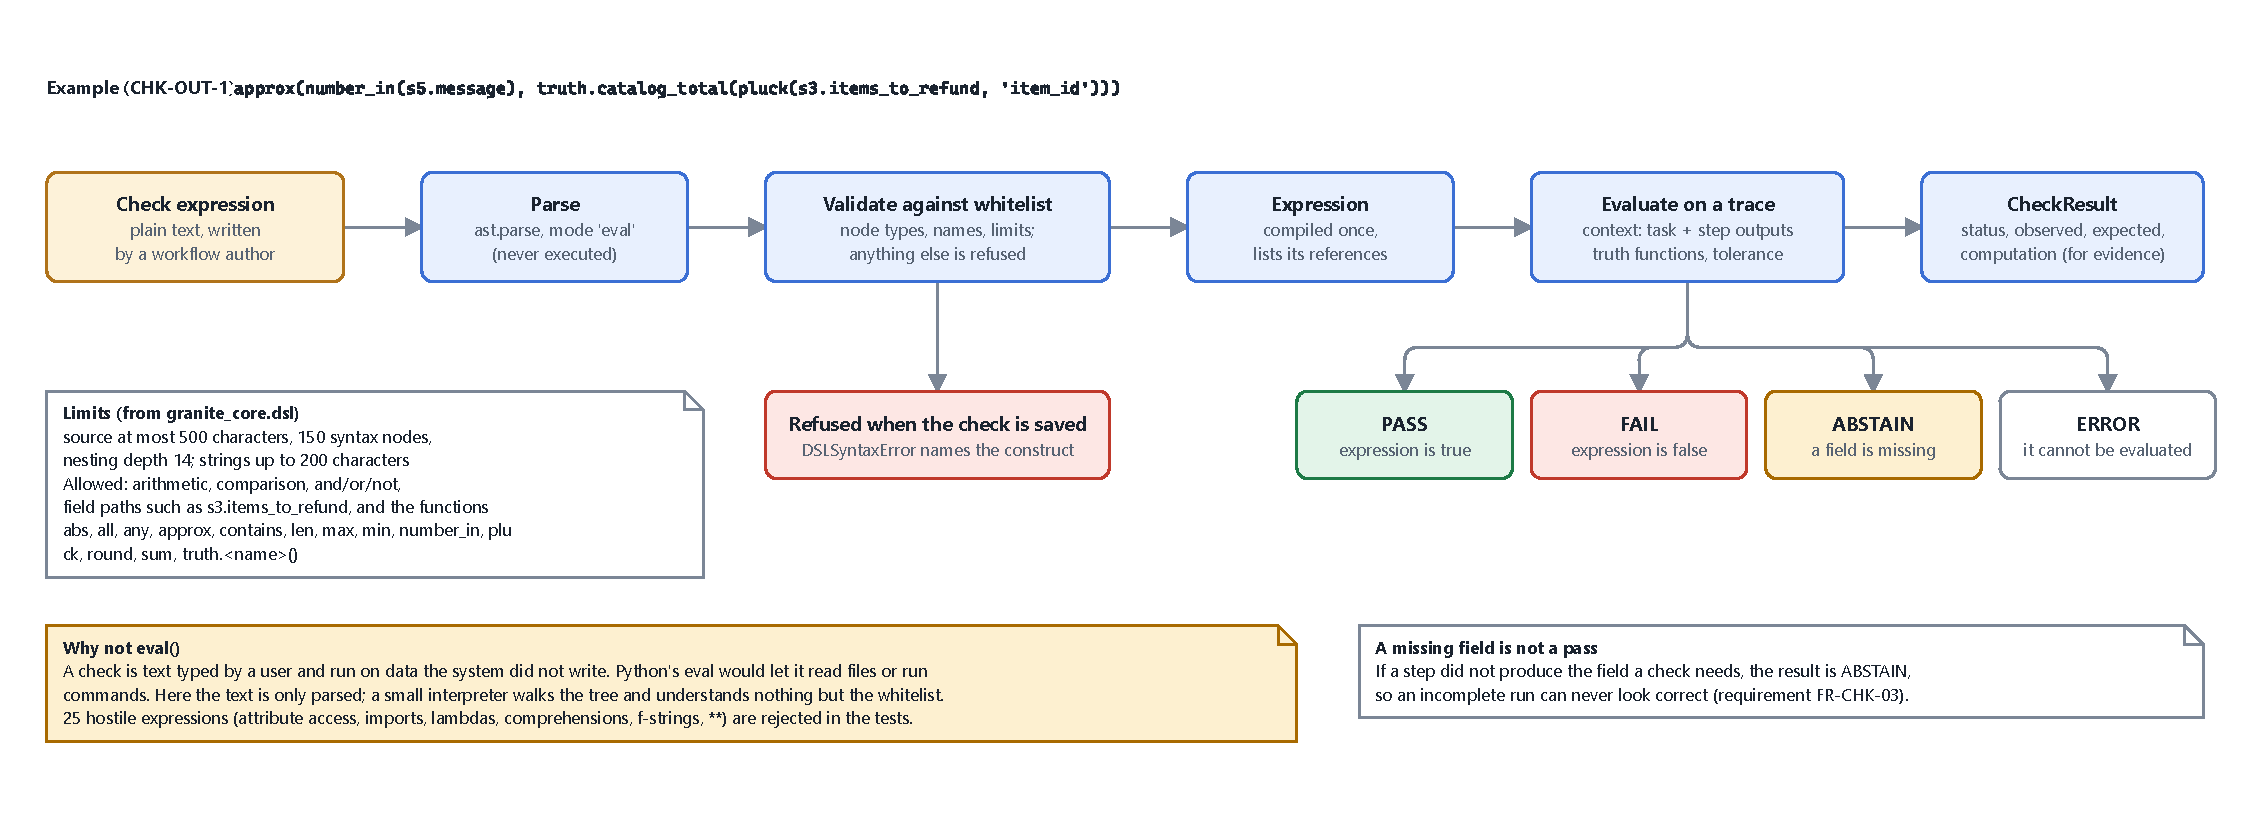
\includegraphics[width=\linewidth,height=0.42\textheight,keepaspectratio]{check-pipeline.pdf}
\caption{Check language: from expression text to result}
\label{fig:check-pipeline}
\end{figure}


\begin{figure}[htbp]
\centering
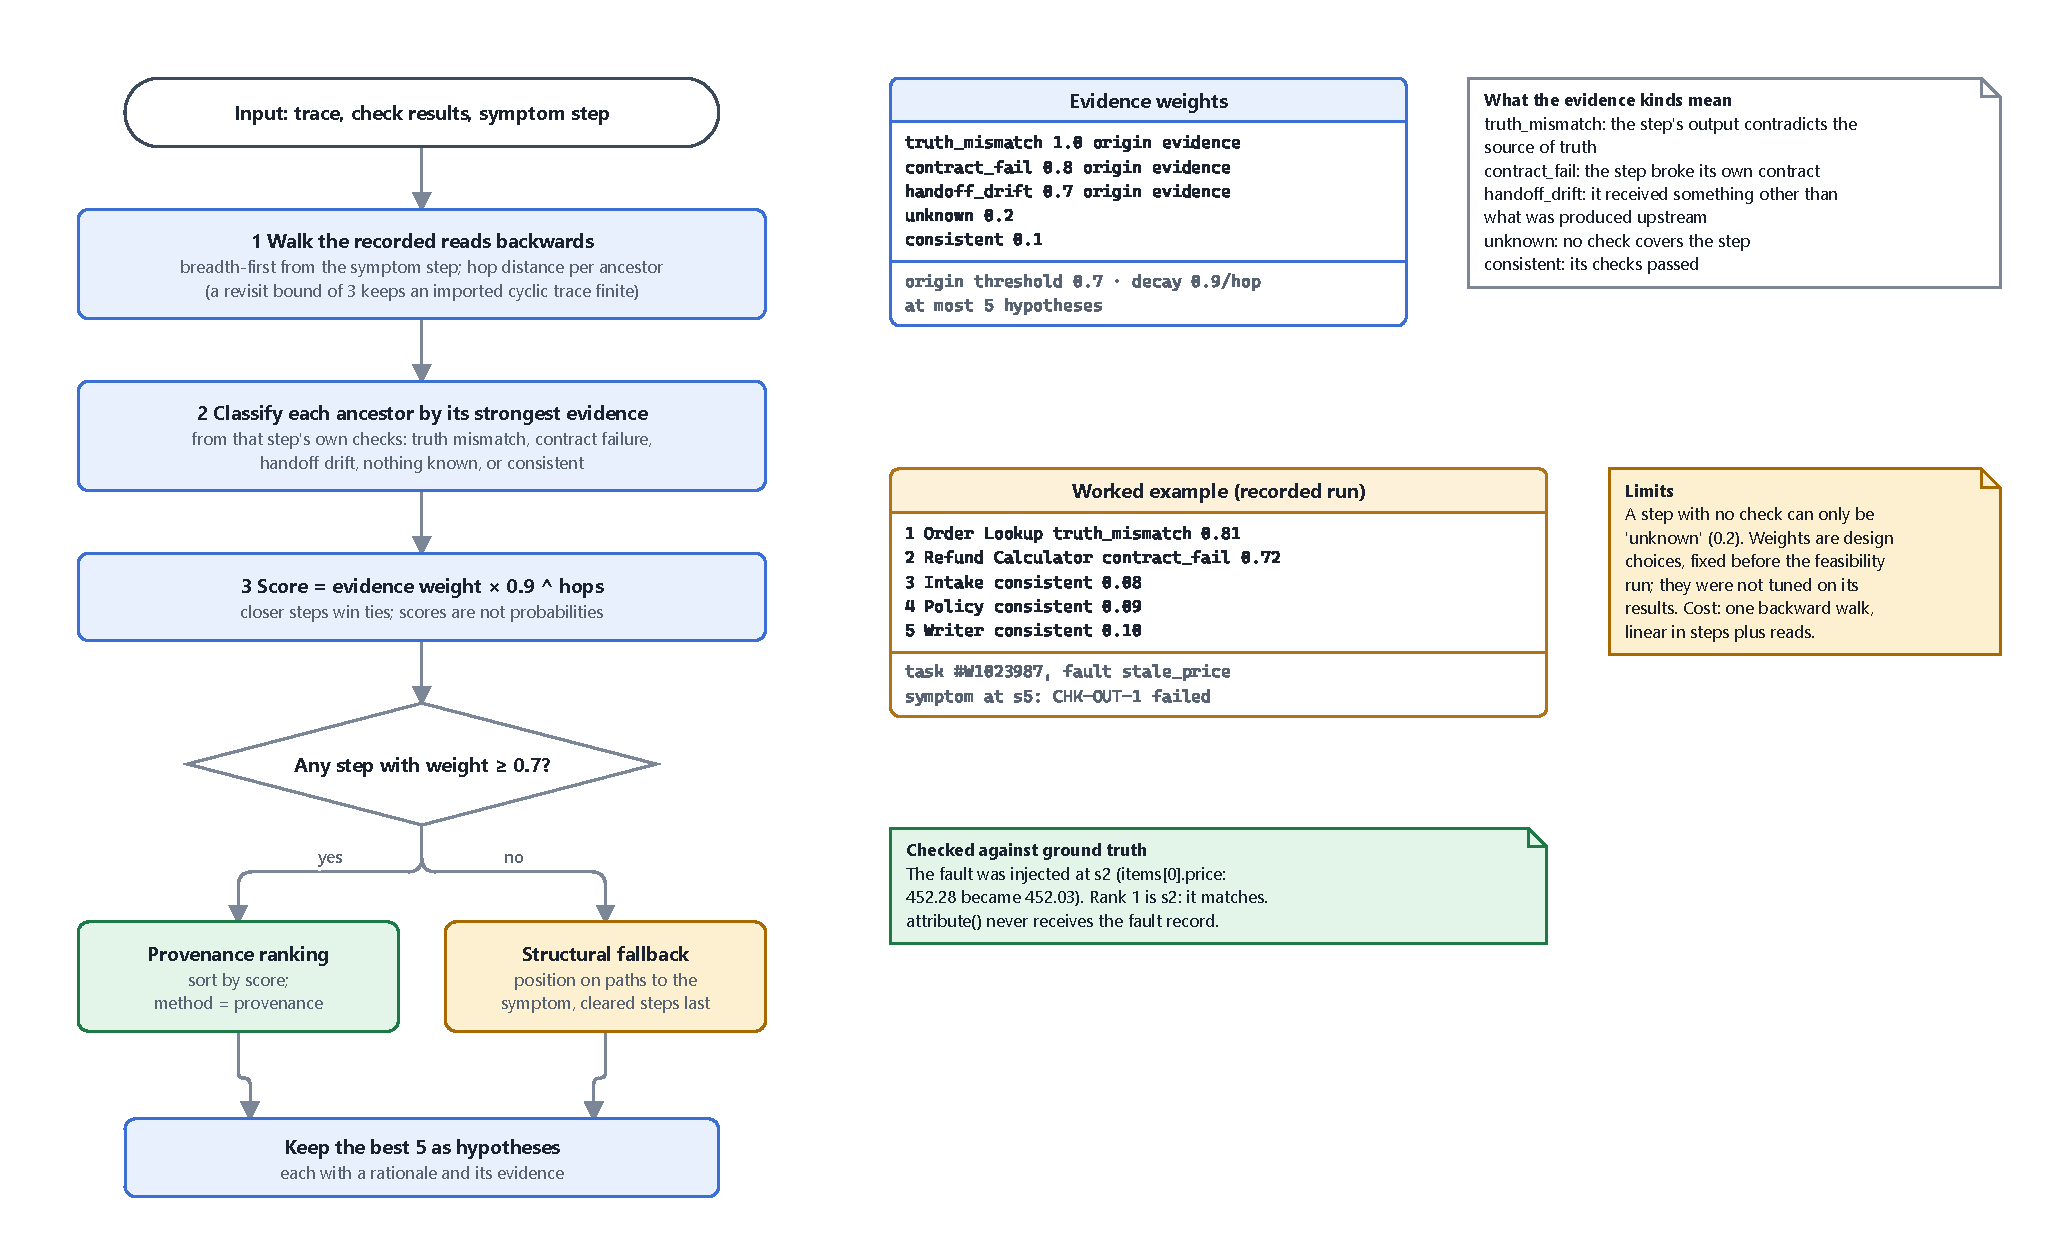
\includegraphics[width=\linewidth,height=0.42\textheight,keepaspectratio]{attribution-algorithm.pdf}
\caption{Attribution: ranking where a failure began}
\label{fig:attribution}
\end{figure}


\begin{figure}[htbp]
\centering
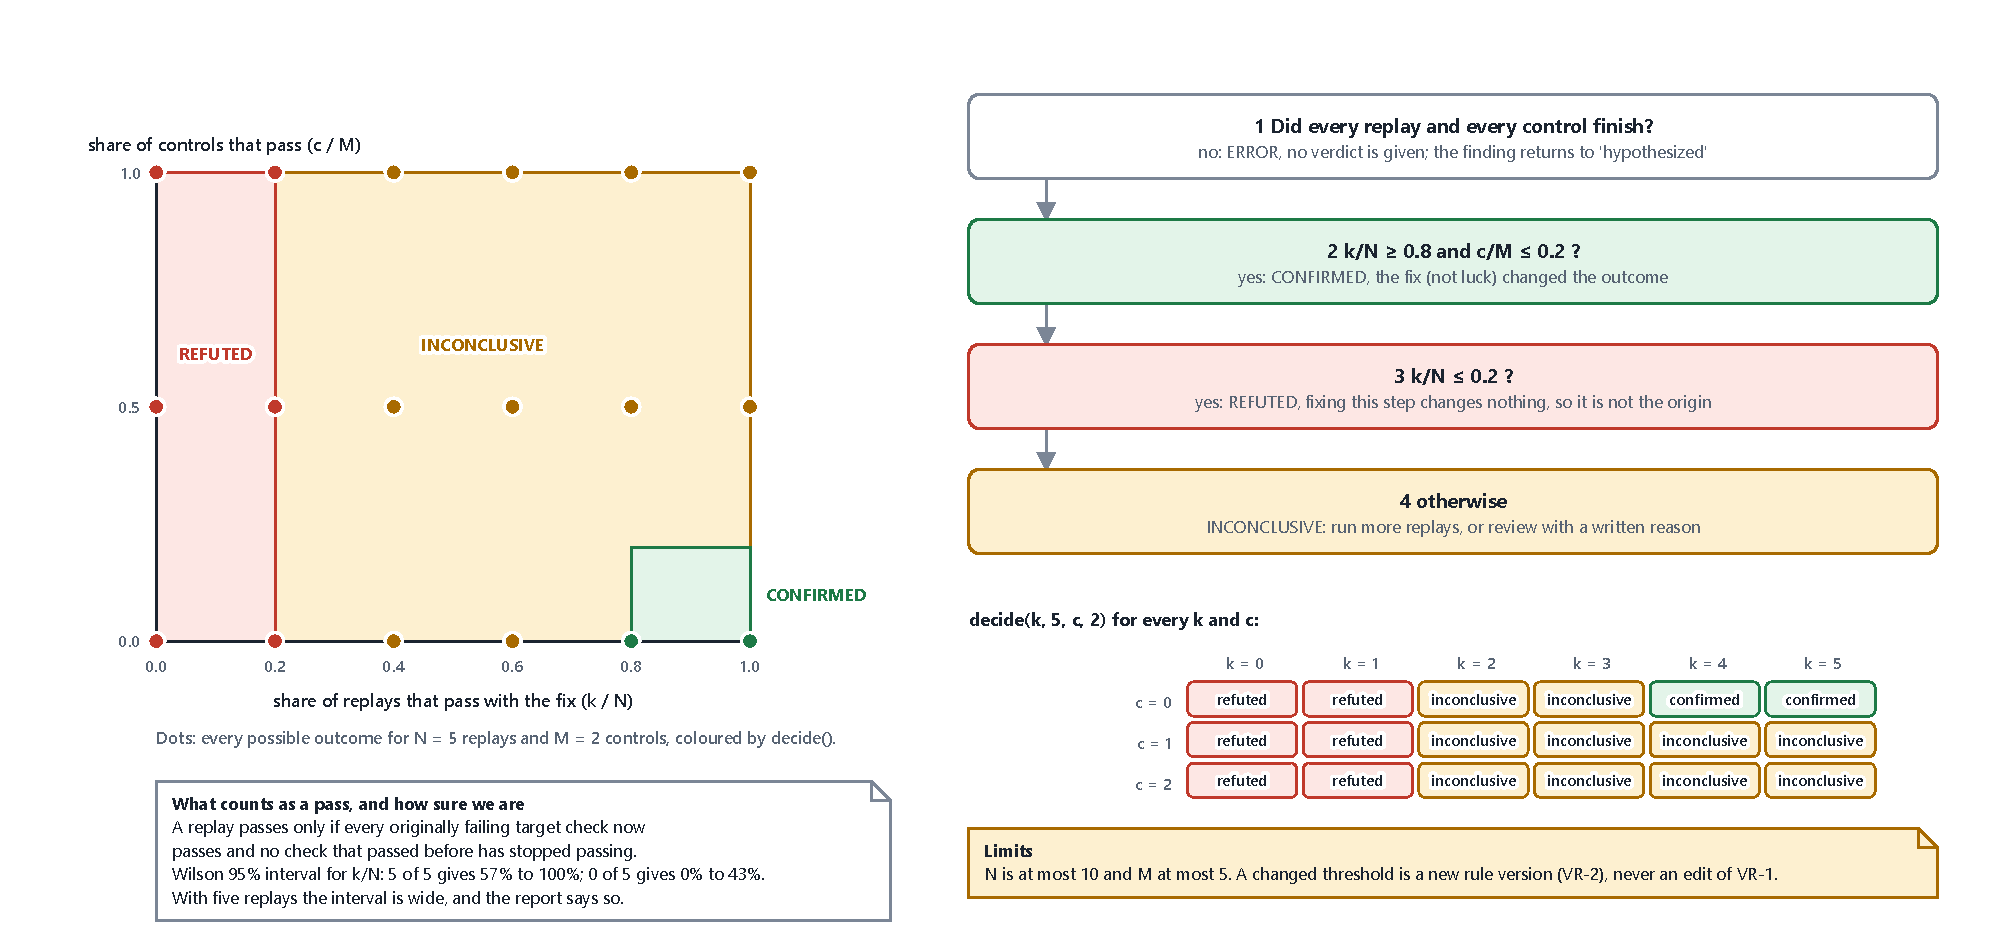
\includegraphics[width=\linewidth,height=0.42\textheight,keepaspectratio]{vr1-decision.pdf}
\caption{Verdict rule VR-1}
\label{fig:vr1}
\end{figure}


\begin{figure}[htbp]
\centering
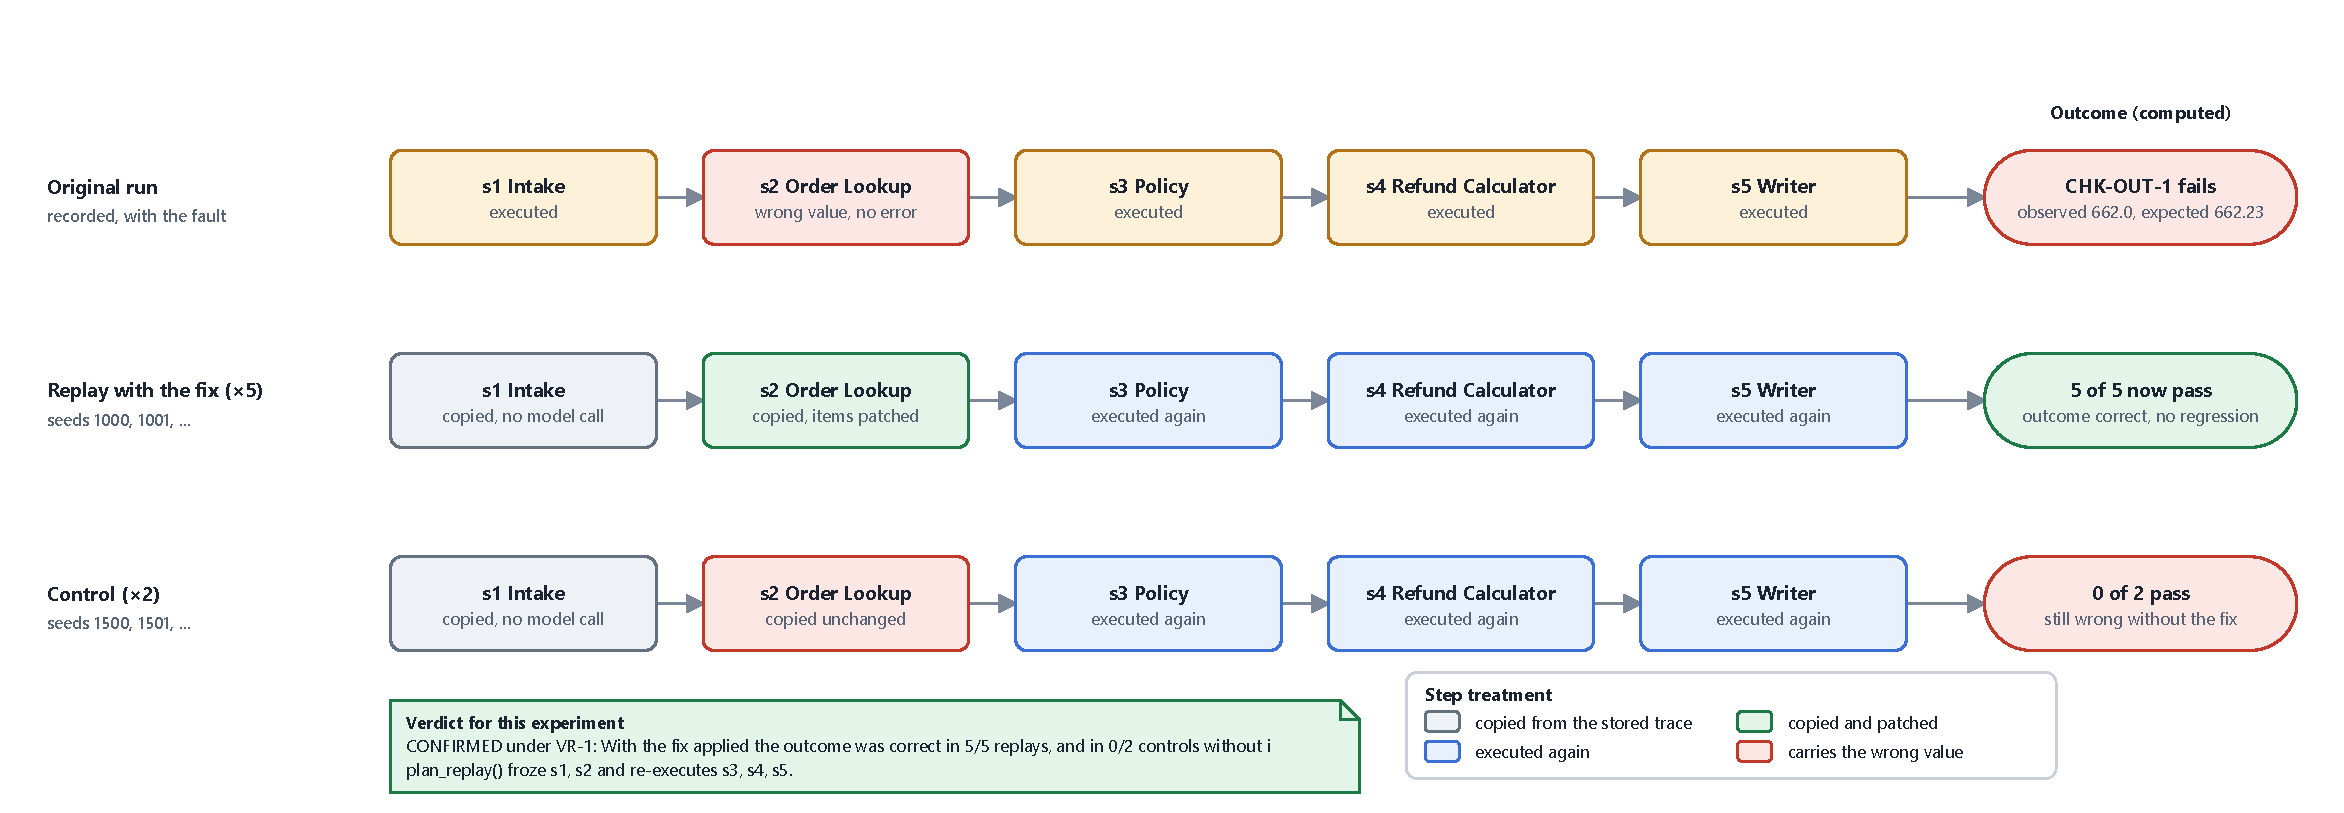
\includegraphics[width=\linewidth,height=0.42\textheight,keepaspectratio]{replay-plan.pdf}
\caption{Replay plan: correct one step, keep everything before it}
\label{fig:replay-plan}
\end{figure}


\section{Tools, Frameworks and Technologies}

Python 3.11, FastAPI, Pydantic, SQLAlchemy, uvicorn; React 19, TypeScript, Vite; SQLite (PostgreSQL supported); Ollama with llama3.2:3b; pytest, Hypothesis, Vitest, Testing Library, axe-core; ruff, mypy (strict), ESLint, bandit, pip-audit, npm audit, gitleaks; Docker and Docker Compose; GitHub Actions and GitHub Container Registry; Render. AI-assisted development (Claude Code) is disclosed in Section 8.7.

\section{Demonstration Evidence}

The product is deployed at \url{https://granite-demo.onrender.com} and runs locally from the setup steps. Screenshots of every screen, the error state and the phone layout are in \texttt{evidence/\allowbreak{}demos/\allowbreak{}} (insert the run page and finding page as figures). The demonstration script with expected values is \texttt{docs/\allowbreak{}manuals/\allowbreak{}demo-runbook.\allowbreak{}md}: run the first example with the stale-price fault; see the run completed with the Order Lookup and Writer steps failing their checks; open the finding and see Order Lookup ranked first; verify it (CONFIRMED, 5/5 fixed, 0/2 controls); verify the calculator (REFUTED); accept with a comment and download the report; then show that a clean run raises no finding and that invalid input and an unreachable model are handled.


Figures~\ref{fig:shot-list} to~\ref{fig:shot-guide} show the product during the demonstration.
\begin{figure}[htbp]
\centering
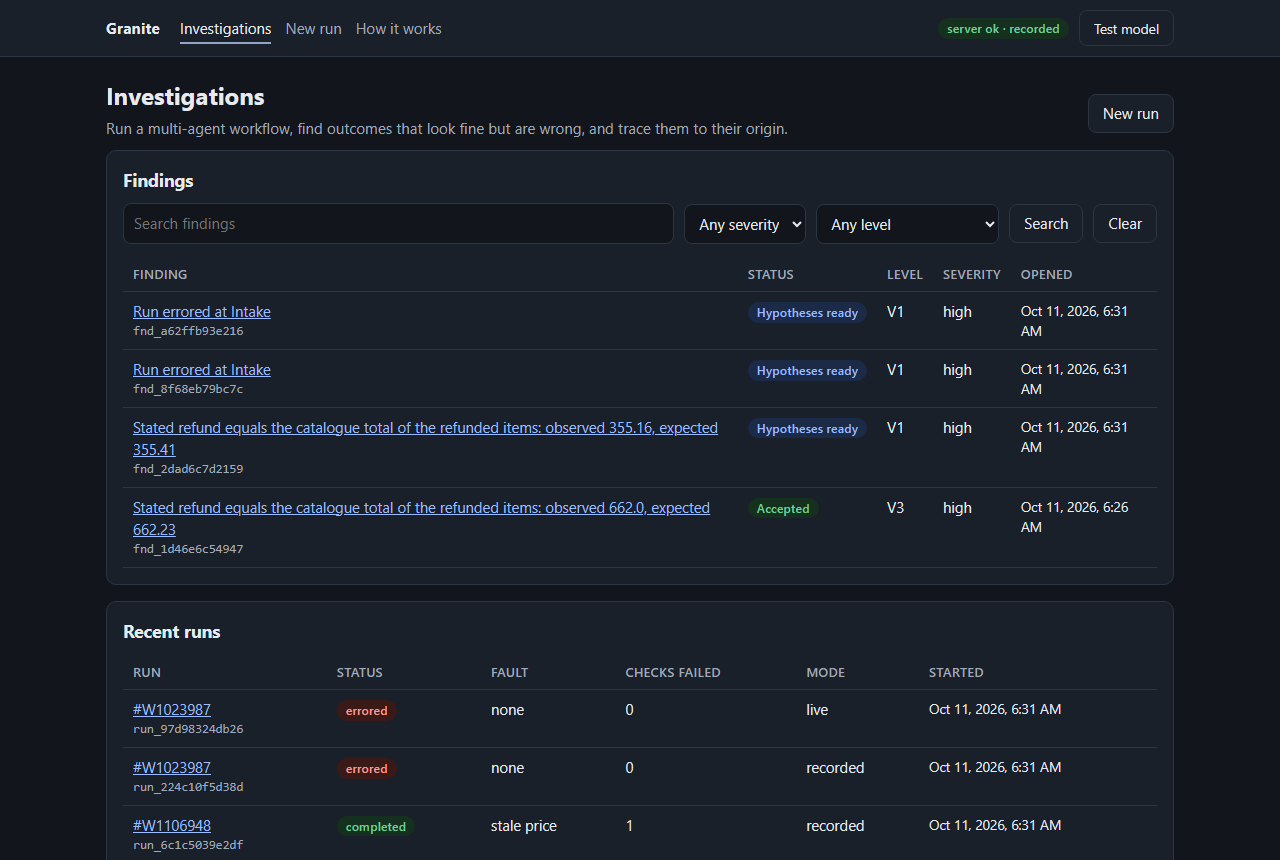
\includegraphics[width=\linewidth,height=0.42\textheight,keepaspectratio]{2026-10-11_investigations-list-filters.png}
\caption{Investigations list: earlier runs and findings, with filters and search}
\label{fig:shot-list}
\end{figure}

\begin{figure}[htbp]
\centering
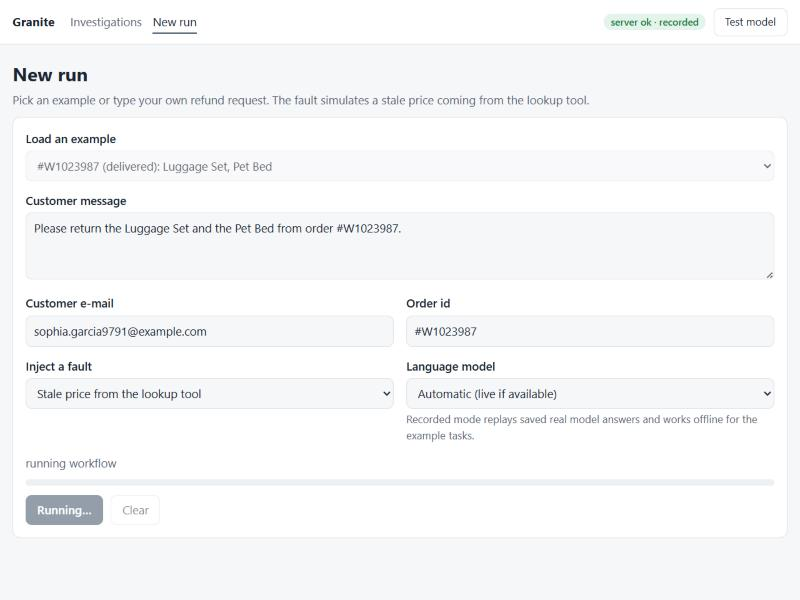
\includegraphics[width=\linewidth,height=0.42\textheight,keepaspectratio]{2026-10-07_new-run-form-running.jpg}
\caption{New run: validated input form}
\label{fig:shot-newrun}
\end{figure}


\begin{figure}[htbp]
\centering
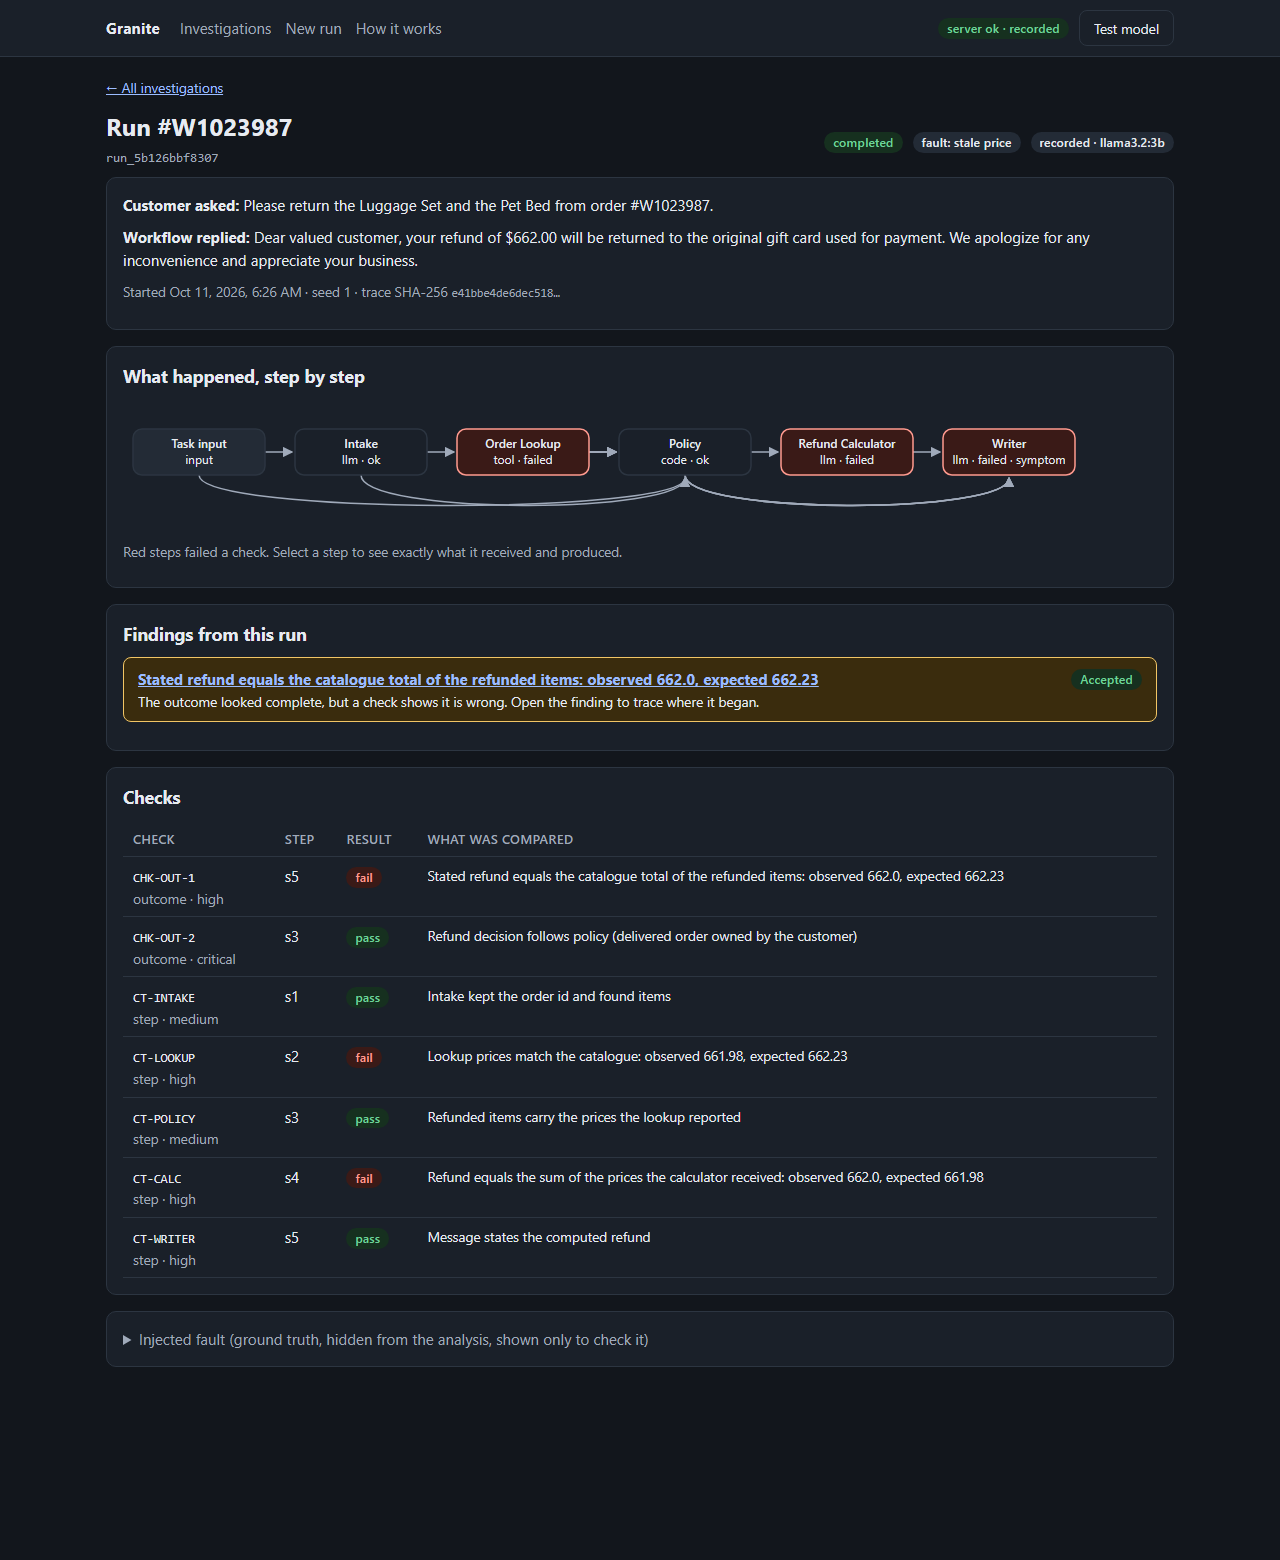
\includegraphics[width=\linewidth,height=0.42\textheight,keepaspectratio]{2026-10-11_run-detail-checks-graph.png}
\caption{Run page: pipeline graph with failed steps and the seven checks}
\label{fig:shot-run}
\end{figure}


\begin{figure}[htbp]
\centering
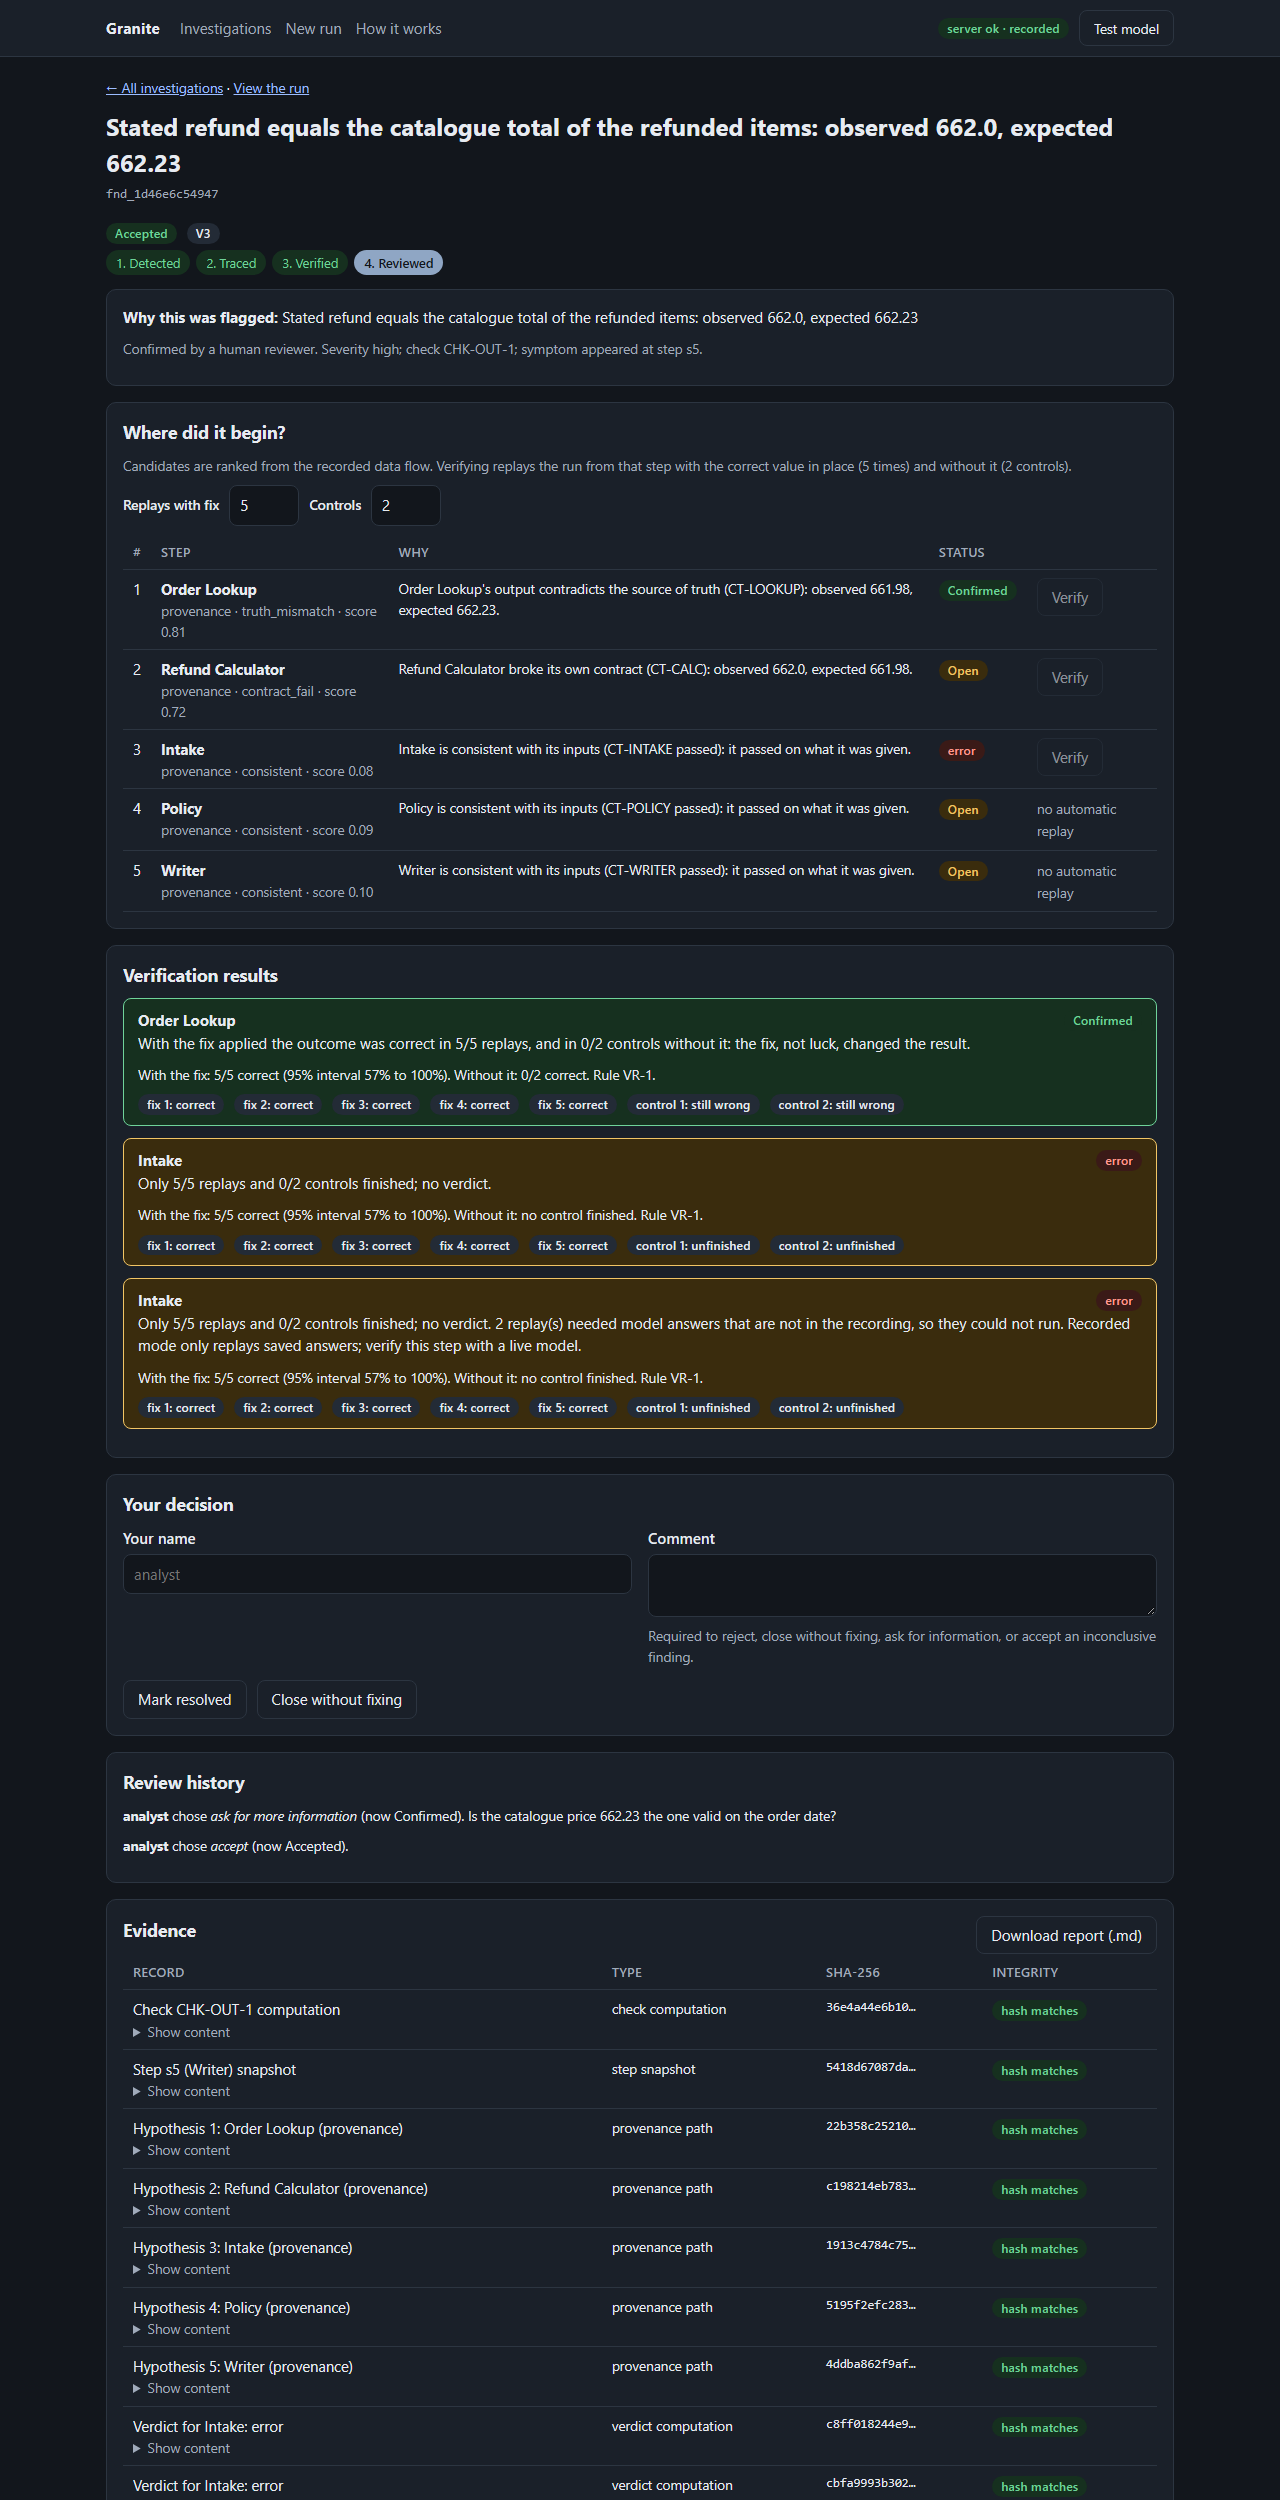
\includegraphics[width=\linewidth,height=0.62\textheight,keepaspectratio]{2026-10-11_finding-confirmed-reviewed-evidence.png}
\caption{Finding page: ranked hypotheses, verification results, review and evidence}
\label{fig:shot-finding}
\end{figure}


\begin{figure}[htbp]
\centering
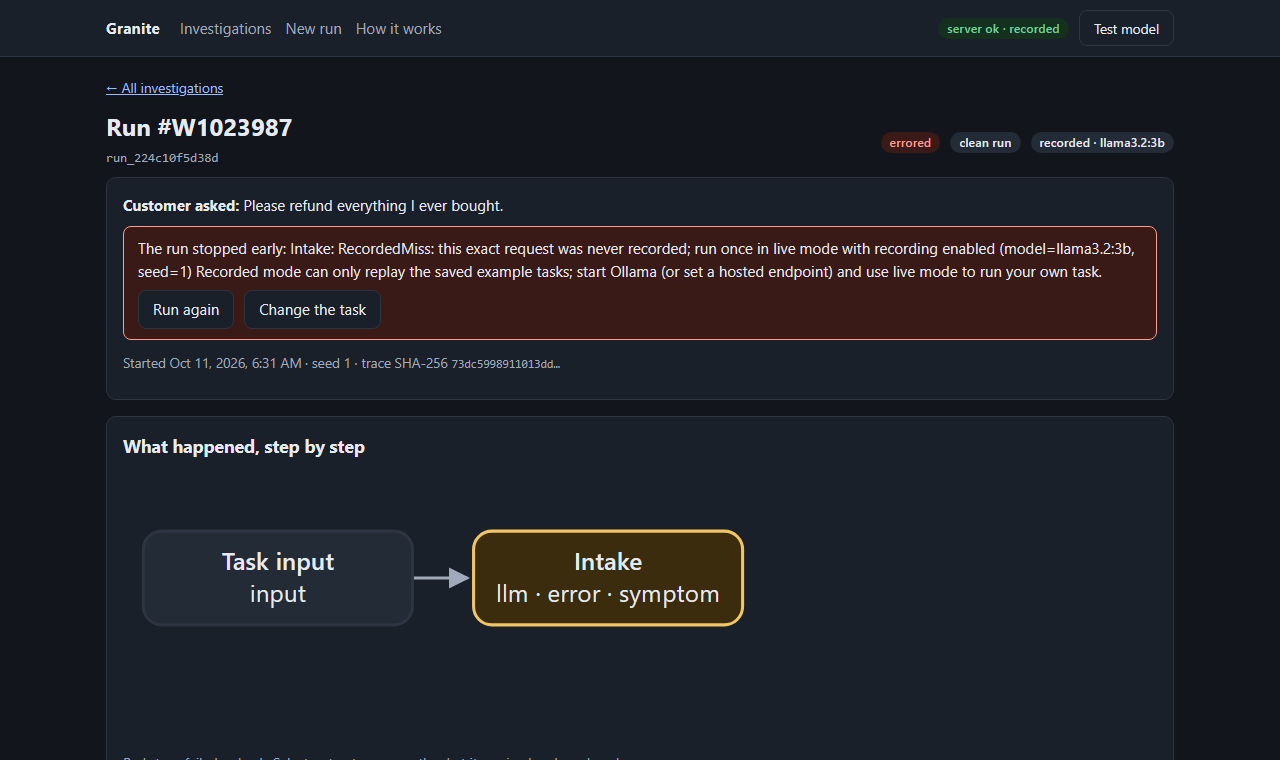
\includegraphics[width=\linewidth,height=0.42\textheight,keepaspectratio]{2026-10-11_run-errored-unrecorded-task.png}
\caption{Failure case: a run that cannot be answered ends as errored with the reason}
\label{fig:shot-error}
\end{figure}

\begin{figure}[htbp]
\centering
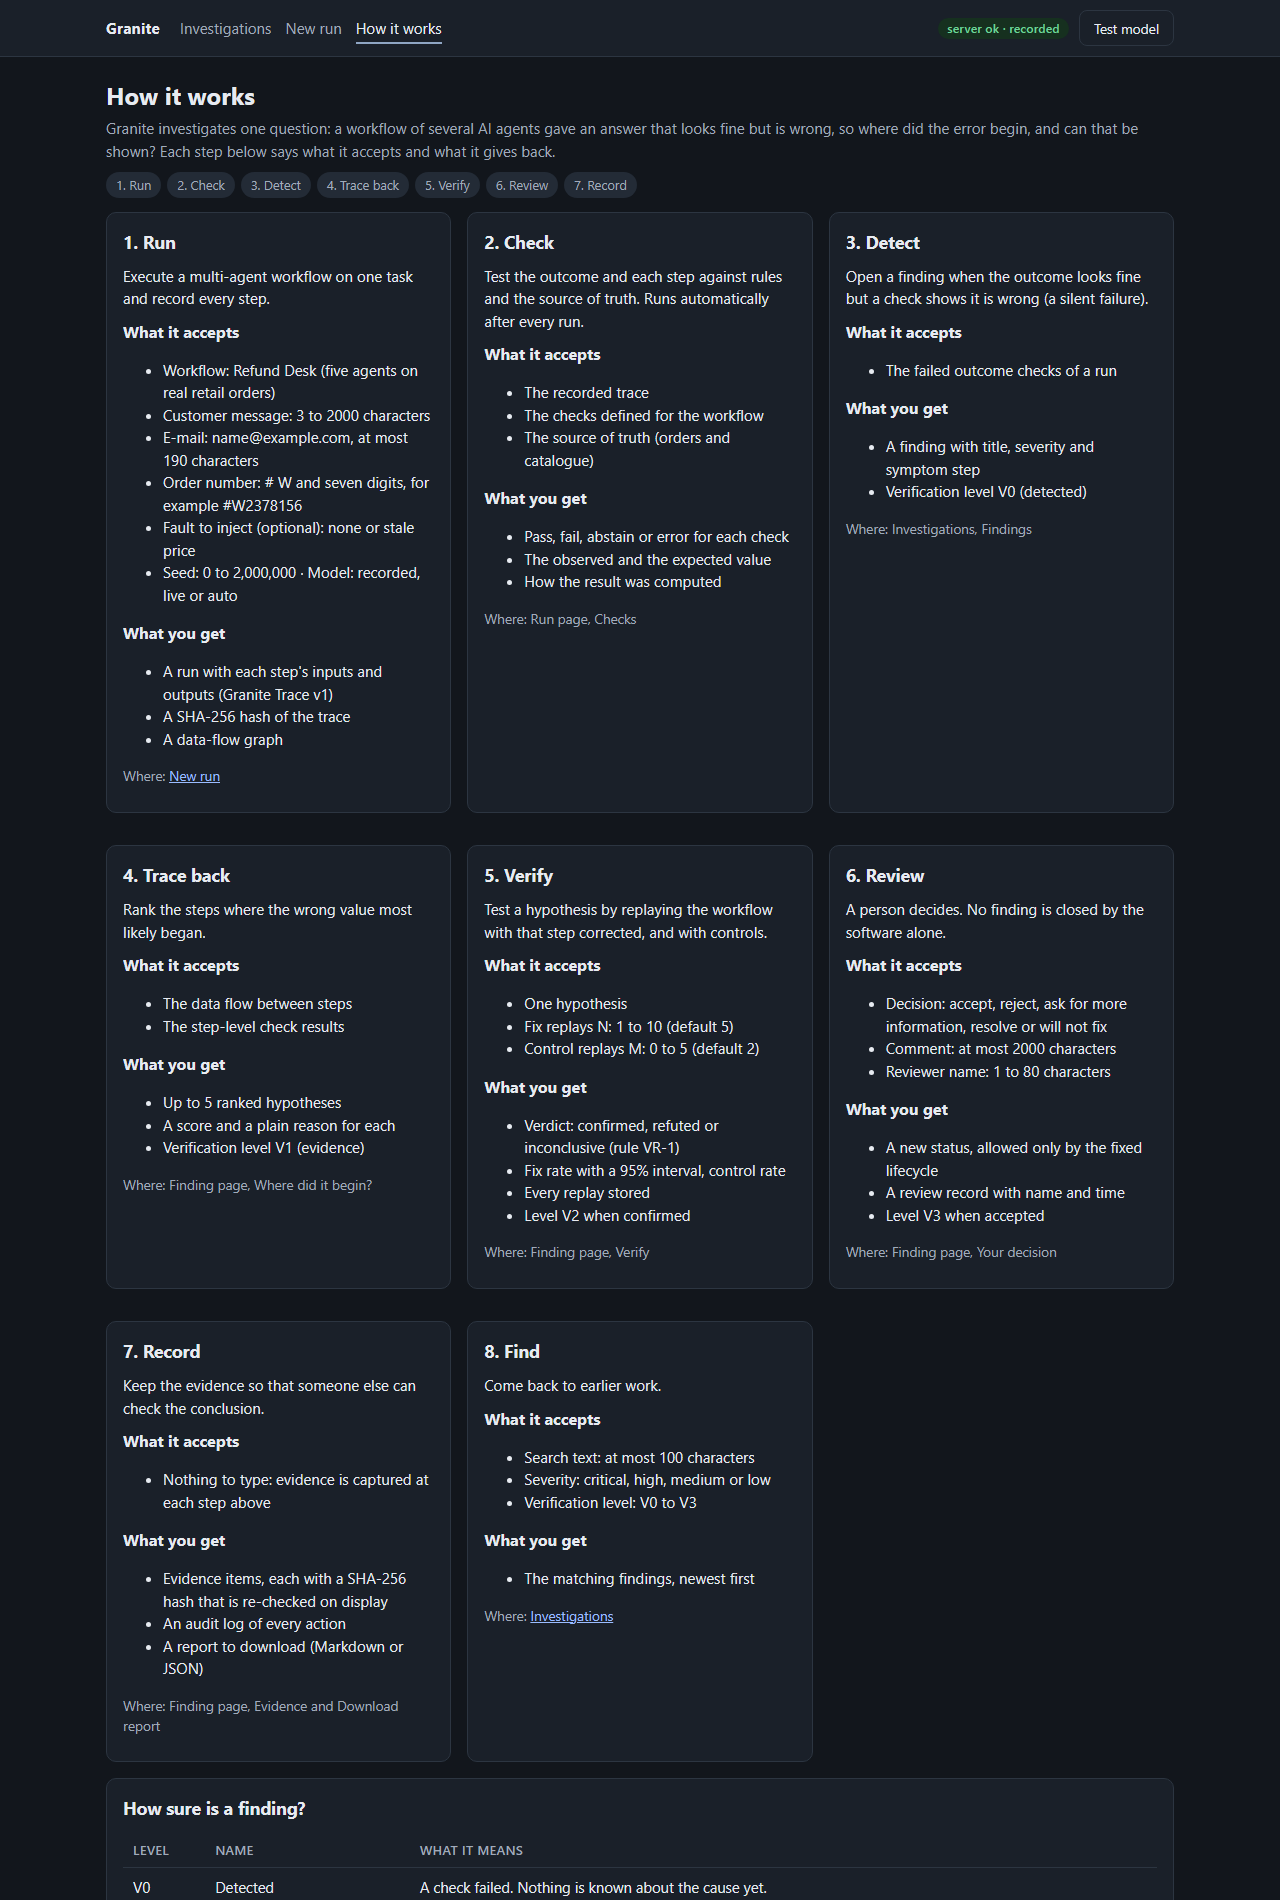
\includegraphics[width=\linewidth,height=0.42\textheight,keepaspectratio]{2026-10-11_guide-features-inputs-outputs.png}
\caption{Guide page: the eight features with their inputs and outputs (feature F8)}
\label{fig:shot-guide}
\end{figure}
\section{Iteration Outcome}

Iteration 1 met its objective: the full investigation loop works end to end on real data with a real model, is deployed, and is covered by 381 automated tests and CI. The pre-registered feasibility run met all thresholds. Shortfalls carried into Iteration 2 are redaction before storage, a usability test with outside users, fully automated deployment, and visible per-member ownership of the code.

%======================================================================================
% chapter8_testing
%======================================================================================
\chapter{Testing and Early Validation}

This chapter describes how Granite was tested and validated: the strategy, the test levels and techniques, the test cases and their results, the pre-registered feasibility validation, the edge and failure cases covered, the defects found and fixed, and what the current evidence does and does not support.

\section{Testing Strategy}

We separate three questions: \textbf{testing} asks whether Granite behaves as specified; \textbf{evaluation} asks whether it is accurate against baselines; \textbf{acceptance} asks whether users can and will use it. At Mid-1, testing is complete for the implemented slice, evaluation is a pre-registered feasibility run, and acceptance has a ready protocol. Every requirement has at least one test that can fail, failure and edge cases are tested at every level, and all suites run in CI on every push and pull request with a 90\% coverage gate.

\section{Test Levels and Techniques}

{\small
\begin{longtable}{>{\raggedright\arraybackslash\hspace{0pt}}p{0.170\linewidth}>{\raggedright\arraybackslash\hspace{0pt}}p{0.437\linewidth}>{\raggedright\arraybackslash\hspace{0pt}}p{0.200\linewidth}>{\raggedright\arraybackslash\hspace{0pt}}p{0.053\linewidth}}
\caption{Test Levels and Techniques}\label{tab:chapter8_testing-1}\\
\toprule
\textbf{Level} & \textbf{Scope} & \textbf{Tools} & \textbf{Count} \\
\midrule
\endfirsthead
\toprule
\textbf{Level} & \textbf{Scope} & \textbf{Tools} & \textbf{Count} \\
\midrule
\endhead
\bottomrule
\endlastfoot
Unit and property & Core library: check language, checks, attribution, verdict rule, lifecycle, evidence, redaction & pytest, Hypothesis & 207 \\
Unit and integration & Refund Desk steps, store, fault, verification & pytest & 49 \\
Integration & API with database, runner with recorded model, job runner & pytest, HTTP test client & 71 \\
System (black box) & User journeys and failure modes over real HTTP against a running server & pytest & 22 \\
UI component and accessibility & Screens, components, axe-core checks in light and dark & Vitest, Testing Library, axe-core & 32 \\
Static and security analysis & Lint, strict types, security, dependency vulnerabilities, secrets & ruff, mypy, ESLint, tsc, bandit, pip-audit, npm audit, gitleaks & every push \\
\end{longtable}
}

Techniques: equivalence partitioning (check statuses, fault types, input validity classes); boundary values (verdict thresholds at 0.2 and 0.8, input length limits); a decision table for VR-1 (20 rows); state-transition testing of every legal transition and several illegal ones; property-based testing (the check language never crashes on arbitrary text and never accepts forbidden syntax); error guessing (non-JSON model output, unreachable model, unrecorded task); and negative tests (clean runs must produce no findings).

\section{Test Cases}

The 22 system test cases cover three groups. \textbf{Core journeys:} full investigation of a silent failure (SYS-CORE-01); a clean run raises no alarm (02); refute a wrong hypothesis, then confirm the right one (03); the run graph marks failing steps (04); runs and findings can be found again (05); the interface is documented by the running system (06); the web interface is served by the same server (07). \textbf{Errors:} invalid input refused per field (SYS-ERR-01); requests for missing items (02); the lifecycle cannot be skipped (03); recorded mode cannot answer an unrecorded task (04); an untestable hypothesis is refused, not guessed (05); limits are enforced (06); the model is down (07). \textbf{Security and reliability:} security headers on every response (SYS-SEC-01); evidence is append-only (02); ground truth stays out of evidence (03); with a token configured only health is public (04); excessive requests are throttled (05); a restart loses nothing (SYS-REL-01); concurrent work is not lost (02); recorded runs are reproducible (03). Each case names its requirement, steps and expected result (Appendix C).

\section{Test Results}

On 11 October all 381 automated tests passed: core library 207 (97.5\% line coverage), Refund Desk 49 (95.4\%), API 71 (96.8\%), system 22 and web 32. Static analysis reported no findings. CI passed on GitHub for the latest commits, including the container build and a smoke test inside the container. Against the public deployment, the smoke test passed and the system suite gave 18 passed and 4 skipped by design (those four cases start their own server). The suites were also run on a second machine, where repetition exposed one intermittent defect (D-26, below).

\begin{figure}[htbp]
\centering
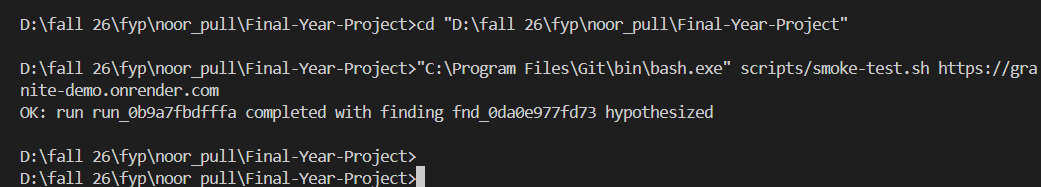
\includegraphics[width=\linewidth,height=0.42\textheight,keepaspectratio]{2026-10-11_render-smoke-test.png}
\caption{Smoke test passing against the public deployment}
\label{fig:smoke}
\end{figure}


\section{Acceptance Testing / Validation}

A feasibility validation was pre-registered before it was run: ten tasks, each run clean and with the stale-price fault, with the local model llama3.2:3b, N = 5 and M = 2, and thresholds fixed in advance. Results: the fault was detected in 10/10 faulty runs (threshold $\geq$ 90\%); there were no false alarms on clean runs (threshold 0); the true origin was ranked first in 10/10 ($\geq$ 80\%); it was CONFIRMED in 9/10 ($\geq$ 80\%); the innocent step was REFUTED in 10/10 ($\geq$ 80\%); and 20/20 runs completed ($\geq$ 95\%). The single finding on a clean run was a genuine error: the model told a customer 4,047.67 instead of 3,047.67, which Granite caught although nobody injected it.

We state the limits plainly: ten tasks, one fault type, one small model and synthetic data, so intervals are wide (the lower bound for M4 is 60\%); four tasks were not blind; attribution is easy here because the origin step has its own check; and the refutation test is weak. User acceptance testing has a ready protocol (five tasks, the SUS questionnaire, thresholds fixed in advance) and will run with three outside participants before FYP-1 Final.

\section{Edge and Failure Cases}

Tested and shown in the demonstration: a clean run produces no finding; invalid input is refused with one message per field; an unreachable model or an unrecorded task ends the run as "errored" with a reason and a retry button; verifying an innocent step gives REFUTED; a step without a repair rule cannot be verified, and the system says why; accepting before verification and rejecting without a comment are refused; hostile check expressions are rejected; tampered evidence is detected; excessive requests are throttled; and a restart marks interrupted work as failed instead of losing it. The feasibility run also exposed a real design limit: with two faults in a chain, correcting one step cannot produce a CONFIRMED verdict (D-19).

\section{Defects and Corrective Actions}

Twenty-six defects have been logged. Examples of fixed defects: the stale-price fault hit the first item instead of the requested one (D-01, fixed with a regression test); a non-ASCII token caused a server error instead of 401 (D-15); oversized request bodies were read into memory (D-16, now refused with 413); a slow health check on machines without a model (D-22, now cached); a verification with no verdict gave no reason (D-23); validator wording was shown to users (D-24); and a review decision was answered before it was saved, so an immediate next request could see the old state (D-26, found by repeating system tests on a second machine, fixed by committing before responding; the test then passed 15 of 15 runs). Open defects include the redaction gap (D-07), untested PostgreSQL (D-08), recorded answers tied to exact prompts (D-10), the two-fault limit (D-19) and rank/score disagreement for low-ranked steps (D-25), each with a plan.

\section{Current Validation Status}

The implemented slice is fully tested at every level and works on a live deployment; the feasibility run supports the claim that the run, check, trace-back and verify loop works end to end on a real small model and public data. It does not yet support claims about accuracy in general, harder faults, other workflows or usability with real users. Those are the targets of the Iteration 2 benchmark (at least 120 runs with baselines) and the usability pilot.

%======================================================================================
% chapter9_development_evidence
%======================================================================================
\chapter{Project Management and Development Evidence}

This chapter reports how the project was managed and gives the evidence behind it: work completed and remaining, individual responsibilities and contributions, repository and version-control practice, milestones, tool and AI-assisted development, external components, risks, security and privacy, and current limitations.

\section{Work Completed}

The first iteration of Granite, the core investigation slice, was completed between 6 and 11 October 2026 and is released as version 0.1.0. Granite does one job: when a workflow of several AI agents produces an answer that looks correct but is wrong, it finds the step where the error began and shows the proof. The product follows a fixed sequence of Run, Check, Detect, Trace back, Verify, Review and Record, and each stage in that sequence is a working feature.

A user can run the Refund Desk workflow, in which five agents handle a customer's refund request on real retail orders, and Granite records every step's inputs and outputs as a hashed trace. A fault such as a stale price from the order lookup can be injected before the run. After every run, seven executable checks are evaluated against a source of truth that the workflow does not control; two of these judge the final outcome and five act as contracts for individual steps. When an outcome check fails on a run that completed without any error, Granite opens a finding for a silent failure. It then traces the wrong value back through the data flow between steps and ranks the steps where it most likely entered, without using a language model. The top hypothesis can be verified by controlled replay: the workflow is re-run five times with the suspected step corrected and twice without the correction as controls, and a fixed rule (VR-1) returns CONFIRMED, REFUTED or INCONCLUSIVE. A person then accepts or rejects the finding, every decision is stored as append-only evidence with a SHA-256 hash, and the investigation can be exported as a Markdown or JSON report. Earlier runs and findings can be searched and filtered, and the product explains itself through a guide page and an API reference.

Alongside the product, the team completed a re-check of the master plan against the Mid-1 rubric, a reorganised repository with automated structure and link checks, continuous integration on GitHub Actions (first green run on 9 October), a design pack of 21 diagrams generated from the code, a suite of 22 system-level tests, setup and tool manuals, and the panel action register. On 11 October the product was deployed publicly on Render at \url{https://granite-demo.onrender.com} and verified with a smoke test and the system test suite.

All 381 automated tests pass. Their distribution is shown in Table~\ref{tab:8-1}. Lint, strict type checking, security scanning and dependency audits report no findings.

{\small
\begin{longtable}{>{\raggedright\arraybackslash\hspace{0pt}}p{0.607\linewidth}>{\raggedright\arraybackslash\hspace{0pt}}p{0.112\linewidth}>{\raggedright\arraybackslash\hspace{0pt}}p{0.171\linewidth}}
\caption{Automated test results, 11 October 2026}\label{tab:8-1}\\
\toprule
\textbf{Suite (level)} & \textbf{Tests} & \textbf{Line coverage} \\
\midrule
\endfirsthead
\toprule
\textbf{Suite (level)} & \textbf{Tests} & \textbf{Line coverage} \\
\midrule
\endhead
\bottomrule
\endlastfoot
Core library (unit, property-based) & 207 & 97.5\% \\
Refund Desk workflow (unit, integration) & 49 & 95.4\% \\
API (integration) & 71 & 96.8\% \\
System (black box over HTTP) & 22 & n/a \\
Web UI (component, accessibility) & 32 & n/a \\
\end{longtable}
}

Feasibility was checked with a pre-registered validation run on 7 October, in which the thresholds were fixed before any result was seen. Ten tasks were each run once clean and once with the injected fault, using the local model llama3.2:3b. Granite detected the fault in all ten faulty runs, raised no false alarm on the clean runs, ranked the true origin first in all ten cases, confirmed it in nine, refuted the innocent step in all ten and completed all twenty runs. Every pre-registered threshold was met. The single clean-run finding turned out to be a genuine arithmetic error made by the model, which Granite caught although nobody had injected it.

\section{Work Remaining}

Several Iteration 1 items are late or incomplete. Although the public demo is live, the continuous deployment workflow does not yet deploy automatically, because the Render deploy hook has still to be added as a repository secret. The main branch is not protected, no release tag exists, and only one of the three members has opened pull requests. No member has yet demonstrated a file-level walkthrough of their module. Redaction of personal data before storage has been written and tested but not applied, a usability check with three outside users has not been scheduled, and change record C-01 still awaits the supervisor's signature. Each of these has an owner and a date in the recovery plan: the deployment secret, branch protection and tag before the Mid-1 meeting; one reviewed pull request and a walkthrough from every member before the meeting; the usability check in Week 9; and redaction in Week 10.

Of the nineteen functional requirements set for Mid-1, fourteen are met, four are partly met and one is not met. A finding is opened for each failing outcome check rather than as one combined finding (recorded as deviation C-02h). The origin step is ranked first in ten of ten real-model tasks, but the stricter acceptance criterion of 95\% over twenty runs has not been measured. The report export lacks PDF, which is planned for FYP-1 Final, and the history view has no project filter because only one project exists. Redaction before storage (FR-SEC-01) is the requirement not yet met.

\section{Individual Responsibilities}

The three ownership areas approved at the proposal defense are unchanged and have been mapped onto the product modules. Shahoud Shahid owns Workflows, Data and Experience: the Run and Import modules, the Fault Lab and benchmark, the language-model provider layer and redaction, and the web interface. Muhammad Noor Ul Haq owns the Investigation Engine: the check language and checks engine, the trace-back attribution algorithm, and the evaluation harness with its baselines and metrics. Saif Shahzad owns Verification and Platform: replay verification and the verdict rule, the review lifecycle, reporting, the API, database and background jobs, CI/CD, deployment and security.

The writing of this report is divided equally, with each member writing the chapters closest to their own area, about a third of the report each: Shahoud Shahid writes the front matter, Chapters 1, 3, 9 and 10, and Appendices A and F; Muhammad Noor Ul Haq writes Chapters 2, 4 and 8 and Appendices B and E; and Saif Shahzad writes Chapters 5, 6 and 7 and Appendices C and D. Beyond the report, Shahoud is responsible for the vision, use cases, wireframes, user manual, usability testing and poster; Noor for the literature and product review, requirements, algorithm design and evaluation; and Saif for the architecture, data and behaviour models, test plan, CI/CD, deployment and the setup and tool manuals. Architecture decisions, integration testing, code review, ethics and defense preparation are shared, and every member is expected to demonstrate the full investigation journey alone. Table~\ref{tab:8-2} summarises accountability.

{\small
\begin{longtable}{>{\raggedright\arraybackslash\hspace{0pt}}p{0.584\linewidth}>{\raggedright\arraybackslash\hspace{0pt}}p{0.100\linewidth}>{\raggedright\arraybackslash\hspace{0pt}}p{0.084\linewidth}>{\raggedright\arraybackslash\hspace{0pt}}p{0.093\linewidth}}
\caption{Responsibility matrix (R responsible, A accountable, C consulted, I informed)}\label{tab:8-2}\\
\toprule
\textbf{Deliverable} & \textbf{Shahoud} & \textbf{Noor} & \textbf{Saif} \\
\midrule
\endfirsthead
\toprule
\textbf{Deliverable} & \textbf{Shahoud} & \textbf{Noor} & \textbf{Saif} \\
\midrule
\endhead
\bottomrule
\endlastfoot
Runner, workflows, faults, SDK & R/A & C & C \\
Checks, attribution, evaluation & C & R/A & C \\
Verification, review, API/DB, CI/CD, deployment & C & C & R/A \\
UI consistency, report integration & R/A & R & R \\
Supervisor minutes, Form 10, milestone log & R/A & I & I \\
Form 13 and AI usage log & R & R & R/A \\
Release tagging & C & C & R/A \\
\end{longtable}
}

\section{Contribution of Each Team Member}

Contribution is reported as it appears in the repository. Excluding merges, the main branch holds 82 commits: 40 from Shahoud, 40 from Noor and 1 from Saif, who also made seven merge commits on the proposal-stage branch. The history falls into three phases. During the proposal stage, from late August to the defense on 11 September, the work was shared: Shahoud led the early literature and proof-of-concept spikes, and Noor produced most of the proposal deck and defense preparation. No commits were made between 14 September and 4 October. Between 6 and 11 October the entire product was built in AI-assisted sessions run by Shahoud and committed from his account.

Since 11 October Noor has deployed the product, verified it against the public URL, and opened the project's first two pull requests: one recording the deployment and its evidence, and one fixing a defect (D-26) found by repeating the system tests on a second machine. The planned ownership described in Section 8.3 is therefore not yet reflected in the commit history for the implementation. The team recognises this as the main process weakness of Iteration 1 and has adopted the recovery steps in Section 8.2, in which each member makes real changes to their own module through reviewed pull requests from their own account.

\section{Repository and Version Control Evidence}

The code is kept in a private GitHub repository, Shahoud867/Final-Year-Project, with main as the default branch. Commit messages follow the Conventional Commits format, for example \texttt{feat(\allowbreak{}core): \ldots{}} or \texttt{docs(\allowbreak{}deploy): \ldots{}}. Continuous integration runs on every push and pull request in four jobs. The Python job runs ruff, mypy in strict mode, pytest with a 90\% coverage gate, bandit and pip-audit. The web job runs ESLint, the TypeScript compiler, Vitest, a production build and npm audit. A secret scan runs gitleaks, and a container job builds the Docker image and smoke-tests it. The continuous deployment workflow builds and tests the image, publishes it to the GitHub Container Registry, triggers Render and smoke-tests the public URL. Its first run on 11 October published the image, and the deploy step will run once the hook secret is configured.

The agreed branching strategy (ADR-010) is that nobody pushes to main. Each change is made on a short-lived branch named by its type (feat, fix, docs or chore), opened as a pull request, checked by CI and reviewed by another member before a squash merge. Milestones are marked by tags such as v0.1.0-mid1 and v0.2.0-final1, and pushing a tag creates a GitHub Release with a tagged container image. Up to 11 October the history shows direct pushes to main. The first two pull requests were opened on 11 October, and branch protection and the first tag are scheduled before the Mid-1 meeting.

\section{Milestones and Commit Evidence}

The proposal was approved at the defense on 11 September with five panel comments. On 6 October the master plan was revised to version 1.1, the repository was reorganised and the core library and Refund Desk workflow were working. On 7 October the API, web interface, CI definition and pre-registered feasibility run were completed. The code reached GitHub on 9 October, when the first CI run passed, including the container build and smoke test. On 11 October the design pack, system tests, deployment workflow, coding standards and guide page were added and the registers were re-checked. On the same day the public demo went live, and defect D-26 was found and fixed. Each milestone is backed by a commit, a CI or CD run, or an evidence file in the repository.

The core slice planned for Week 8 was delivered between 6 and 11 October. The items delivered late are fully automated deployment, branch protection, the release tag, pull requests from every member and the code walkthroughs, all covered by the recovery plan in Section 8.2.

\section{Tools and Tool-Assisted Development}

Granite is written in Python 3.11 with FastAPI, SQLAlchemy and Pydantic on the server, and React with TypeScript and Vite in the browser. Testing uses pytest, Hypothesis for property-based tests, Vitest, Testing Library and axe-core for accessibility. Code quality and security are enforced with ruff, mypy, ESLint, bandit, pip-audit, npm audit and gitleaks. The system is packaged with Docker, built and deployed through GitHub Actions and hosted on Render. The Refund Desk's language-model steps run on llama3.2:3b through Ollama.

Generative AI tools were used throughout and are disclosed in full in the AI usage log and Form 13. During the proposal stage a general-purpose AI assistant helped with literature-gap synthesis, planning documents, the eight proof-of-concept spike scripts and defense material. The team ran every spike, inspected its output against ground truth and corrected several errors this way, including a scoring bug and a mislabelled preprint. The implementation of Iteration 1, from 6 to 11 October, was carried out with Claude Code, an AI coding agent. This covered the core library, workflow, API, web interface, tests, CI/CD, diagrams and manuals, and is classed as core-assist at its upper bound. The design it implemented (the verdict rule, the attribution weights, the check-language limits, the state machine and the evaluation protocol) was specified by the team in the master plan before any coding. Its output was validated by running it: the automated tests, strict type checks, security scans, a run on a real local model, a browser walkthrough of the full journey and the pre-registered feasibility run. The deployment verification and the D-26 fix after 11 October were also AI-assisted, with the checks run by Noor and the fix submitted for review as a pull request. Ollama and llama3.2:3b form part of the system under test rather than of Granite's reasoning, because the checks, attribution and verdict are deterministic code. The team acknowledges that each member's ability to explain, modify and defend the AI-assisted code in their own module has still to be demonstrated, and this is scheduled before the evaluation.

\section{External Components and Dependencies}

Granite depends on a small number of permissively licensed components. The distributed runtime consists of Pydantic, FastAPI, SQLAlchemy and React, all under the MIT licence, and uvicorn under BSD-3-Clause. Development and test tools such as pytest, ruff, mypy, Vite and ESLint are MIT or Apache-2.0. Hypothesis and axe-core are under MPL-2.0, but they are used unmodified for testing only and are not shipped. The Refund Desk's customers, orders and product catalogue are a 75-order subset of the tau-bench retail dataset~\cite{taubench}, published by Sierra under the MIT licence. This synthetic data also serves as the source of truth for the checks. Ollama (MIT) runs the local model, and the Llama 3.2 3B model is covered by Meta's Llama 3.2 Community License. The weights are not distributed; only the model's recorded answers are, so the demo runs without a model. The public demo is hosted on Render's free plan, and container images are stored in the GitHub Container Registry. Two licensing questions remain open: choosing a licence for Granite itself, and confirming the Llama 3.2 terms for the recorded answers.

\section{Risks and Mitigation}

The project keeps a register of thirty risks, reviewed weekly. Table~\ref{tab:8-3} lists the most significant.

{\small
\begin{longtable}{>{\raggedright\arraybackslash\hspace{0pt}}p{0.353\linewidth}>{\raggedright\arraybackslash\hspace{0pt}}p{0.032\linewidth}>{\raggedright\arraybackslash\hspace{0pt}}p{0.032\linewidth}>{\raggedright\arraybackslash\hspace{0pt}}p{0.443\linewidth}}
\caption{Principal risks}\label{tab:8-3}\\
\toprule
\textbf{Risk} & \textbf{P} & \textbf{I} & \textbf{Mitigation} \\
\midrule
\endfirsthead
\toprule
\textbf{Risk} & \textbf{P} & \textbf{I} & \textbf{Mitigation} \\
\midrule
\endhead
\bottomrule
\endlastfoot
A member cannot explain AI-assisted code ("sudden code volume") & H & H & Small pull requests, owner-written tests, walkthrough drills; cut code to what is understood \\
Uneven contribution visible in the repository & H & H & Each member owns a module and chapters and commits through reviewed pull requests \\
Reviewers consider the work already done by DoVer or commercial tools & H & H & Honest comparison; contribution is controlled replay with controls, executable checks and self-hosting; measure the delta \\
Language-model replays too unstable, giving inconclusive verdicts & M & H & Low temperature, structured outputs, deterministic tools; increase N; report instability \\
Free hosting sleeps or changes during a demo & M & H & Wake the site beforehand; laptop or Docker Compose fallback \\
Feature creep & M & H & Frozen MoSCoW priorities; changes need a change record \\
Report diverges from the code & M & H & Diagrams generated from code and checked in CI \\
Users still find the interface unclear & M & H & Guide page, plain wording, usability pilot \\
Sandbox escape through check expressions & L & H & AST whitelist, size limits, attack tests, security scan \\
Real personal data uploaded to the demo & L & H & Synthetic data only, recorded mode, input limits \\
\end{longtable}
}

\section{Security and Privacy Considerations}

Granite's main attack surface is the check language, because checks are expressions that the server evaluates. Instead of Python's \texttt{eval}, the project uses its own evaluator built on Python's syntax tree. It accepts only a whitelist of node types and a fixed list of functions, and limits each expression to 500 characters, 150 syntax nodes and a depth of 14. Twenty-five hostile expressions are tested and rejected, and property-based tests confirm that arbitrary input never crashes the compiler. Every user input is typed and bounded, unknown fields are refused and request bodies over 256 KB are rejected. Evidence records are append-only and carry a SHA-256 hash that is re-checked when read, so tampering is detectable. Attribution never has access to the injected fault's ground truth. An optional access token closes every endpoint except the health check, state-changing requests are limited to 120 per minute, and every response carries security headers. Secrets are kept only in GitHub and Render settings, a secret scan runs in CI, and dependencies are audited on every push. Each of these controls is covered by an automated test.

On privacy, the public demo uses only synthetic data and recorded model answers. One requirement is not yet met: personal data in traces is stored without redaction (FR-SEC-01), because verification replays need the original input. A redactor exists and is tested, and a token-vault design that resolves the conflict is planned for Week 10. Ethically, faults are injected only into the project's own workflows, findings are advisory with a person making the final decision, dataset licences are recorded, and usability participants will give written consent.

\section{Current Limitations}

The evidence so far is narrow. Granite has been demonstrated on one workflow, one fault type and one small model, and the feasibility run covered only ten tasks, so its confidence intervals are wide; the lower bound for confirmed origins is 60\%. Four of the ten tasks were not blind, and no baseline comparison has been made yet. Attribution is easier than usual in this workflow, because the origin step has its own check and therefore leaves direct evidence. Workflows without step checks fall back to a structural ranking that has not been tested. The refutation test is also weak, since correcting the calculator cannot repair a wrong price.

The validation exposed one design limit. When a second fault exists further down the chain, correcting a single step cannot produce a confirmed verdict; this happened once, when the model also mis-added two prices (D-19), and resolving it needs a new version of the verdict rule. The small model makes arithmetic slips in roughly one clean run in ten. These are real failures that Granite caught, not defects in Granite. For low-ranked hypotheses, rank and score can disagree (D-25), although the top ranks are unaffected.

On the engineering side, personal data is not yet redacted before storage, PostgreSQL has not been tested and there is no migration tool, the recorded model answers must be re-recorded after any prompt change, and the rate limiter works per process. Trace import, a second workflow, a check editor, fix suggestions and PDF export are not yet built. The free hosting instance sleeps when idle and resets its database on every deploy. Finally, the tests and the code were produced by the same AI-assisted process, so high coverage shows that the code does what was intended, not that the intent is correct.

%======================================================================================
% chapter10_fyp2_plan
%======================================================================================
\chapter{Remaining FYP Plan}

This chapter sets out the plan for the rest of the project: the remaining scope and features, the iterations still to come, how they will be implemented, tested and deployed, the timeline to FYP-2, and the expected final deliverables.

\section{Remaining Scope}

Granite's full scope is eight product modules. Run executes a multi-agent workflow and records its trace. Import brings in traces from other tools through file upload, a Python SDK and framework adapters. Check evaluates executable checks and turns silent failures into findings. Trace back ranks origin hypotheses. Verify tests a hypothesis by controlled replay. Review and Resolve covers the human decision, fix suggestions, recovered runs and a library of known fixes. Report provides exports, regression tests and history. Fault Lab and Evaluation generates labelled benchmark runs and measures the system against baselines.

Iteration 1 delivered the core path of Run, Check, Trace back, Verify, Review and Report. The remaining scope is the Import module, the second half of Review and Resolve, the PDF and regression exports, and the whole of Fault Lab and Evaluation. Several things are excluded from the FYP altogether: a multi-tenant SaaS product with billing, Kubernetes or message queues, applying fixes automatically to a user's production system, training custom models, benchmarking across seven frameworks, a preventive classifier, and real customer data on the public demo.

\section{Remaining Modules and Features}

The remaining features are prioritised by milestone using MoSCoW. The Must items for FYP-1 Final are:

\begin{itemize}
\item trace import using the Granite Trace v1 format
\item a second workflow based on GSM8K maths problems
\item a Fault Lab with three fault types and clean controls
\item a Python SDK with a LangGraph adapter
\item LLM-generated fix suggestions, each verified as a fix experiment
\item recovered runs that apply a verified fix
\item export of a finding as a regression test
\item redaction of personal data
\item PDF reports
\item a first version of the evaluation module
\end{itemize}

For FYP-2 Mid, the CrewAI adapter and an LLM second-opinion hypothesis (a lightweight ErrorProbe reproduction) become Musts and the evaluation module reaches its full version. A known-fix library, GitHub login with reviewer identity, and retention controls are Should items for FYP-2. Notifications are a Could item, and support for further frameworks, a seven-framework compatibility layer and a leaderboard are left for future work.

\section{Remaining Iterations}

Three iterations remain. Iteration 2, "breadth and inputs", runs from Week 9 to Week 15 of FYP-1 and ends with release 0.2.0 at FYP-1 Final. Its goal is for about half of the committed effort to be implemented, with the core scenario working on real inputs from two sources (a live run and an imported trace), the comparison baseline measured, the deployment installed by someone other than its author, and the FYP-2 evaluation plan written. Iteration 3, "integration and evaluation", covers the first eight weeks of FYP-2. It adds the CrewAI adapter, the known-fix library, authentication, the LLM second opinion and a benchmark of at least 300 runs, and ends with release 0.5.0 at FYP-2 Mid. Iteration 4, "hardening and user acceptance", runs to the end of FYP-2 and covers acceptance testing with users, fixes and handover, ending with release 1.0.0 at FYP-2 Final.

\section{Implementation Plan}

Iteration 2 is planned week by week, with each member working in their own area.

{\small
\begin{longtable}{>{\raggedright\arraybackslash\hspace{0pt}}p{0.039\linewidth}>{\raggedright\arraybackslash\hspace{0pt}}p{0.261\linewidth}>{\raggedright\arraybackslash\hspace{0pt}}p{0.286\linewidth}>{\raggedright\arraybackslash\hspace{0pt}}p{0.274\linewidth}}
\caption{Implementation Plan}\label{tab:chapter10_fyp2_plan-1}\\
\toprule
\textbf{Week} & \textbf{Shahoud} & \textbf{Noor} & \textbf{Saif} \\
\midrule
\endfirsthead
\toprule
\textbf{Week} & \textbf{Shahoud} & \textbf{Noor} & \textbf{Saif} \\
\midrule
\endhead
\bottomrule
\endlastfoot
9 & Trace import with a validation report & Check editor backend; fix D-25 & Resume interrupted experiments \\
10 & Two more fault types; personal-data redaction & Check editor interface; cycle bound in attribution & Fix suggestion and fix experiments \\
11 & SDK and LangGraph adapter & Second workflow's checks; metamorphic tests & Recovered runs; regression-test export \\
12 & Fault Lab batch generation & Evaluation harness with last-agent and LLM-judge baselines & PDF reports; release pipeline; PostgreSQL testing \\
13 & Benchmark v0 of at least 120 runs & Run evaluation v0; label 50 natural failures & Performance measurement; accessibility pass \\
14 & Help page; SDK quickstart; UI fixes from the pilot & Evaluation screen & Install by a non-owner; rollback test \\
\end{longtable}
}

In parallel, the team will act on the Mid-1 feedback in Week 9, interview stakeholders from Week 9, submit the poster in Week 13 after a usability pilot, and draft report version 2.0 in Week 14. Week 10 is kept light for sessional exams. The SDK and adapter work in Week 11 carries the highest technical risk and will be cut back to the SDK alone if it falls behind.

All work follows the branching method described in Section 8.5. Every member opens pull requests from their own account, every pull request is reviewed by another member, and owners write the tests for their own code. A weekly owner demo, in which each member shows their own increment, doubles as rehearsal for the walkthrough the handbook requires. For the check, attribution and verification code, each owner must be able to explain it, propose an alternative, predict what breaks if it is removed, and modify it live.

\section{Testing and Validation Plan}

Testing, evaluation and acceptance are treated as three separate questions: whether the system behaves as specified, whether it performs well against baselines, and whether real users would adopt it.

Testing continues at every level already in place. Unit tests cover the core library, services and components, with coverage held above the 90\% gate in CI. Integration tests require at least one success case and one failure case for every API endpoint. Component and accessibility tests cover the web interface. The system suite runs the user journeys against the deployed URL, and browser automation is planned. Regression testing runs everything on each pull request, together with a nightly recorded mini-benchmark that fails the build if origin accuracy drops by more than five points. Performance tests check the response-time requirements, and security tests cover the check-language attack set, input fuzzing, secrets, dependency audits and redaction. The techniques used include equivalence partitioning, boundary values at the verdict thresholds, a twenty-row decision table for the verdict rule, state-transition testing of every legal and illegal finding transition, property-based tests, metamorphic tests of attribution invariances and negative tests in which clean controls must produce no findings.

Evaluation will grow through three benchmark versions. Version 0, at FYP-1 Final, has at least 120 runs. Version 1, at FYP-2 Mid, has at least 300, and version 2 may reach 500 at FYP-2 Final. Each version will contain 20\% clean controls, three fault types, two workflows and at least two runtimes. A further 50 natural failures will be labelled independently by two members, with inter-rater agreement reported, and a subset of at least 30 cases from the Who\&When benchmark will be used for the language-model attribution track. Granite's provenance attribution will be compared against blaming the last agent, an LLM judge reading the whole trace, and, at FYP-2 Mid, a lightweight ErrorProbe reproduction. Ablations will vary the number of replays and controls and remove the regression guard. Results will carry bootstrap 95\% confidence intervals with fixed seeds, and each analysis will be frozen and pre-registered before it is run, as the Mid-1 feasibility run was.

Acceptance will be tested in two stages. A pilot with three peers takes place before FYP-1 Final. Full acceptance testing in FYP-2 will involve five to eight participants, including alumni developers, AI-course students and another FYP team, who are declared as proxies for real users. Sessions will be supervised, last 45 minutes and take place with consent. They will measure task completion, time, errors, assistance needed, the System Usability Scale and time to first finding. Every issue raised will be recorded as fixed or deferred, with a reason.

\section{Deployment Plan}

The public demo has run on Render's free plan at \url{https://granite-demo.onrender.com} since 11 October. It was created from the repository's render.yaml blueprint as a Docker service in recorded model mode, with a health check and automatic deploys switched off, so that only code that has passed CI is deployed. Deployment is driven by the continuous delivery workflow: after CI passes on main, the container image is built, smoke-tested and published, Render is triggered through its deploy hook, and the public URL is smoke-tested again. The only step remaining is to add the deploy hook to the repository's secrets.

The project uses four environments. Developers run Granite locally or with Docker Compose, using Ollama or recorded answers. CI runs on GitHub's runners in recorded mode, and the public demo runs on Render. As a self-hosted product, Granite can be run on any machine with Docker Compose and a local Ollama model, following the setup manual. The demo currently stores its data in SQLite on temporary disk; PostgreSQL support will be tested in Week 12, before any shared deployment. Before FYP-1 Final, the system will be installed from the setup manual by someone who is not its author, a rollback will be tested and every release will be recorded in the deployment record. On each evaluation day the hosted instance will be woken in advance, with a laptop instance as a fallback; because recorded mode needs no network access to a model, the fallback is reliable.

Figure~\ref{fig:deployment} shows the deployment, and Figure~\ref{fig:render} the live service.

\begin{figure}[htbp]
\centering
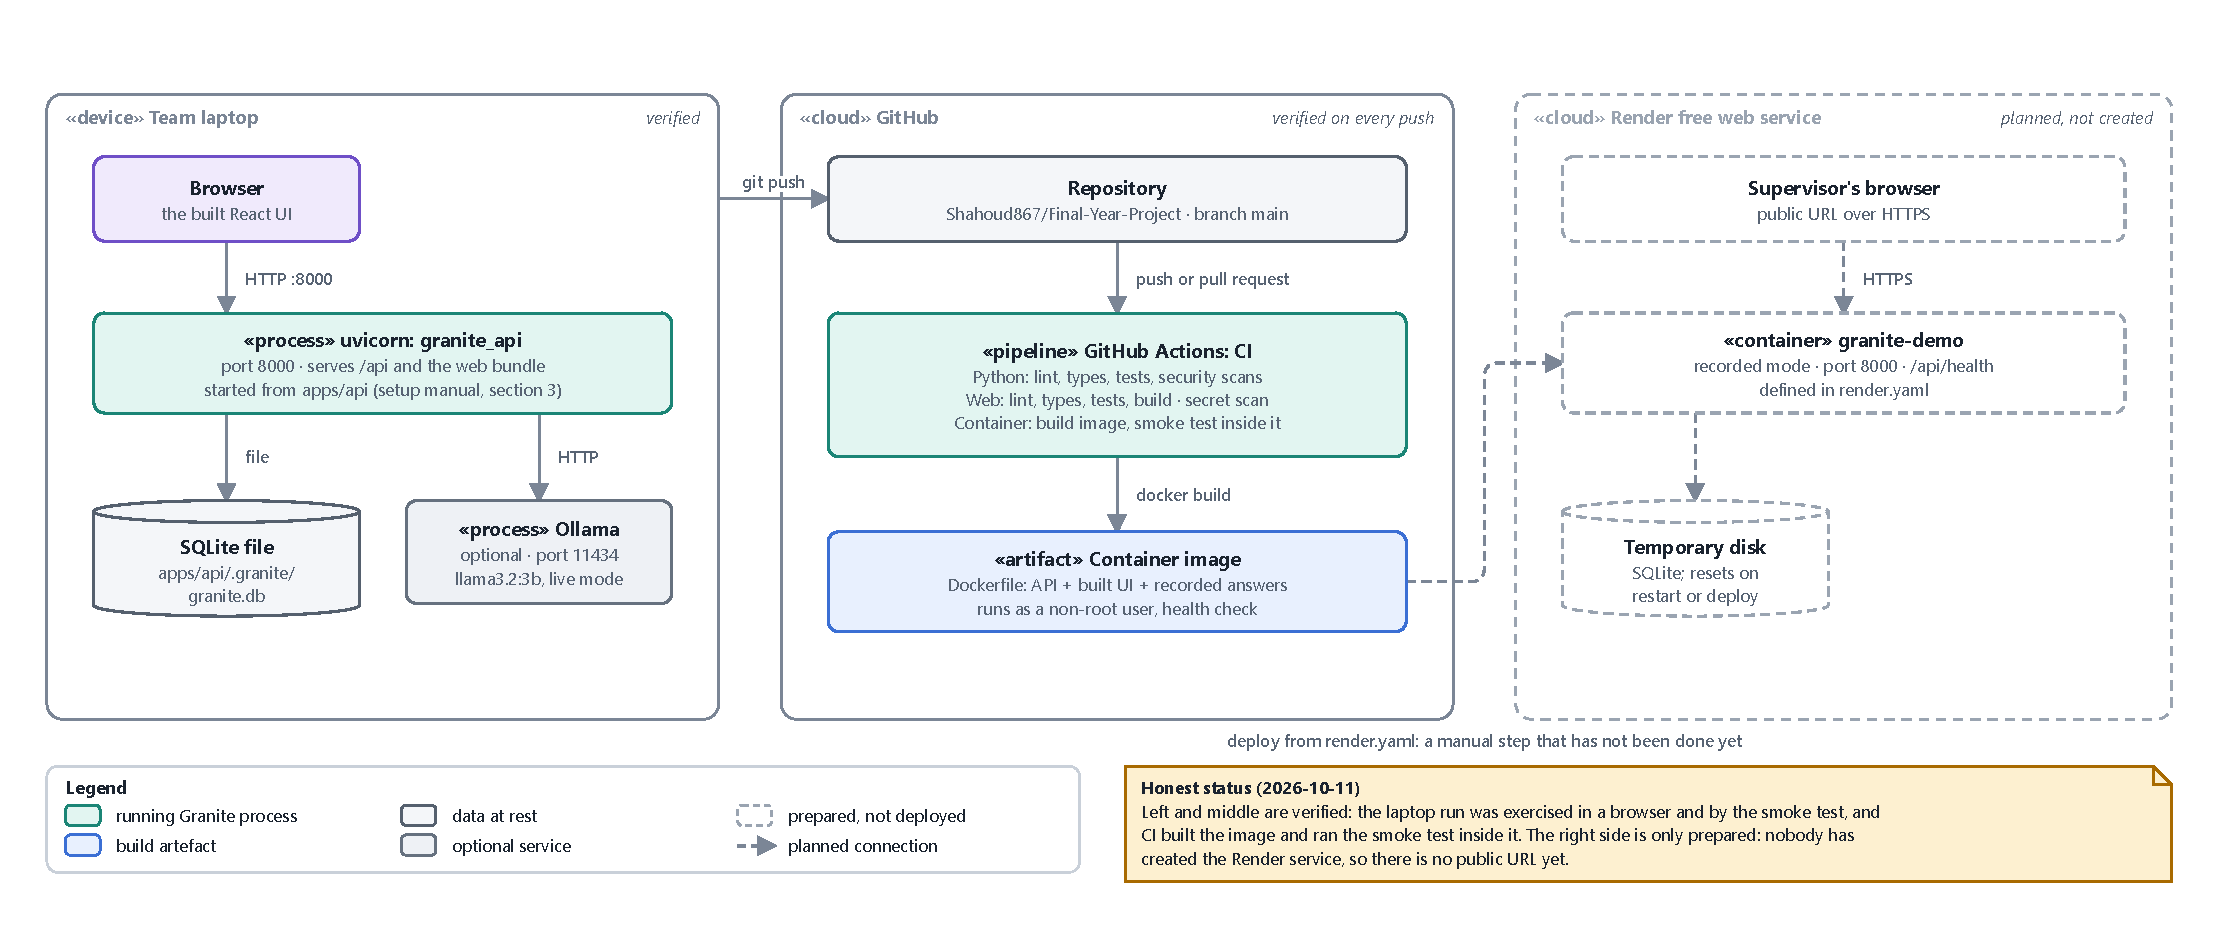
\includegraphics[width=\linewidth,height=0.42\textheight,keepaspectratio]{deployment-diagram.pdf}
\caption{Deployment diagram: verified and planned parts}
\label{fig:deployment}
\end{figure}


\begin{figure}[htbp]
\centering
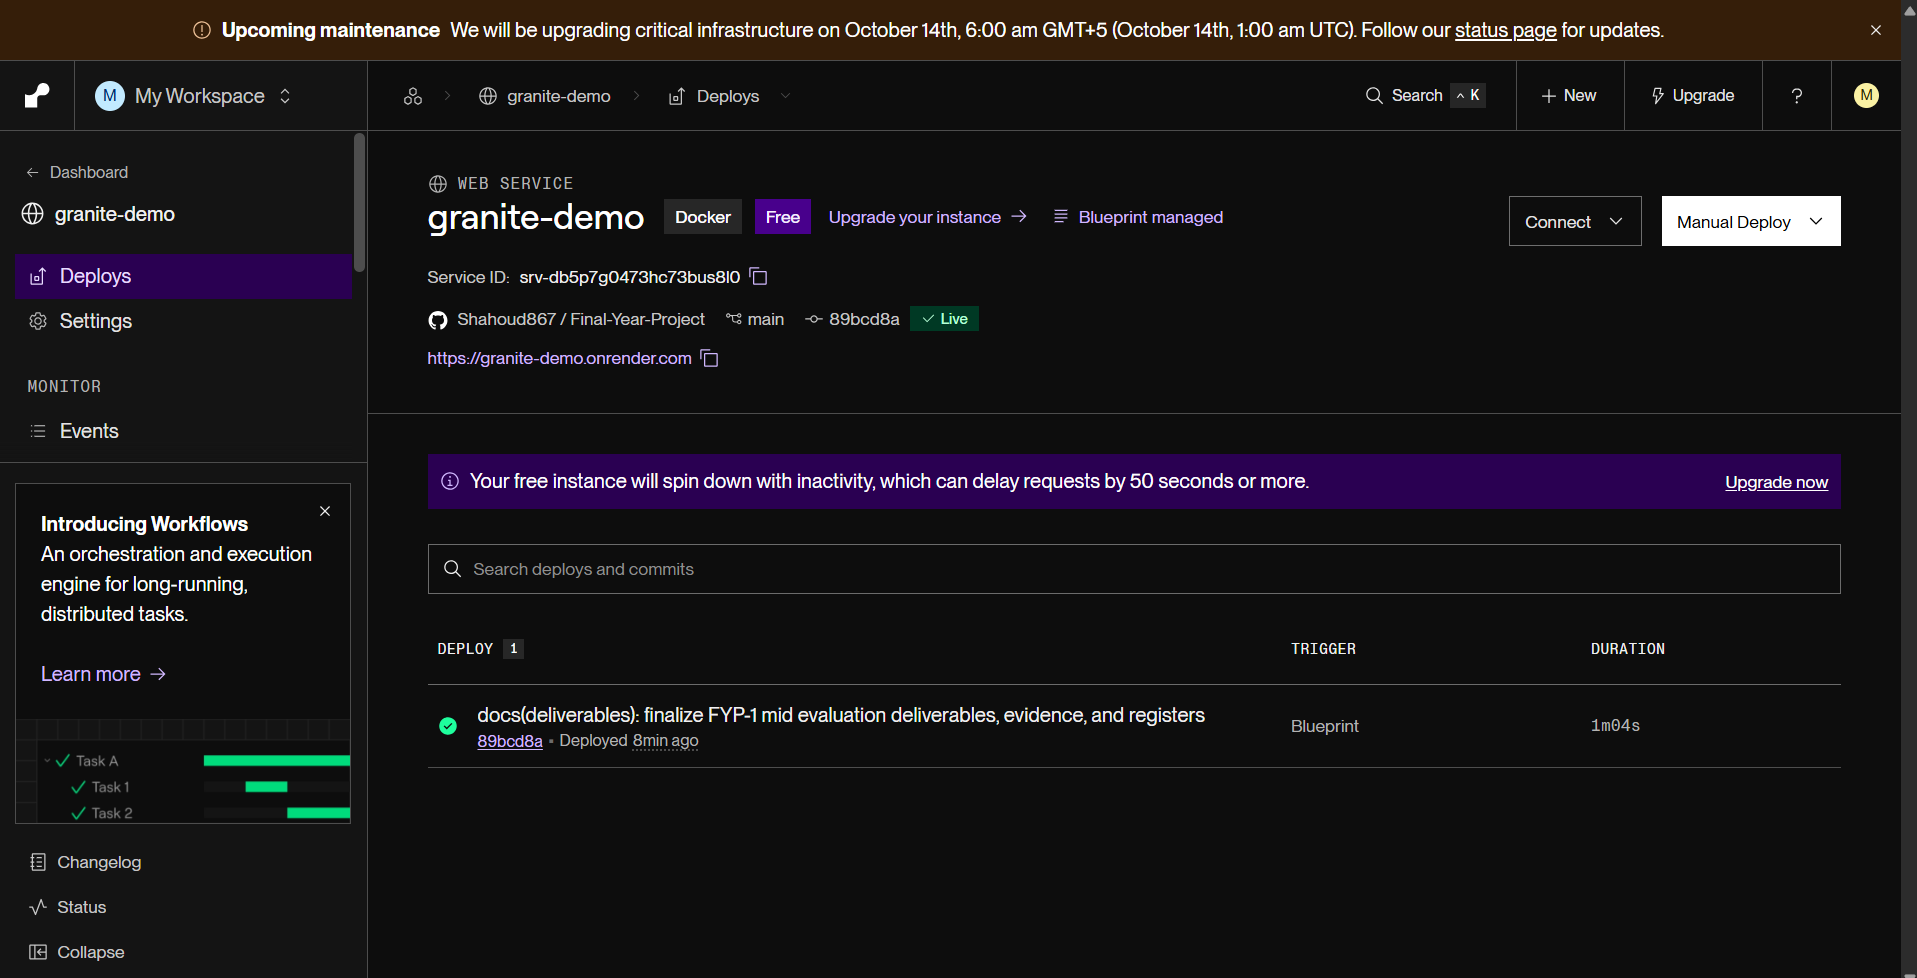
\includegraphics[width=\linewidth,height=0.42\textheight,keepaspectratio]{2026-10-11_render-service-live.png}
\caption{The granite-demo service live on Render}
\label{fig:render}
\end{figure}


\section{Tentative Timeline}

The timeline assumes that Week 1 of the semester began on 24 August.

{\small
\begin{longtable}{>{\raggedright\arraybackslash\hspace{0pt}}p{0.527\linewidth}>{\raggedright\arraybackslash\hspace{0pt}}p{0.187\linewidth}>{\raggedright\arraybackslash\hspace{0pt}}p{0.177\linewidth}}
\caption{Tentative Timeline}\label{tab:chapter10_fyp2_plan-2}\\
\toprule
\textbf{Milestone} & \textbf{Week} & \textbf{Dates} \\
\midrule
\endfirsthead
\toprule
\textbf{Milestone} & \textbf{Week} & \textbf{Dates} \\
\midrule
\endhead
\bottomrule
\endlastfoot
FYP-1 Mid evaluation; tag v0.1.0-mid1 & FYP-1 Week 9 & 12--16 Oct 2026 \\
Import, faults, check editor, redaction, fix suggestion & Weeks 9--10 & 19--30 Oct \\
SDK and LangGraph adapter; recovered runs; poster draft & Week 11 & 2--6 Nov \\
Fault Lab, evaluation harness, PDF export & Week 12 & 9--13 Nov \\
Poster submission; benchmark v0; usability pilot & Week 13 & 16--20 Nov \\
Report v2.0; non-owner install; evaluation screen & Week 14 & 23--27 Nov \\
FYP-1 Final and poster evaluation; v0.2.0 & Week 15 & 30 Nov -- 4 Dec \\
CrewAI, authentication, benchmark v1, evaluation v1 & FYP-2 Weeks 1--7 & Spring 2027 \\
FYP-2 Mid / Pre-Job-Fair; v0.5.0 & FYP-2 Week 8 & Spring 2027 \\
User acceptance testing & FYP-2 Weeks 9--11 & Spring 2027 \\
Job Fair & FYP-2 Weeks 12--14 & Spring 2027 \\
FYP-2 Final; v1.0.0 & FYP-2 Week 15 & Spring 2027 \\
Final deliverables to the committee & FYP-2 Weeks 17--18 & Spring 2027 \\
\end{longtable}
}

The team also sets internal deadlines ahead of external ones. Code is frozen 24 hours before every evaluation, report drafts go to the supervisor at least five days before each deadline, and the poster is sent to the supervisor at least five days before Week 13.

\section{Expected Final Deliverables}

Each remaining milestone has a defined set of deliverables. At FYP-1 Final the team will deliver:

\begin{itemize}
\item release 0.2.0, deployed
\item report version 2.0, covering both iterations, implementation details, the user manual and the FYP-2 and evaluation plans
\item the poster
\item the first benchmark and an evaluation with measured baselines
\item results of the usability pilot
\item records of four to six stakeholder interviews
\item a deployment record that includes an install by a non-owner
\end{itemize}

At FYP-2 Mid the deliverables are:

\begin{itemize}
\item release 0.5.0
\item a benchmark of at least 300 runs with a datasheet
\item an evaluation report with confidence intervals and ablations
\item a system test report and a defect list by severity
\item a security scan report
\item the acceptance-testing plan
\item an updated poster and report
\end{itemize}

For the Job Fair the team will prepare a booth demo with an offline fallback, a one-page handout with a QR code linking to the demo and repository, and the graduate directory materials.

The project closes at FYP-2 Final with release 1.0.0 and a final report signed by the supervisor. That report covers traceability, evaluation, limitations and individual contributions, and is accompanied by the acceptance-testing report, a handover package (source code, build and run instructions, dependencies, licences, known limitations and future work) and package and deployment diagrams. In Weeks 17 and 18 the final submission to the committee will include the report, the full presentation, references, the complete code, an executable with its README and user manual, and a passed plagiarism check. Throughout the project, the working deployed system, its source on GitHub, its manuals, design pack and registers remain the core product deliverables.

%======================================================================================
% conclusion
%======================================================================================
\chapter{Conclusion}

This report described the first iteration of Granite, a self-hostable workbench for investigating silent failures in multi-agent LLM workflows. Starting from a research gap that the failure-attribution literature names itself, silent failures that leave no anomaly signal, and from the panel's feedback that our proposal described mechanisms rather than a product, we redefined the project around one workflow and one unit of value, the verified finding. In the first iteration we built and deployed a working slice: a five-agent refund workflow on public retail data, executable checks against a source of truth, deterministic provenance attribution, verification by controlled replay with controls under a fixed verdict rule, human review and tamper-evident evidence. The system is covered by 381 automated tests and continuous integration, its design artefacts are generated from the code, and a pre-registered feasibility run met every threshold while catching a genuine model error and exposing one design limit.

The results are deliberately modest in scope: one workflow, one fault type, one small model and ten tasks, with no baseline comparison or user study yet. Process gaps remain as well, chiefly visible per-member ownership of the code, which we are addressing through reviewed pull requests and code walkthroughs. Iteration 2 broadens the inputs, workflows and fault types, adds repair and recovery, and produces the first evaluation against baselines, so that by FYP-1 Final the claims in this report can be tested on a labelled benchmark with clean controls.


\appendix
%======================================================================================
% appendix_action_register
%======================================================================================
\chapter{Proposal Action Register}

\begin{landscape}
{\footnotesize\setlength{\tabcolsep}{3pt}
\begin{longtable}{>{\raggedright\arraybackslash\hspace{0pt}}p{0.018\linewidth}>{\raggedright\arraybackslash\hspace{0pt}}p{0.043\linewidth}>{\raggedright\arraybackslash\hspace{0pt}}p{0.141\linewidth}>{\raggedright\arraybackslash\hspace{0pt}}p{0.048\linewidth}>{\raggedright\arraybackslash\hspace{0pt}}p{0.028\linewidth}>{\raggedright\arraybackslash\hspace{0pt}}p{0.028\linewidth}>{\raggedright\arraybackslash\hspace{0pt}}p{0.199\linewidth}>{\raggedright\arraybackslash\hspace{0pt}}p{0.173\linewidth}>{\raggedright\arraybackslash\hspace{0pt}}p{0.147\linewidth}}
\caption{Proposal Action Register}\label{tab:appendix_action_register-1}\\
\toprule
\textbf{ID} & \textbf{Source} & \textbf{Panel comment} & \textbf{Owner} & \textbf{Due} & \textbf{Status} & \textbf{Action taken} & \textbf{Evidence} & \textbf{Remaining step} \\
\midrule
\endfirsthead
\toprule
\textbf{ID} & \textbf{Source} & \textbf{Panel comment} & \textbf{Owner} & \textbf{Due} & \textbf{Status} & \textbf{Action taken} & \textbf{Evidence} & \textbf{Remaining step} \\
\midrule
\endhead
\bottomrule
\endlastfoot
A1 & Defense, 11 Sep 2026 & "UI/UX needs improvement." & Shahoud (design system); all for their screens & Mid-1 & Partly & Five task-oriented screens; one vocabulary; four-stage stepper; loading, empty and error states; light/dark; keyboard-operable graph; phone layout; plain field messages; automated accessibility checks; before/after comparison with the defense PoC; usability protocol with thresholds & \texttt{evidence/\allowbreak{}demos/\allowbreak{}} screenshots; \texttt{2026-10-13\_\allowbreak{}ui-before-after.\allowbreak{}md}; accessibility audit; usability protocol & Run the usability check with three outside participants \\
A2 & Defense & "Features are not sufficiently clear." & All & Mid-1 & Done & Eight features in one fixed order with purpose, inputs and outputs; same list as an in-app page & Feature catalogue; guide page & Report section (this report) \\
A3 & Defense & "Unclear what inputs each feature will accept." & All & Mid-1 & Done & Every input typed, limited and refused with a message; trace JSON Schema; API docs; test keeps the guide equal to server limits & Data dictionary; validation tests & Inputs of features not yet built \\
A4 & Defense & "Unclear how flaws will be verified and results captured." & Saif & Mid-1 & Done & Levels V0--V3; N replays + M controls; VR-1; Wilson interval; hashed evidence; review records; report & Verification sequence; decision-table tests; feasibility results & Larger evaluation \\
A5 & Defense & "Overall workflow must be redefined." & All & Mid-1 & Done & One workflow enforced by a state machine and shown as a stepper; flow and activity diagrams & State machine; activity diagram & Supervisor signature on change record C-01 \\
A6 & Implicit & PoC showed research, not a product & Saif; all & Mid-1 & Partly & Working slice; CI on GitHub; public deployment on Render (11 Oct); CD workflow & Live URL; CI/CD runs; deployment record (PR \#1) & Deploy-hook secret, branch protection, tag v0.1.0-mid1, PRs from every member \\
\end{longtable}
}
\end{landscape}

%======================================================================================
% appendix_requirements
%======================================================================================
\chapter{Detailed Requirements}

{\small
\begin{longtable}{>{\raggedright\arraybackslash\hspace{0pt}}p{0.122\linewidth}>{\raggedright\arraybackslash\hspace{0pt}}p{0.577\linewidth}>{\raggedright\arraybackslash\hspace{0pt}}p{0.044\linewidth}>{\raggedright\arraybackslash\hspace{0pt}}p{0.117\linewidth}}
\caption{Detailed Requirements}\label{tab:appendix_requirements-1}\\
\toprule
\textbf{ID} & \textbf{Requirement} & \textbf{Pri.} & \textbf{Milestone} \\
\midrule
\endfirsthead
\toprule
\textbf{ID} & \textbf{Requirement} & \textbf{Pri.} & \textbf{Milestone} \\
\midrule
\endhead
\bottomrule
\endlastfoot
FR-IMP-01 & Import Granite Trace v1 and Who\&When JSON ($\leq$ 5 MB, $\leq$ 500 steps) with a validation report giving the JSON path of every error & M & Final-1 \\
FR-IMP-02 & Imported runs are marked non-replayable and get evidence-level verification only & M & Final-1 \\
FR-SDK-01 & Python SDK captures a LangGraph workflow's node inputs and outputs into Granite Trace v1 via a decorator or callback & M & Final-1 \\
FR-SDK-02 & CrewAI adapter & M & Mid-2 \\
FR-CHK-05 & Create, edit (versioned), dry-run and disable checks from the UI & M & Final-1 \\
FR-ATT-03 & Tracing terminates on cyclic lineage within a revisit bound (default 3) & M & Final-1 \\
FR-ATT-04 & Optional LLM second-opinion hypothesis, labelled unverified & S & Final-1 (M at Mid-2) \\
FR-VER-04 & Verification refused with a message for non-replayable runs & M & Final-1 \\
FR-VER-05 & Partial experiments keep completed replays, verdict ERROR, and can resume & M & Final-1 \\
FR-FIX-01 & Suggest a fix (one atomic field value or one prompt patch) and verify it as a fix experiment & M & Final-1 \\
FR-FIX-02 & Promote a passing replay of a confirmed fix to a recovered run & M & Final-1 \\
FR-FIX-03 & Store verified fixes by signature and suggest them for new findings & S & Mid-2 \\
FR-REP-02 & Export a regression case (JSON + pytest) runnable in recorded mode in CI & M & Final-1 \\
FR-LAB-01 & Batch-generate labelled runs over workflow $\times$ runtime $\times$ fault with a clean-control share (default 20\%) & M & Final-1 \\
FR-EVA-01 & Compute detection recall, false-alarm rate, top-1/top-3 origin accuracy, verdict precision and recovery rate with bootstrap 95\% intervals, against last-agent and LLM-judge baselines & M & Final-1 v0 / Mid-2 v1 \\
FR-AUTH-01 & Sign in with GitHub; reviews record the authenticated identity & S & Mid-2 \\
FR-ADM-01 & Delete a run and its derived records; configure retention & S & Mid-2 \\
\end{longtable}
}

Non-functional requirements NFR-01 to NFR-15 are listed in Section 4.5.

%======================================================================================
% appendix_test_cases
%======================================================================================
\chapter{Detailed Test Cases}

{\small
\begin{longtable}{>{\raggedright\arraybackslash\hspace{0pt}}p{0.146\linewidth}>{\raggedright\arraybackslash\hspace{0pt}}p{0.452\linewidth}>{\raggedright\arraybackslash\hspace{0pt}}p{0.165\linewidth}>{\raggedright\arraybackslash\hspace{0pt}}p{0.098\linewidth}}
\caption{Detailed Test Cases}\label{tab:appendix_test_cases-1}\\
\toprule
\textbf{ID} & \textbf{Test case} & \textbf{Requirement area} & \textbf{Result} \\
\midrule
\endfirsthead
\toprule
\textbf{ID} & \textbf{Test case} & \textbf{Requirement area} & \textbf{Result} \\
\midrule
\endhead
\bottomrule
\endlastfoot
SYS-CORE-01 & Full investigation of a silent failure & Run, detect, trace back, verify, review, report & Pass \\
SYS-CORE-02 & A clean run raises no alarm & Detect & Pass \\
SYS-CORE-03 & Refute a wrong hypothesis, then confirm the right one & Verify & Pass \\
SYS-CORE-04 & The run graph marks the failing steps & Inspect & Pass \\
SYS-CORE-05 & Runs and findings can be found again & History & Pass \\
SYS-CORE-06 & The interface is documented by the running system & Guide / API docs & Pass \\
SYS-CORE-07 & The web interface is delivered by the same server & Deployment & Pass \\
SYS-ERR-01 & Invalid input is refused with one message per field & Input validation & Pass \\
SYS-ERR-02 & Asking for something that does not exist & Errors & Pass \\
SYS-ERR-03 & The lifecycle cannot be skipped & Review, lifecycle & Pass (intermittent failure fixed as D-26) \\
SYS-ERR-04 & Recorded mode cannot answer a task nobody recorded & Run & Pass \\
SYS-ERR-05 & A hypothesis that cannot be tested is refused, not guessed & Verify & Pass \\
SYS-ERR-06 & Limits are enforced & Security & Pass \\
SYS-ERR-07 & The language model is down & Reliability & Pass \\
SYS-SEC-01 & Every response carries the security headers & Security & Pass \\
SYS-SEC-02 & Evidence is append-only & Evidence & Pass \\
SYS-SEC-03 & Ground truth stays out of the evidence & Attribution integrity & Pass \\
SYS-SEC-04 & With a token configured, nothing but health is public & Security & Pass \\
SYS-SEC-05 & Too many state-changing requests are throttled & Security & Pass \\
SYS-REL-01 & A restart loses nothing & Reliability & Pass \\
SYS-REL-02 & Concurrent work is not lost & Reliability & Pass \\
SYS-REL-03 & Recorded runs are reproducible & Determinism & Pass \\
\end{longtable}
}

%======================================================================================
% appendix_repository
%======================================================================================
\chapter{Repository and Contribution Evidence}

Repository: \url{https://github.com/Shahoud867/Final-Year-Project} (private; the supervisor needs read access). Branching method: \texttt{.\allowbreak{}github/\allowbreak{}CONTRIBUTING.\allowbreak{}md} and ADR-010. CI record: run 37924480165 (9 Oct) and run 38137714669 (11 Oct); CD run 38137856992 (11 Oct). Deployment: \texttt{evidence/\allowbreak{}repo/\allowbreak{}2026-10-11\_\allowbreak{}render-deployment.\allowbreak{}md}.

\textbf{Note on the template:} the prescribed LaTeX template was used unchanged in style. Four rendering defects were corrected so the template compiles as intended: the contents, figure and table lists were printed twice by the class file; the project title and student names used on the Students' Submission page were not defined; the \texttt{longtable} package used by the template's tables was not loaded; and the front-matter lists and the submission table were run together on one page.

%======================================================================================
% appendix_diagrams
%======================================================================================
\chapter{Additional Design Diagrams}

{\small
\begin{longtable}{>{\raggedright\arraybackslash\hspace{0pt}}p{0.104\linewidth}>{\raggedright\arraybackslash\hspace{0pt}}p{0.411\linewidth}>{\raggedright\arraybackslash\hspace{0pt}}p{0.375\linewidth}}
\caption{Additional Design Diagrams}\label{tab:appendix_diagrams-1}\\
\toprule
\textbf{Figure} & \textbf{Diagram} & \textbf{File} \\
\midrule
\endfirsthead
\toprule
\textbf{Figure} & \textbf{Diagram} & \textbf{File} \\
\midrule
\endhead
\bottomrule
\endlastfoot
E.1 & Domain model / class diagram & \texttt{domain-model.\allowbreak{}svg} \\
E.2 & Component diagram & \texttt{component-diagram.\allowbreak{}svg} \\
E.3 & Layer diagram & \texttt{layer-diagram.\allowbreak{}svg} \\
E.4 & Structure chart & \texttt{structure-chart.\allowbreak{}svg} \\
E.5 & Investigation flow diagram & \texttt{investigation-flow.\allowbreak{}svg} \\
E.6 & DFD level 0 (context) & \texttt{dfd-context.\allowbreak{}svg} \\
E.7 & DFD level 1 & \texttt{dfd-level-1.\allowbreak{}svg} \\
E.8 & Activity diagram (five swimlanes) & \texttt{activity-investigation.\allowbreak{}svg} \\
E.9 & Finding state machine & \texttt{finding-state-machine.\allowbreak{}svg} \\
E.10 & Refund Desk data-flow graph & \texttt{refund-desk-dataflow.\allowbreak{}svg} \\
E.11 & Call graph (38 functions, 49 calls) & \texttt{call-graph.\allowbreak{}svg} \\
E.12 & Run sequence diagram & \texttt{run-sequence.\allowbreak{}svg} \\
E.13 & Verification sequence diagram & \texttt{verification-sequence.\allowbreak{}svg} \\
E.14 & Interaction overview diagram & \texttt{interaction-overview.\allowbreak{}svg} \\
E.15 & ER diagram & \texttt{database-schema.\allowbreak{}svg} \\
E.16 & Deployment diagram & \texttt{deployment-diagram.\allowbreak{}svg} \\
E.17 & Use case diagram & \texttt{use-case-diagram.\allowbreak{}svg} \\
E.18 & Algorithm diagrams (check language, attribution, VR-1, replay plan) & \texttt{algorithm-design.\allowbreak{}md} \\
\end{longtable}
}

\begin{figure}[htbp]
\centering
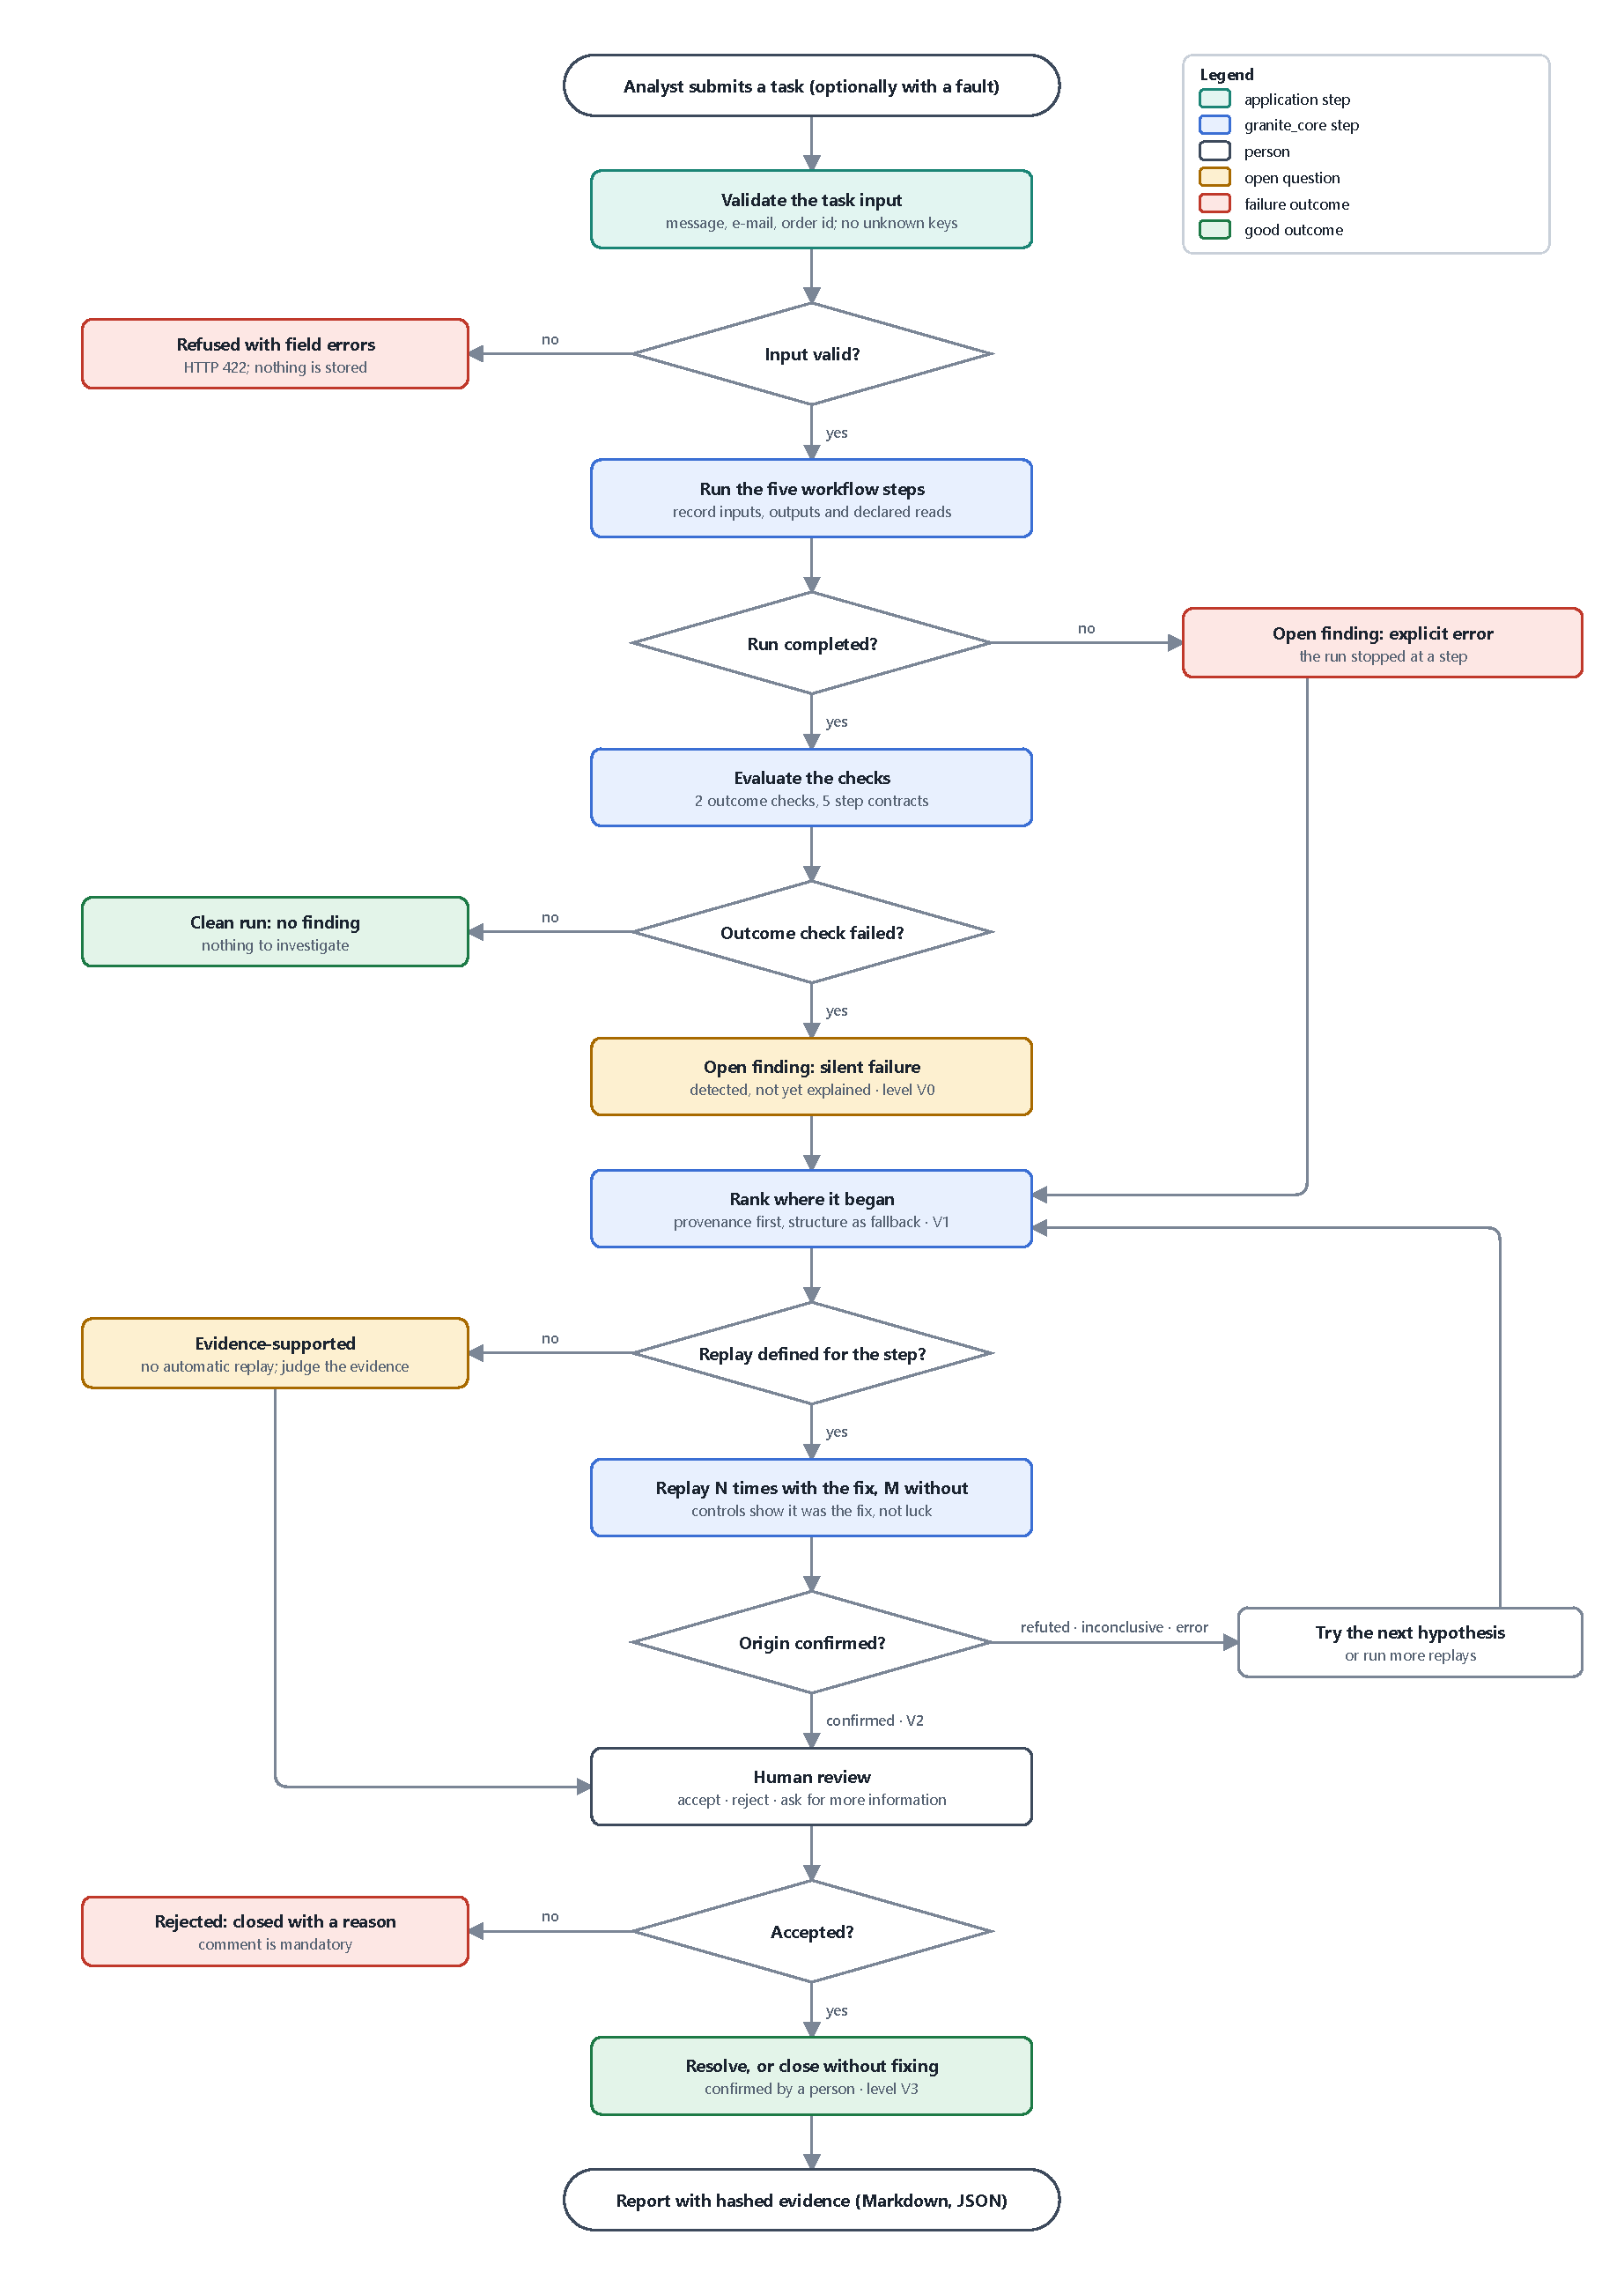
\includegraphics[width=\linewidth,height=0.62\textheight,keepaspectratio]{investigation-flow.pdf}
\caption{Investigation flow diagram}
\label{fig:app-flow}
\end{figure}


\begin{figure}[htbp]
\centering
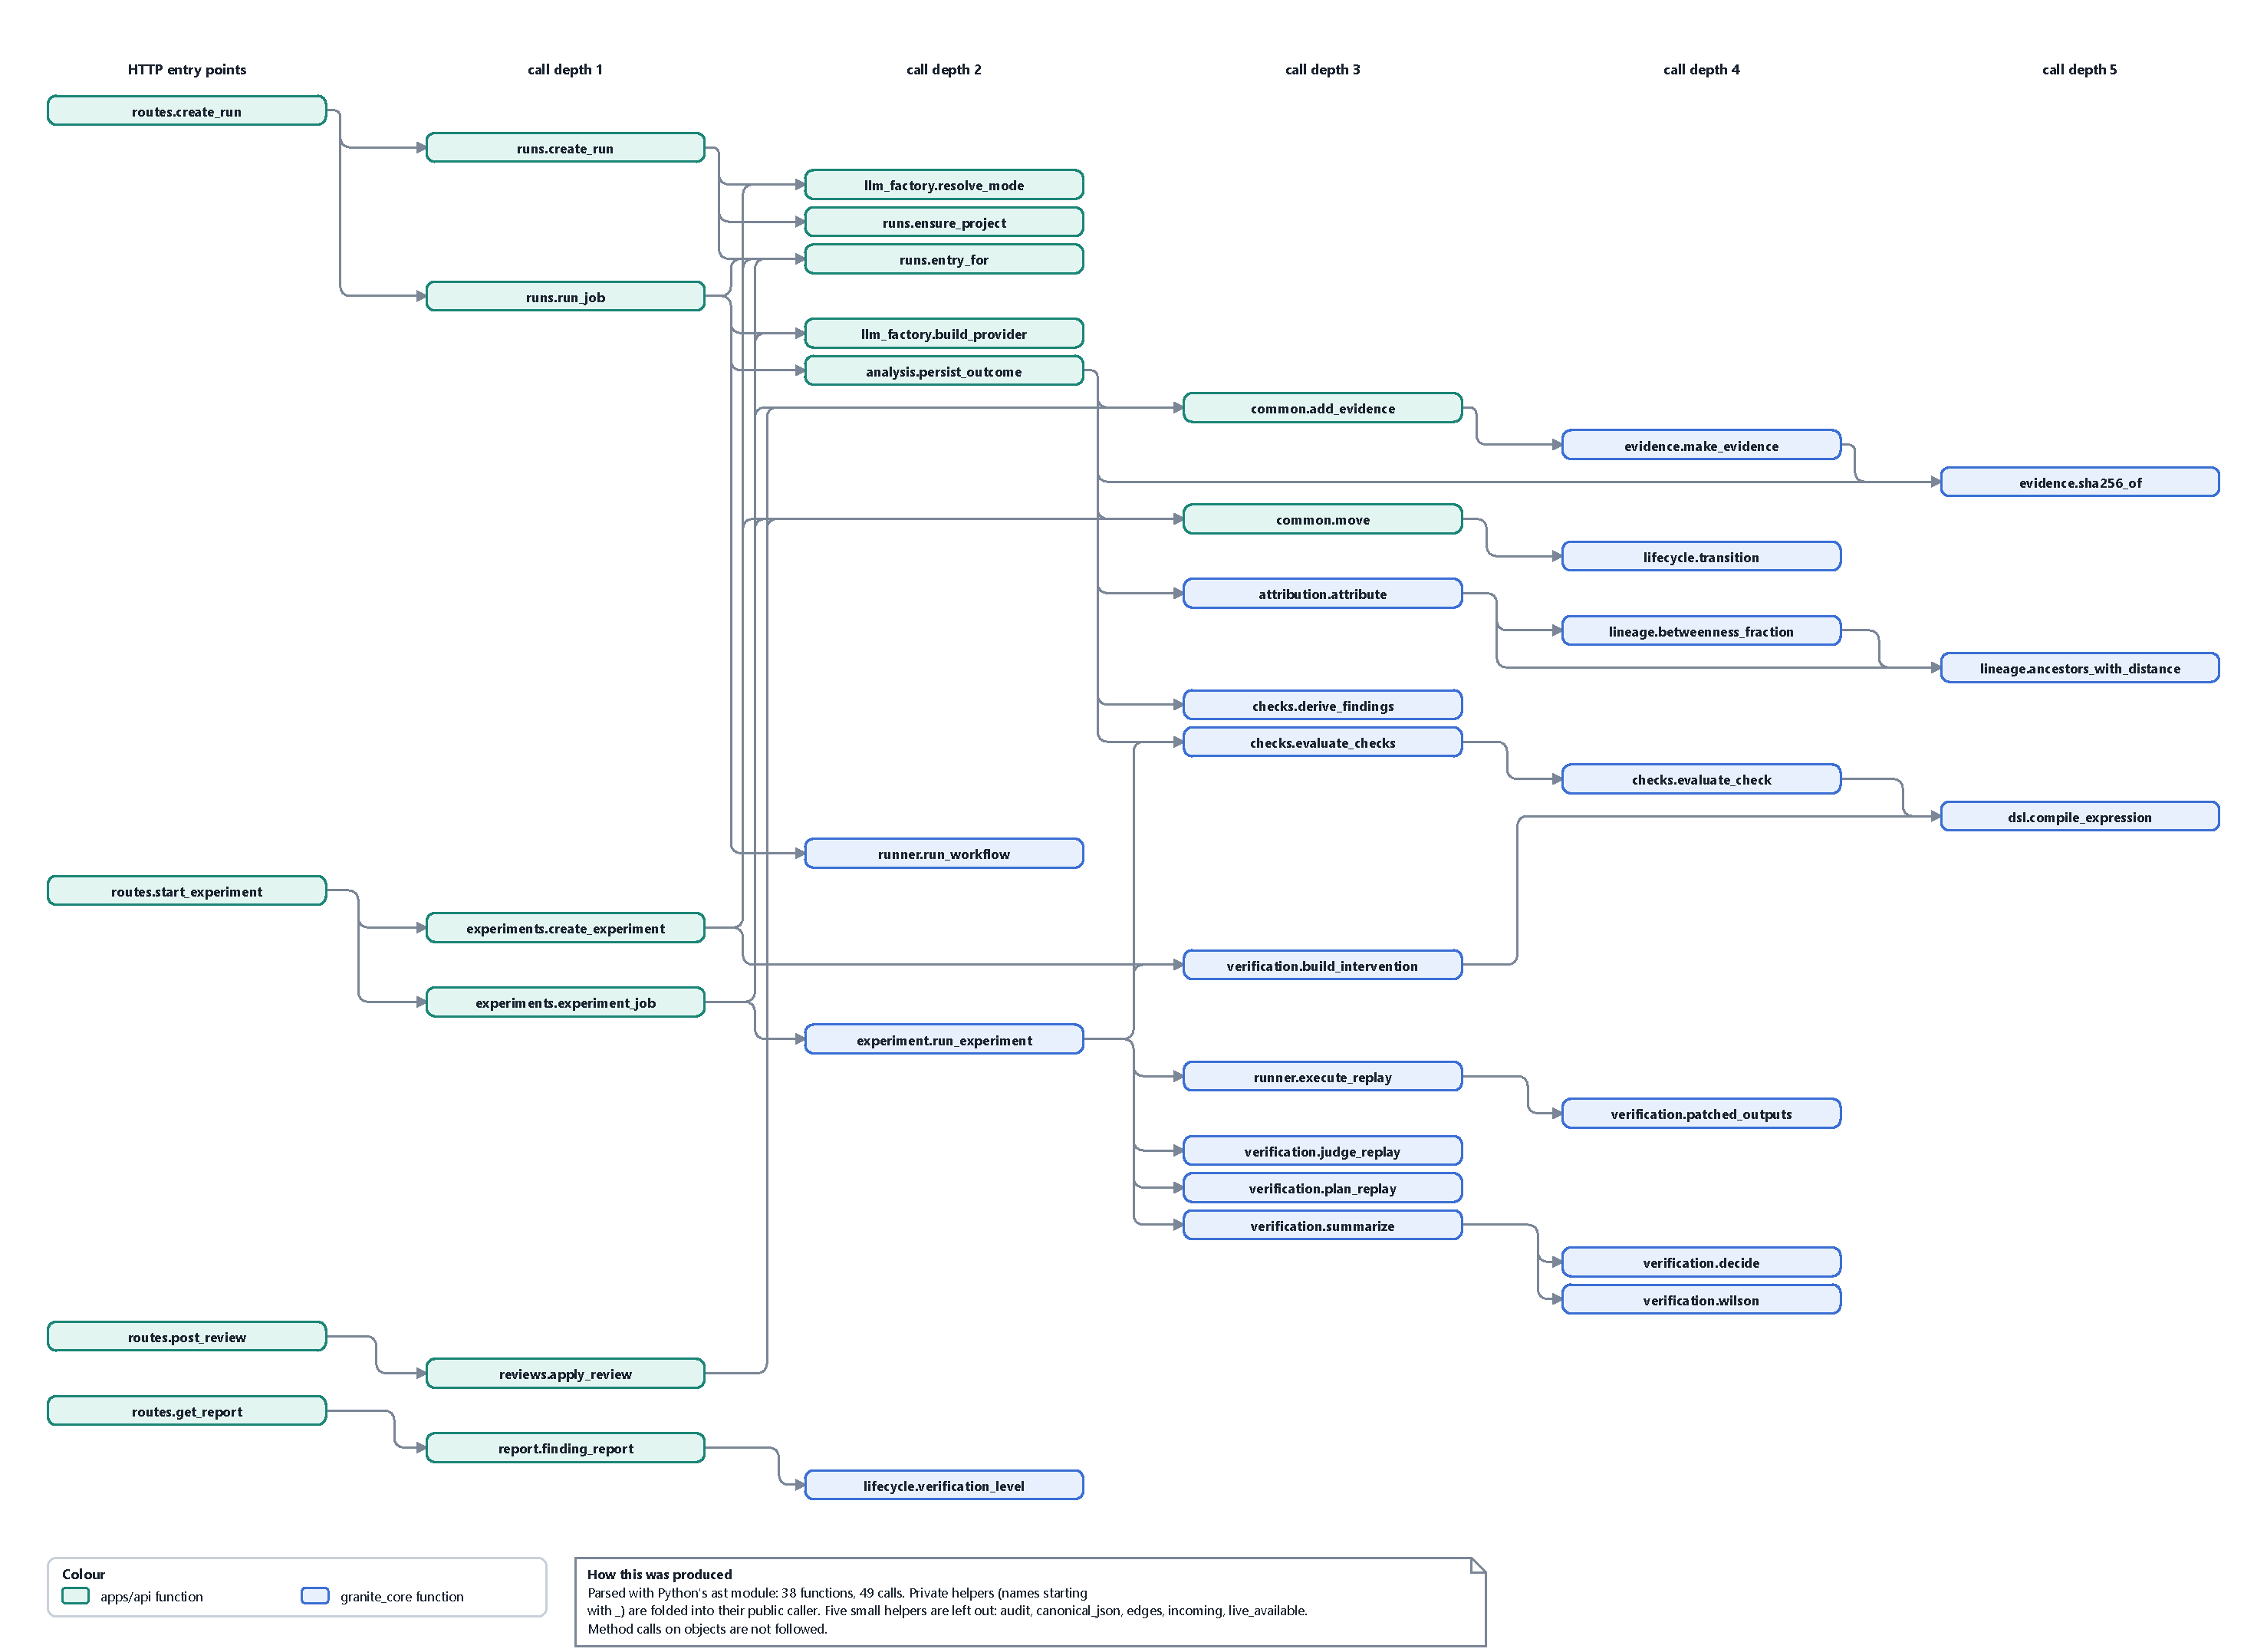
\includegraphics[width=\linewidth,height=0.42\textheight,keepaspectratio]{call-graph.pdf}
\caption{Call graph computed from the source (38 functions, 49 calls)}
\label{fig:app-callgraph}
\end{figure}


\begin{figure}[htbp]
\centering
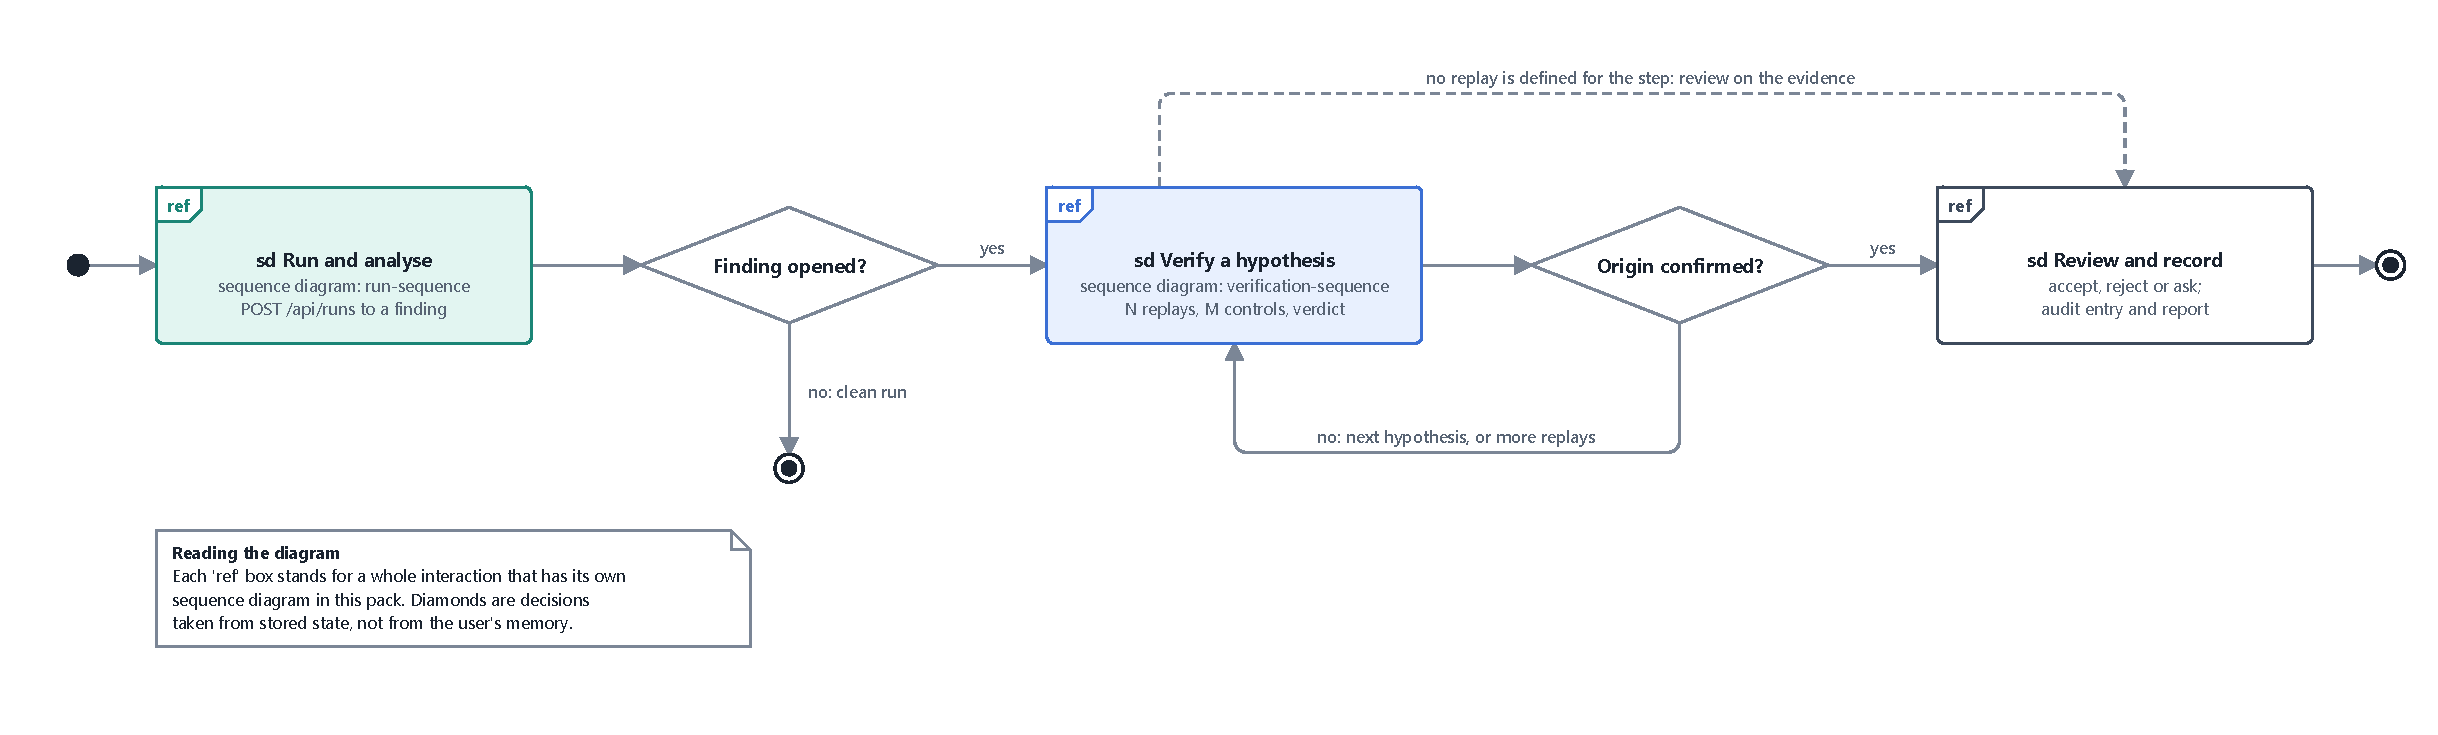
\includegraphics[width=\linewidth,height=0.42\textheight,keepaspectratio]{interaction-overview.pdf}
\caption{Interaction overview diagram}
\label{fig:app-interaction}
\end{figure}

%======================================================================================
% appendix_meetings
%======================================================================================
\chapter{Meeting and Progress Evidence}

{\small
\begin{longtable}{>{\raggedright\arraybackslash\hspace{0pt}}p{0.080\linewidth}>{\raggedright\arraybackslash\hspace{0pt}}p{0.144\linewidth}>{\raggedright\arraybackslash\hspace{0pt}}p{0.296\linewidth}>{\raggedright\arraybackslash\hspace{0pt}}p{0.341\linewidth}}
\caption{Meeting and Progress Evidence}\label{tab:appendix_meetings-1}\\
\toprule
\textbf{Date} & \textbf{Attendees} & \textbf{Discussed / decided} & \textbf{Actions (owner, due)} \\
\midrule
\endfirsthead
\toprule
\textbf{Date} & \textbf{Attendees} & \textbf{Discussed / decided} & \textbf{Actions (owner, due)} \\
\midrule
\endhead
\bottomrule
\endlastfoot
11 Sep 2026 & Panel, supervisor, team & Proposal defense: approved with five comments (A1--A5) & Redefine workflow; improve UI/UX; define inputs and verification \\
\end{longtable}
}

The table above lists the meetings recorded in the project repository. Progress since the defense is recorded in the milestone log and the repository history; the main dated milestones are listed below.

{\small
\begin{longtable}{>{\raggedright\arraybackslash\hspace{0pt}}p{0.113\linewidth}>{\raggedright\arraybackslash\hspace{0pt}}p{0.504\linewidth}>{\raggedright\arraybackslash\hspace{0pt}}p{0.273\linewidth}}
\caption{Meeting and Progress Evidence}\label{tab:appendix_meetings-2}\\
\toprule
\textbf{Date} & \textbf{Milestone} & \textbf{Evidence} \\
\midrule
\endfirsthead
\toprule
\textbf{Date} & \textbf{Milestone} & \textbf{Evidence} \\
\midrule
\endhead
\bottomrule
\endlastfoot
6 Oct 2026 & Master plan revised (v1.1); workflow redefined around the verified finding; repository reorganised; core library and Refund Desk working & Master plan; change record C-01; commits on \texttt{main} \\
7 Oct 2026 & API, web interface, CI definition; pre-registered feasibility run (all six thresholds met) & Feasibility results; demo screenshots \\
9 Oct 2026 & Code on GitHub; first green CI run including container build and smoke test & CI run 37924480165 \\
11 Oct 2026 & Design pack (21 diagrams), system tests, CD workflow, registers; public deployment on Render; first pull requests & CI/CD runs; deployment record; PR \#1, PR \#2 \\
13 Oct 2026 & Before/after UI comparison and usability-check protocol for panel action A1 & PR \#3 \\
\end{longtable}
}

\textbf{Progress evidence:} the milestone log (\texttt{docs/\allowbreak{}registers/\allowbreak{}milestone-log.\allowbreak{}md}) with planned and actual dates, the delays and recovery plan in Section 3.8, and the change log entries C-01 to C-03.


\bibliographystyle{IEEEtran}
\bibliography{references/references}
\end{document}
